% Arquivo LaTeX de exemplo de dissertação/tese a ser apresentada à CPG do IME-USP
%
% Criação: Jesús P. Mena-Chalco
% Revisão: Fabio Kon e Paulo Feofiloff
% Adaptação para UTF8, biblatex e outras melhorias: Nelson Lago
%
% Except where otherwise indicated, these files are distributed under
% the MIT Licence. The example text, which includes the tutorial and
% examples as well as the explanatory comments in the source, are
% available under the Creative Commons Attribution International
% Licence, v4.0 (CC-BY 4.0) - https://creativecommons.org/licenses/by/4.0/


%%%%%%%%%%%%%%%%%%%%%%%%%%%%%%%%%%%%%%%%%%%%%%%%%%%%%%%%%%%%%%%%%%%%%%%%%%%%%%%%
%%%%%%%%%%%%%%%%%%%%%%%%%%%%%%% PREÂMBULO LaTeX %%%%%%%%%%%%%%%%%%%%%%%%%%%%%%%%
%%%%%%%%%%%%%%%%%%%%%%%%%%%%%%%%%%%%%%%%%%%%%%%%%%%%%%%%%%%%%%%%%%%%%%%%%%%%%%%%

% A opção twoside (frente-e-verso) significa que a aparência das páginas pares
% e ímpares pode ser diferente. Por exemplo, as margens podem ser diferentes ou
% os números de página podem aparecer à direita ou à esquerda alternadamente.
% Mas nada impede que você crie um documento "só frente" e, ao imprimir, faça
% a impressão frente-e-verso.
%
% Aqui também definimos a língua padrão do documento (a última da lista) e
% línguas adicionais. Para teses do IME, no mínimo português e inglês são
% obrigatórios, porque independentemente da língua principal do texto é
% preciso fornecer o resumo nessas duas línguas. LaTeX aceita alguns nomes
% diferentes para a língua portuguesa; dentre as opções, prefira sempre
% "brazilian" para português brasileiro e "portuguese" para português europeu.
%\documentclass[a4paper,12pt,twoside,brazilian,english]{book}
\documentclass[a4paper,12pt,twoside,english,brazilian]{book}

% Vários pacotes e opções de configuração genéricos; para personalizar o
% resultado, modifique estes arquivos.
\usepackage{imegoodies}
\usepackage[thesis]{imelooks}

%\nocolorlinks % para impressão em P&B

% Diretórios onde estão as figuras; com isso, não é preciso colocar o caminho
% completo em \includegraphics (e nem a extensão).
\graphicspath{{figuras/},{logos/}}

% Comandos rápidos para mudar de língua:
% \en -> muda para o inglês
% \br -> muda para o português
% \texten{blah} -> o texto "blah" é em inglês
% \textbr{blah} -> o texto "blah" é em português
\babeltags{br = brazilian, en = english}

\input{extras/source-code}

%%%%%%%%%%%%%%%%%%%%%%%%%%%%%%%%%%%%%%%%%%%%%%%%%%%%%%%%%%%%%%%%%%%%%%%%%%%%%%%%
%%%%%%%%%%%%%%%%%%%%%%%%%%%%%%%%%% METADADOS %%%%%%%%%%%%%%%%%%%%%%%%%%%%%%%%%%%
%%%%%%%%%%%%%%%%%%%%%%%%%%%%%%%%%%%%%%%%%%%%%%%%%%%%%%%%%%%%%%%%%%%%%%%%%%%%%%%%

% O arquivo com os dados bibliográficos para biblatex; você pode usar
% este comando mais de uma vez para acrescentar múltiplos arquivos
\addbibresource{bibliografia.bib}

% Este comando permite acrescentar itens à lista de referências sem incluir
% uma referência de fato no texto (pode ser usado em qualquer lugar do texto)
%\nocite{bronevetsky02,schmidt03:MSc, FSF:GNU-GPL, CORBA:spec, MenaChalco08}
% Com este comando, todos os itens do arquivo .bib são incluídos na lista
% de referências
%\nocite{*}

% É possível definir como determinadas palavras podem (ou não) ser
% hifenizadas; no entanto, a hifenização automática geralmente funciona bem
\babelhyphenation{documentclass latexmk soft-ware clsguide} % todas as línguas
\babelhyphenation[brazilian]{Fu-la-no}
\babelhyphenation[english]{what-ever}

% Estes comandos definem o título e autoria do trabalho e devem sempre ser
% definidos, pois além de serem utilizados para criar a capa, também são
% armazenados nos metadados do PDF.
\title{
    % Obrigatório nas duas línguas
    titlept={Título do trabalho},
    titleen={Title of the document},
    % Opcional, mas se houver deve existir nas duas línguas
    subtitlept={um subtítulo},
    subtitleen={a subtitle},
}

\author[fem]{Nome Completo}

% Para TCCs, este comando define o supervisor
\orientador[fem]{Profª. Drª. Fulana de Tal}

% Se não houver, remova; se houver mais de um, basta
% repetir o comando quantas vezes forem necessárias
\coorientador{Prof. Dr. Ciclano de Tal}
\coorientador[fem]{Profª. Drª. Beltrana de Tal}

% A página de rosto da versão para depósito (ou seja, a versão final
% antes da defesa) deve ser diferente da página de rosto da versão
% definitiva (ou seja, a versão final após a incorporação das sugestões
% da banca).
\defesa{
  nivel=mestrado, % mestrado, doutorado ou tcc
  % É a versão para defesa ou a versão definitiva?
  %definitiva,
  % É qualificação?
  %quali,
  programa={Ciência da Computação},
  membrobanca={Profª. Drª. Fulana de Tal (orientadora) -- IME-USP [sem ponto final]},
  % Em inglês, não há o "ª"
  %membrobanca{Prof. Dr. Fulana de Tal (advisor) -- IME-USP [sem ponto final]},
  membrobanca={Prof. Dr. Ciclano de Tal -- IME-USP [sem ponto final]},
  membrobanca={Profª. Drª. Convidada de Tal -- IMPA [sem ponto final]},
  % Se não houve bolsa, remova
  %
  % Norma sobre agradecimento por auxílios da FAPESP:
  % https://fapesp.br/11789/referencia-ao-apoio-da-fapesp-em-todas-as-formas-de-divulgacao
  %
  % Norma sobre agradecimento por auxílios da CAPES (Portaria 206,
  % de 4 de Setembro de 2018):
  % https://www.in.gov.br/materia/-/asset_publisher/Kujrw0TZC2Mb/content/id/39729251/do1-2018-09-05-portaria-n-206-de-4-de-setembro-de-2018-39729135
  %
  %apoio={O presente trabalho foi realizado com apoio da Coordenação
  %       de Aperfeiçoamento\\ de Pessoal de Nível Superior -- Brasil
  %       (CAPES) -- Código de Financiamento 001}, % o código é sempre 001
  %
  %apoio={This study was financed in part by the Coordenação de
  %       Aperfeiçoamento\\ de Pessoal de Nível Superior -- Brasil
  %       (CAPES) -- Finance Code 001}, % o código é sempre 001
  %
  %apoio={Durante o desenvolvimento deste trabalho, o autor recebeu\\
  %       auxílio financeiro da FAPESP -- processo nº aaaa/nnnnn-d},
  %
  %apoio={During the development if this work, the author received\\
  %       financial support from FAPESP -- grant \#aaaa/nnnnn-d},
  %
  apoio={Durante o desenvolvimento deste trabalho o autor
         recebeu auxílio financeiro da XXXX},
  local={São Paulo},
  data=2017-08-10, % YYYY-MM-DD
  % A licença do seu trabalho. Use CC-BY, CC-BY-NC, CC-BY-ND, CC-BY-SA,
  % CC-BY-NC-SA ou CC-BY-NC-ND para escolher a licença Creative Commons
  % correspondente (o sistema insere automaticamente o texto da licença).
  % Se quiser estabelecer regras diferentes para o uso de seu trabalho,
  % converse com seu orientador e coloque o texto da licença aqui, mas
  % observe que apenas TCCs sob alguma licença Creative Commons serão
  % acrescentados ao BDTA. Se você tem alguma intenção de publicar o
  % trabalho comercialmente no futuro, sugerimos a licença CC-BY-NC-ND.
  direitos={CC-BY}, % Creative Commons Attribution 4.0 International License
  %direitos={CC-BY-NC-ND}, % Creative Commons Attribution / NonCommercial /
                           % NoDerivatives 4.0 International License
  %direitos={Autorizo a reprodução e divulgação total ou parcial
  %          deste trabalho, por qualquer meio convencional ou
  %          eletrônico, para fins de estudo e pesquisa, desde que
  %          citada a fonte.},
  %direitos={I authorize the complete or partial reproduction and disclosure
  %          of this work by any conventional or electronic means for study
  %          and research purposes, provided that the source is acknowledged.}
  % Para gerar a ficha catalográfica, acesse https://fc.ime.usp.br/,
  % preencha o formulário e escolha a opção "Gerar Código LaTeX".
  % Basta copiar e colar o resultado aqui.
  fichacatalografica={},
}

%%%%%%%%%%%%%%%%%%%%%%%%%%%%%%%%%%%%%%%%%%%%%%%%%%%%%%%%%%%%%%%%%%%%%%%%%%%%%%%%
%%%%%%%%%%%%%%%%%%%%%%% AQUI COMEÇA O CONTEÚDO DE FATO %%%%%%%%%%%%%%%%%%%%%%%%%
%%%%%%%%%%%%%%%%%%%%%%%%%%%%%%%%%%%%%%%%%%%%%%%%%%%%%%%%%%%%%%%%%%%%%%%%%%%%%%%%

\begin{document}

%%%%%%%%%%%%%%%%%%%%%%%%%%% CAPA E PÁGINAS INICIAIS %%%%%%%%%%%%%%%%%%%%%%%%%%%%

% Aqui começa o conteúdo inicial que aparece antes do capítulo 1, ou seja,
% página de rosto, resumo, sumário etc. O comando frontmatter faz números
% de página aparecem em algarismos romanos ao invés de arábicos e
% desabilita a contagem de capítulos.
\frontmatter

\pagestyle{plain}

\onehalfspacing % Espaçamento 1,5 na capa e páginas iniciais

\maketitle % capa e folha de rosto

%%%%%%%%%%%%%%%% DEDICATÓRIA, AGRADECIMENTOS, RESUMO/ABSTRACT %%%%%%%%%%%%%%%%%%

\begin{dedicatoria}
Esta seção é opcional e fica numa página separada; ela pode ser usada para
uma dedicatória ou epígrafe.
\end{dedicatoria}

% Reinicia o contador de páginas (a próxima página recebe o número "i") para
% que a página da dedicatória não seja contada.
\pagenumbering{roman}

% Agradecimentos:
% Se o candidato não quer fazer agradecimentos, deve simplesmente eliminar
% esta página. A epígrafe, obviamente, é opcional; é possível colocar
% epígrafes em todos os capítulos. O comando "\chapter*" faz esta seção
% não ser incluída no sumário.
\chapter*{Agradecimentos}
\epigrafe{Do. Or do not. There is no try.}{Mestre Yoda}

Texto texto texto texto texto texto texto texto texto texto texto texto texto
texto texto texto texto texto texto texto texto texto texto texto texto texto
texto texto texto texto texto texto texto texto texto texto texto texto texto
texto texto texto texto. Texto opcional.

%!TeX root=../tese.tex
%("dica" para o editor de texto: este arquivo é parte de um documento maior)
% para saber mais: https://tex.stackexchange.com/q/78101

% As palavras-chave são obrigatórias, em português e em inglês, e devem ser
% definidas antes do resumo/abstract. Acrescente quantas forem necessárias.
\palavraschave{Software livre, kernel Linux, duplicação de código, refatoração, manutenção de software}

\keywords{Free software,Linux kernel, Code duplication, Refactoring, code maintenance}

% O resumo é obrigatório, em português e inglês. Estes comandos também
% geram automaticamente a referência para o próprio documento, conforme
% as normas sugeridas da USP.
\resumo{

O kernel Linux é um projeto de software livre amplamente utilizado, alimentando 96,3\% 
dos um milhão maiores servidores web e 85\% dos smartphones em todo o mundo. Dada a sua extensa 
base de usuários, qualquer adição de recursos, correção de bugs ou tratamento de 
vulnerabilidades de segurança pode impactar milhões de pessoas. Manter o kernel é 
uma tarefa enorme, envolvendo mais de 19 milhões de linhas de código e contribuições 
de mais de mil desenvolvedores. Devido à escala do projeto, nem todas as contribuições 
seguem as melhores práticas, resultando em artefatos de código de baixa qualidade que 
podem complicar a manutenção e o desenvolvimento de novos recursos. Um desses artefatos 
é a duplicação de código, que é o foco desta pesquisa. As ferramentas existentes 
para detectar duplicação de código normalmente comparam dois artefatos de código para 
determinar se são duplicatas. No entanto, essas ferramentas não são adequadas para 
identificar duplicações em bases de código em grande escala, como o kernel Linux, nem 
oferecem orientações sobre como resolver as duplicações detectadas. Apesar das 
pesquisas tanto na literatura formal quanto na cinza, as soluções existentes não 
conseguem resolver os desafios específicos do kernel Linux. 
Esta pesquisa apresenta o ArKanjo, uma ferramenta de linha de comando para a manutenção 
do kernel Linux, projetada para detectar e analisar duplicações em nível de função. 
Lançado sob a licença MIT, o ArKanjo emprega uma arquitetura de dois estágios que consiste 
em um Preprocessor e um Query Responder, que separa a análise computacionalmente intensiva 
da consulta eficiente por duplicações em grandes bases de código. Em segundo lugar, ele 
analisa as duplicações identificadas para extrair padrões e métodos de refatoração, oferecendo 
orientação a futuros contribuidores. Avaliamos o ArKanjo em casos de duplicação do mundo 
real em versões recentes do kernel, demonstrando sua eficácia na identificação de clones 
problemáticos que ferramentas genéricas frequentemente ignoram. Ao identificar instâncias 
de duplicação bem definidas e gerenciáveis, o ArKanjo reduz efetivamente a barreira para 
novos contribuidores, uma capacidade evidenciada por seu papel em orientar estudantes a 
fazerem suas primeiras melhorias de código no kernel.

}

\abstract{

The Linux kernel is a widely used Free/Libre/Open Source Software (FLOSS) project, powering
96.3\% of the top one million web servers 
and 85\% of smartphones worldwide. Given its extensive user base, any addition of features, 
bug fixes, or handling of security vulnerabilities can impact millions. Maintaining the kernel 
is an enormous task involving over 28 million lines of code and contributions from over 
twenty thousand developers. Due to the scale of the project, not all contributions adhere to best 
practices, resulting in poor-quality code artifacts that may complicate maintenance and feature 
development. One such artifact is code duplication, which is the focus of this research. 
Existing tools for detecting code duplication typically compare two code artifacts to determine 
if they are duplicates. However, these tools are not well-suited for identifying duplications 
in large-scale codebases like the Linux kernel, nor do they guide on resolving detected 
duplications. Despite searches in both formal and grey literature, existing solutions fall 
short of addressing the specific challenges of the Linux kernel.
This research presents ArKanjo  , a command-line tool for Linux kernel maintenance designed to detect and
analyze function-level duplications. Released under the MIT
license, ArKanjo employs a two-stage architecture consisting
of a Preprocessor and a Query Responder that separates
computationally intensive analysis from efficient querying for duplications within large codebases.
Second, it analyzes the identified duplications to extract patterns 
and refactoring methods, offering guidance to future contributors. We evaluate ArKanjo 
against real-world duplication cases in recent kernel versions, demonstrating
its effectiveness in identifying problematic clones that generic
tools often overlook. By identifying well-defined, manageable
duplication instances, ArKanjo effectively lowers the barrier
for new contributors, a capability evidenced by its role in guiding students to make their first 
code improvements to the kernel.

}



%%%%%%%%%%%%%%%%%%%%%%%%%%% LISTAS DE FIGURAS ETC. %%%%%%%%%%%%%%%%%%%%%%%%%%%%%

% Como as listas que se seguem podem não incluir uma quebra de página
% obrigatória, inserimos uma quebra manualmente aqui.
\makeatletter
\if@openright\cleardoublepage\else\clearpage\fi
\makeatother

% Todas as listas são opcionais; Usando "\chapter*" elas não são incluídas
% no sumário. As listas geradas automaticamente também não são incluídas por
% conta das opções "notlot" e "notlof" que usamos para a package tocbibind.

% Normalmente, "\chapter*" faz o novo capítulo iniciar em uma nova página, e as
% listas geradas automaticamente também por padrão ficam em páginas separadas.
% Como cada uma destas listas é muito curta, não faz muito sentido fazer isso
% aqui, então usamos este comando para desabilitar essas quebras de página.
% Se você preferir, comente as linhas com esse comando e des-comente as linhas
% sem ele para criar as listas em páginas separadas. Observe que você também
% pode inserir quebras de página manualmente (com \clearpage, veja o exemplo
% mais abaixo).
\newcommand\disablenewpage[1]{{\let\clearpage\par\let\cleardoublepage\par #1}}

% Nestas listas, é melhor usar "raggedbottom" (veja basics.tex). Colocamos
% a opção correspondente e as listas dentro de um grupo para ativar
% raggedbottom apenas temporariamente.
\bgroup
\raggedbottom

%%%%% Listas criadas manualmente

%\chapter*{Lista de abreviaturas}
\disablenewpage{\chapter*{Lista de abreviaturas}}

\begin{tabular}{rl}
   CFT & Transformada contínua de Fourier (\emph{Continuous Fourier Transform})\\
   DFT & Transformada discreta de Fourier (\emph{Discrete Fourier Transform})\\
  EIIP & Potencial de interação elétron-íon (\emph{Electron-Ion Interaction Potentials})\\
  STFT & Transformada de Fourier de tempo reduzido (\emph{Short-Time Fourier Transform})\\
  ABNT & Associação Brasileira de Normas Técnicas\\
   URL & Localizador Uniforme de Recursos (\emph{Uniform Resource Locator})\\
   IME & Instituto de Matemática e Estatística\\
   USP & Universidade de São Paulo
\end{tabular}

%\chapter*{Lista de símbolos}
\disablenewpage{\chapter*{Lista de símbolos}}

\begin{tabular}{rl}
  $\omega$ & Frequência angular\\
    $\psi$ & Função de análise \emph{wavelet}\\
    $\Psi$ & Transformada de Fourier de $\psi$\\
\end{tabular}

% Quebra de página manual
\clearpage

%%%%% Listas criadas automaticamente

% Você pode escolher se quer ou não permitir a quebra de página
%\listoffigures
\disablenewpage{\listoffigures}

% Você pode escolher se quer ou não permitir a quebra de página
%\listoftables
\disablenewpage{\listoftables}

% Esta lista é criada "automaticamente" pela package float quando
% definimos o novo tipo de float "program" (em utils.tex)
% Você pode escolher se quer ou não permitir a quebra de página
%\listof{program}{\programlistname}
\disablenewpage{\listof{program}{\programlistname}}

% Sumário (obrigatório)
\tableofcontents

\egroup % Final de "raggedbottom"

% Referências indiretas ("x", veja "y") para o índice remissivo (opcionais,
% pois o índice é opcional). É comum colocar esses itens no final do documento,
% junto com o comando \printindex, mas em alguns casos isso torna necessário
% executar texindy (ou makeindex) mais de uma vez, então colocar aqui é melhor.
\index{Inglês|see{Língua estrangeira}}
\index{Figuras|see{Floats}}
\index{Tabelas|see{Floats}}
\index{Código-fonte|see{Floats}}
\index{Subcaptions|see{Subfiguras}}
\index{Sublegendas|see{Subfiguras}}
\index{Equações|see{Modo matemático}}
\index{Fórmulas|see{Modo matemático}}
\index{Rodapé, notas|see{Notas de rodapé}}
\index{Captions|see{Legendas}}
\index{Versão original|see{Tese/Dissertação, versões}}
\index{Versão corrigida|see{Tese/Dissertação, versões}}
\index{Palavras estrangeiras|see{Língua estrangeira}}
\index{Floats!Algoritmo|see{Floats, ordem}}


%%%%%%%%%%%%%%%%%%%%%%%%%%%%%%%% CAPÍTULOS %%%%%%%%%%%%%%%%%%%%%%%%%%%%%%%%%%%%%

% Aqui vai o conteúdo principal do trabalho, ou seja, os capítulos que compõem
% a dissertação/tese. O comando mainmatter reinicia a contagem de páginas,
% modifica a numeração para números arábicos e ativa a contagem de capítulos.
\mainmatter

\pagestyle{mainmatter}

% Espaçamento simples
\singlespacing

\pagestyle{onlynames}
%!TeX root=../tese.tex
%("dica" para o editor de texto: este arquivo é parte de um documento maior)
% para saber mais: https://tex.stackexchange.com/q/78101

%% ------------------------------------------------------------------------- %%

% "\chapter" cria um capítulo com número e o coloca no sumário; "\chapter*"
% cria um capítulo sem número e não o coloca no sumário. A introdução não
% deve ser numerada, mas deve aparecer no sumário. Por conta disso, este
% modelo define o comando "\chapter**".
\chapter**{Introduction}
\label{cap:introduction}

\en

The Linux kernel is a widely used Free/Libre/Open Source Software (FLOSS) project, 
powering 96.3\% of the top one million web servers and 85\% of smartphones worldwide. 
Maintaining the kernel is an enormous task, involving more than 28 million lines of 
code and contributions from over twenty thousand developers
\footnote{Data directly extracted from Linux github repository \citep{linuxrepo}.
Counted  28783390 lines of code and 20699 number of contributors in May 29th, 2025.
Number of contributors counted as number of unique full name listed as author of a patch.}.
Due to the scale of the project, not all contributions adhere to best practices, resulting 
in poor-quality code artifacts that may complicate maintenance and future feature development.

One such artifact is code duplication, which is the focus of this research. The motivation for 
this work began with a practical problem rooted in device drivers, which are a major part 
of the kernel, representing 66\% of the source code\citep{marcelo}. We interacted with the 
maintainers of the AMD Display driver, an essential component for the 19\% of personal GPUs 
manufactured by AMD in 2023\citep{gpumarket}. They shared their challenges with a significant 
amount of duplicated code that hampers the driver's maintenance. In searching for a solution, 
we found that existing tools are not well-suited for identifying duplications in large-scale 
codebases like the Linux kernel, nor do they offer guidance on how to resolve the duplications 
they find. Despite searching both formal and grey literature, existing solutions fell short of 
addressing these specific challenges. The list of related tools examined in this exploratory 
research is available in Appendix \ref{app:gray}.

This research presents ArKanjo, a command-line tool designed to detect and analyze function-level 
duplications in the Linux kernel. Released under the MIT license, ArKanjo uses a two-stage 
architecture with a Preprocessor and a Query Responder. This design separates the heavy 
computational analysis from the fast querying of duplication results, making it effective for 
large codebases. We validated the tool by comparing its results with the BigCloneBench dataset
\citep{bigclonebench} and by conducting an empirical analysis on a randomly selected set of 
files from the AMD Display driver.

Beyond detection, we also investigated if the duplications found by ArKanjo could be mitigated.
This was achieved through an ethnographic approach, which included a participant observation 
study where we attempted to mitigate duplications, and a non-participant observation study of 
university students tasked with fixing duplications found by the tool. These studies showed that 
ArKanjo can effectively lower the barrier for new contributors, as evidenced by its role in 
guiding students to make their first code contributions to the kernel.

\section**{Research Design}

\label{sec:intresearch}

To address the code duplication problem within the Linux kernel, this research employs a 
multi-method approach designed to bridge the gap between detection and practical mitigation. 
Our approach, illustrated in Figure \ref{fig:reDesign}, is structured into two interconnected phases that progress 
from tool development to an in-depth study of its application within the kernel’s development community. 
The overall objective is to produce not only a functional tool but also actionable insights into 
the patterns and practices surrounding code duplication and its resolution.

\begin{figure}[h]
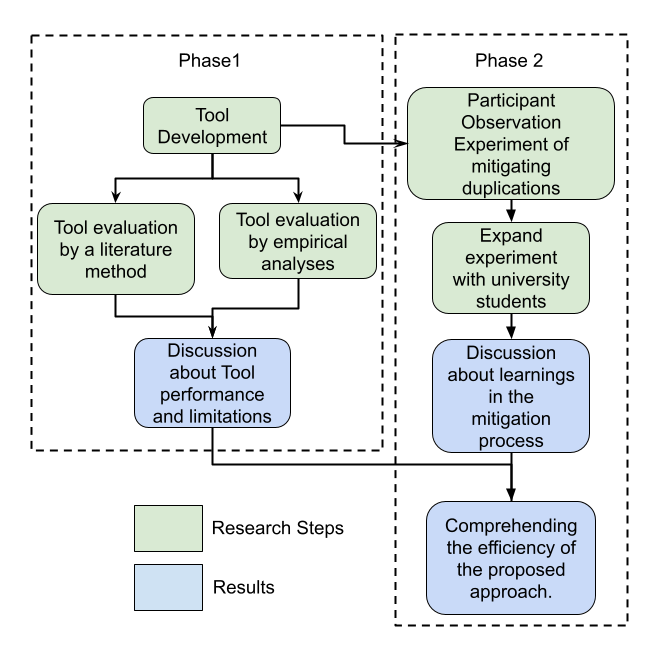
\includegraphics[scale=0.9]{research_design}
\caption{Diagram of the research design.}
\label{fig:reDesign}
\end{figure}

The initial phase of our research focused on the development and validation of ArKanjo, a 
command-line tool capable of identifying code duplication at the function level.  The 
tool's accuracy was rigorously validated by evaluating its performance against the 
standard BigCloneBench dataset \citep{bigclonebench} and by conducting an empirical analysis 
of its results within the AMD Display driver.  This foundational work ensured we had a 
reliable instrument to proceed with the practical investigation of code duplication 
in our target subsystems.

With a validated tool, the research then moved from detection to practice, investigating 
the real-world challenges of mitigating the identified duplications. This was accomplished 
through an ethnographic study designed to engage with the kernel community and understand 
their perspectives on code quality and refactoring.  This study had two components: a 
participant-observation experiment where the author submitted refactoring patches to the 
AMD Display driver, and a non-participant observation of university students using ArKanjo 
to contribute fixes to both the AMD Display and Industrial I/O subsystems.  

By combining tool 
development with direct community interaction, this research design allows for a comprehensive 
understanding of the technical and social factors that influence the mitigation of duplicated 
code in a large-scale open-source project.

\section**{Thesis Structure}

This manuscript consists of five more chapters. Chapter \ref{cha:back} presents
the literature overview for code duplication detection (main definitions,
current approaches in the literature), a brief description of the Linux kernel and the components
explored in this work, 
and a review of refactoring methods used throughout this research. Chapter
\ref{cha:tool} presents ArKanjo, our proposed tool to detect code duplication, 
describing all the main components.  Chapter \ref{cha:method}
describes the research methods selected to guide our work. Chapter
\ref{cha:results} shows the results we had through our work, from the research methods to 
evaluate our tool and the ethnographic studies. Chapter \ref{cha:conclusion} concludes this research.


\pagestyle{mainmatter}
%!TeX root=../tese.tex
%("dica" para o editor de texto: este arquivo é parte de um documento maior)
% para saber mais: https://tex.stackexchange.com/q/78101

\en

\chapter{Background}
\label{cha:back}

\en

This chapter presents an overview of fundamental topics needed to understand 
the research, such as the Linux Kernel, refactoring, types of code duplication, 
code duplication detection methods presented in the literature and ways to 
evaluate these methods. This foundation will make it easier to grasp the 
concepts discussed in the research.

\section{The Linux Kernel}

The Linux kernel, a Unix-like operating system kernel, was published by Linus
Torvalds in 1992 as free software. It began gaining popularity in the late
1990s \citep{linuxbook}. Contrary to popular belief, Linux itself is not a
complete operating system, as it lacks components like filesystem utilities and
windowing systems. The so-called ``Linux distributions'' that are commonly
recognized by the public are actually GNU/Linux operating systems, which
include various essential applications alongside the Linux kernel,
such as system
\citep{gnuref}. Examples of Linux distributions are Ubuntu \citep{ubuntu} 
and Arch Linux \citep{archlinux}.

The Linux kernel is monolithic and organized into subsystems, such as
the process scheduler, memory management, device driver infrastructure,
networking, and filesystems \citep{melissa}. Each subsystem typically has a
dedicated maintainer or a team of maintainers responsible for overseeing its
development and managing contributions \citep{melissa}.

Development contributions to the Linux kernel are coordinated using the Git
version control system. These contributions are formatted as patches—text
documents that outline the differences between two source code versions.
These patches are then submitted and reviewed via the Linux mailing lists
\citep{melissa}.

Mailing lists are the primary means of communication within the Linux
community. Members of the community use them to submit and review patches,
discuss Linux-related topics, and debate potential new features. Given the
kernel's extensive modularity, each subsystem has its mailing list, allowing
discussions to be organized around specific areas of development
\citep{melissa}. All interactions on these mailing lists are documented and
archived in the Linux Kernel Lore \citep{linuxlore}, which serves as a
repository for kernel discussions and can be accessed by anyone interested.

One of the subsystems within the Linux kernel is the AMD Display driver, which
is responsible for implementing the drivers needed for AMD GPUs to function
correctly in a Linux environment. The maintainers of this subsystem have
reported a practical issue: a significant amount of duplicated code, which
complicates the maintenance of this subsystem. This problem serves as the
starting point for our research, with the AMD Display driver as our primary
object of study as we aim to understand and mitigate code duplication in the
Linux kernel. The AMD Display driver subsystem contains more then 391000 lines 
of code and more then 1089 code files
\footnote{ 
Data extracted directly from the Linux repository with the help of the cloc tool.
\citep{cloc}
}, 
making it a considerable component within the Linux kernel. Like other 
subsystems, discussions about the AMD Display driver are conducted on its 
designated mailing list, which can be accessed here: 
\url{https://lists.freedesktop.org/mailman/listinfo/amd-gfx}.

Another subsystem within the Linux kernel explored in this work is the
Industrial I/O subsystem (IIO). According to the Linux kernel documentation, 
''The main purpose of the Industrial I/O subsystem (IIO) is to provide support 
for devices that in some sense perform either analog-to-digital conversion (ADC) 
or digital-to-analog conversion (DAC) or both''\citep{iiodoc}. The IIO subsystem 
contains more than X lines of code and more than Y code files
\footnote{
Data extracted directly from the Linux repository with the help of the clol tool. \citep{cloc}
}.
We opted to include the IIO subsystem in our experiments to ensure our findings 
are not limited to one subsystem. Additionally, we have an established point of
contact within the IIO subsystem to facilitate this work.
Like other subsystems, discussions about the IIO subsytem are conducted on its 
designated mailing list, which can be found here: 
\url{https://subspace.kernel.org/vger.kernel.org.html}.


\subsection{Diff command}

The \textit{diff} command is a command line in Linux that allows the user to compare 
two files line by line \citep{diffcommand}. There are multiple forms in which the command 
results can be shown to the user, and Figure \ref{fig:diff} shows one of them. 
With the command results, it is easy to visualize and extract the number of lines that 
are equal and different between the two compared files.

\begin{figure}
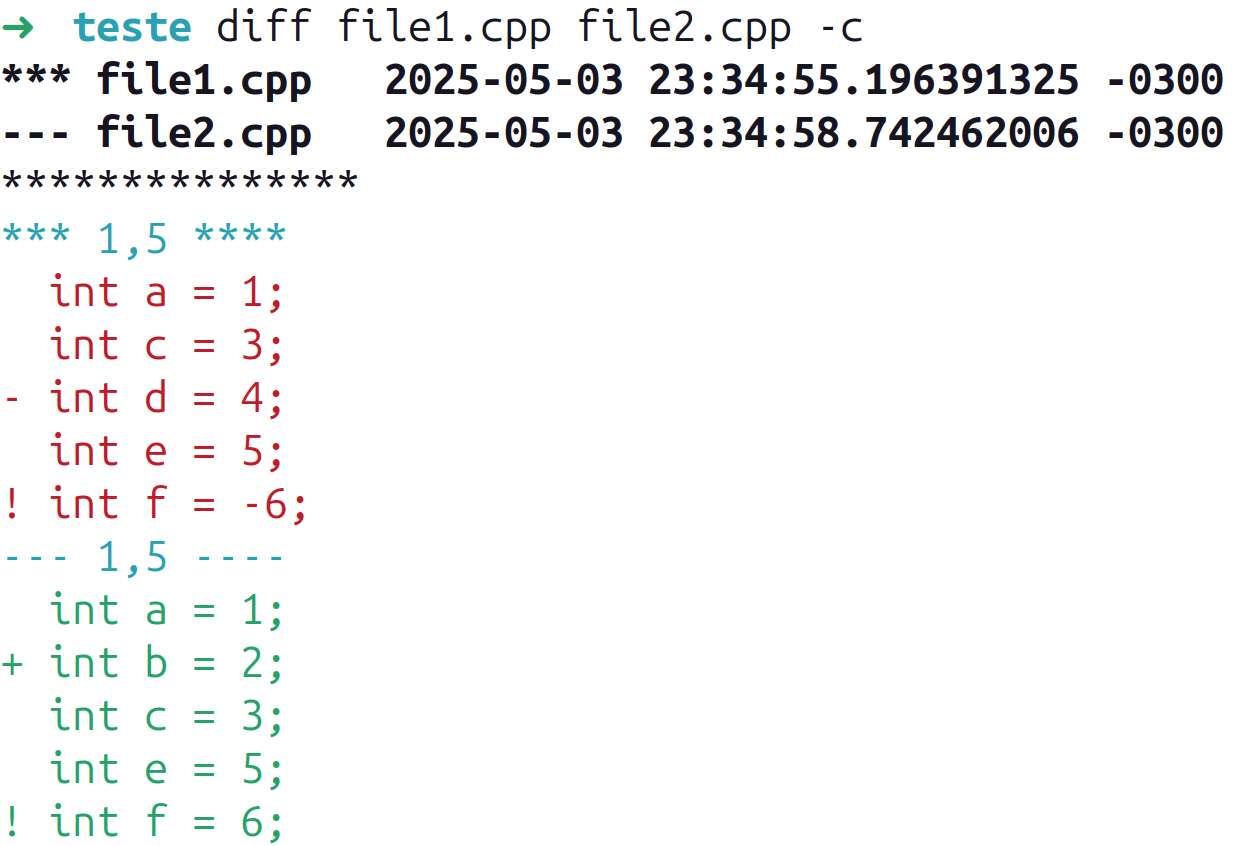
\includegraphics[scale=0.25]{diff_command}
\caption{Example of \textit{diff} command executed}
File 1's content is shown in red, and file 2's content is shown in green. \textit{-} 
represents a line that only exists in file 1, \textit{+} represents a line that only 
exists in file 2,\textit{!} represents a line that exists in both files but has modifications 
between them, and empty at the start of a line represents that the line exists in 
both files without any modifications.
\label{fig:diff}
\end{figure}

We use the \textit{diff} command as the base of one of the code duplication detection 
methods on the tool proposed in this work, although it is not explored as the text 
similarity method for code duplication detection.

\par
\en

\section{Code Duplication Detection}

Code Duplication Detection is a field in computer science studies that gets the attention of researchers 
back to 1988 \citep{firstman}.
The occurrence of Code Duplication is a harmful artifact to have in a software, affecting software related 
tasks such as code readability,
introdution of bugs, etc.   \citep{harmone}. 
On most of the cases, the occurrence of code duplication tends to create a more unstable software then the 
nonduplicate code counterpart.   \citep{harmtwo}

Through the years, the subject of studies about Code Duplication Detection branched out mainly in two fields of study,
Code Clone Detection and Code Plagiarism Detection,
with the former one focused on the technical aspect while the later one also introduces an social aspect on the field of research
\citep{litreview}. For our research we are only interested on the Code Clone Detection branch given the nature of our work.

\subsection{Types of code clone duplication}

\label{subsec:types}

The categorization of two code artifacts as a duplication of each other is a subjective task (REFERENCE HERE). 
To mitigate this human aspect on the given problem, the literature classified code duplication on the scale of changes between 
the code artifacts in four main types of code clone duplication \citep{litreview}. Given two code artifacts F and G, 
the types of Code Duplication are described as follow \citep{litreview}:

\begin{itemize}
	\begin{item}
		\textbf{Type-1:} The differences between F and G are in the context of revision of comments, variable names, white spaces 
		and any other kind of irrelevant elements. (ADD FIGURE) shows a typical example of Type-1 Code 
		Duplication \citep{litreview}. 
	\end{item}
	\begin{item}
		\textbf{Type-2:} The differences between F and G is the same as the type-1, with the addition of considering 
		addition and deletion of redudant codes. (ADD FIGURE) shows a typical example of Type-2 Code Duplication \citep{litreview}. 
	\end{item}
	\begin{item}
		\textbf{Type-3:} The difference between F and G is the same as the type-2, with the addition of considering 
		the reorder of code blocks as well as statements within code blocks. (ADD FIGURE) shows a typical example of 
		Type-3 Code Duplication \citep{litreview}. 
	\end{item}
	\begin{item}
		\textbf{Type-4:} The difference between F and G is the same as the type-3, with the addition of considering 
		changes on data sctrucure, the order of operands/operators in expresssions, or replacing part of codes with 
		equivalent composition. (ADD FIGURE) shows a typical example of Type-4 Code Duplication \citep{litreview}. 
	\end{item}



\end{itemize}

\subsection{Literature approches for code clone detection}

Given the passage of time, the literature developed many techniques and methods to approach the code clone detection problem. 
For better understanding and analyze of these approachs, the literature divided the researches done in
five main methodologies given the main nature of their work \citep{litreview} , which are:

\begin{itemize}
	\item \textbf{Textual-based approaches:} The literature review made by Chen \citep{litreview}  states that this methodology
	is the first to be investigated by the literature. This line of methodology is based on see code as a text artifact and apply
	textual approachs for text similarity. One example of this methodology applied is the work of Roy and Cordy \citep{textexample}, 
	which uses parsing and grammar techniques to detect code clones.

	\item \textbf{Token-based approaches:} This methodoly tries to approach the problem by seeing the code in a similar way to
	the lexical analysis of the compiling process \citep{litreview} . That means doing work in the line of recognizing constants, keywords and other 
	specific programming languages tokens, mapping variables to <pair,value> representations to become naming-independent, etc. One example of 
	this methodology applied  is the work of Toomey et al. \citep{tokenexample} to detect code clones through hashed token sequences.

	\item \textbf{Tree-based approaches:} While the token-based approach uses the lexical analysis of the compiling process, the 
	tree-based approach uses the syntax tree, the structure that  stores the semantic information of a code artifact in respect of the 
	programming language \citep{compiler}. One example of research that uses this information to detect code clones is the one done by
	Chilowicz and Duris \citep{treeexample}.

	\item \textbf{Metric-based approaches:} This methodology approches the problem by extracting metrics from the code artifact and use 
	those metrics as a embedding representation of the artifact to measure similarity \citep{litreview}, similarly to the famous  
	Word2Vec work done by Mikolov et al \citep{wordtovec}. Examples of metrics can be program size, number of variables, number of 
	access to memory, etc. One example of this methodology applied is the work done by Kaur and Sharma. \citep{metricexample}

	\item \textbf{Graph-based approaches:} Similarly to the Tree-based approaches, this methotodology depends heavily on an intermediate
	program representation, called program dependence graph (PDG) \citep{prodg}. The representation store information 
	about program's control, statement and data dependencies. One example of usage of the program dependence graph is 
	the recently work done by Liu et al. \citep{tailor}.
\end{itemize}

The state-of-art methods for code clone detection usually have high computational time and memory space usage, as well being
programming language specific approches, which cannot be easily implemented in programming languagues that were not used in 
their research \citep{litreview}. These are main concern for our research and for this reason we will use a generalist textual-based 
approach based solely on Natural Languague Processing (NLP) text similarity detection methods, which we will introduce and compare
with the literature approches later on this document. 

\subsection{Methodology to evaluate code duplication methods}

\label{subsec:codemethods}

Given the necessity to evaluate and compare approches for code clone detection, it was developed and widely-adopted two datasets: 
OJ-Clone, a dataset collected from a pedagogical online judge system \citep{ojclone}, and BigCloneBench, a dataset collected from over 
25,000 Java software systems \citep{bigclonebench}. The existence of only two spreaded datasets is a open concern in literature as 
the limited scope of OJ-Clone and the problems of BigCloneBench presented by Krinke and Ragkhitwetsagul \citep{bigfail}

(ADD INFORMATION ABOUT THE MORE SEPARATION OF CLONE TYPES THE BIGCLONEBENCH makes)












\par
\en

\section{Text Similarity Detection Methods}
\label{sec:similarity}

The standard methodology for text similarity detection is based on building
vector embeddings of texts and applying a distance function to these embeddings
to measure their similarity. The literature proposes multiple vector
embedding methods, such as bag-of-words, TF-IDF, LSI, and
Word2Vec~\citep{gensimlivro}. Recent works related to vector embedding construction
utilize Large Language Models (LLMs), as exemplified by Ethayarajh's work,
which employs BERT, ELMo, and GPT~\citep{llmsimilar}. The most popular distance
function used in the literature is cosine similarity, defined by the formula~\citep{cosineref}:

$$\text{cosine similarity} = SC(A,B) = \frac{ A \cdot B}{ \lVert A \rVert \lVert B \rVert }$$

Where $A$ and $B$ are the vector embeddings of the two texts. An advantage of
cosine similarity is that $SC(A,B)$ produces a number between $0$ and $1$,
where values closer to $1$ indicate higher similarity. It is common to
interpret cosine similarity as an approximation of probability, transforming
values between $0$ and $1$ into percentages between $0\%$ and $100\%$.
Throughout our research, we will use this percentage form.

It is well-known that LLMs have a high computational cost. For instance, an
analysis by Reimers and Gurevych found that finding the most similar pair in a
collection of 10,000 sentences required about 65 hours with
BERT~\citep{bertsimilar}. Since we aim to compare pairs of similar magnitude in
our work, we decided not to use LLMs for our vector embedding method, even
though they may be suitable for smaller codebases.

\subsection{Gensim}

Gensim is a FLOSS Python library~\citep{gensim}, which its creators
describe as ``The fastest library for training of vector embeddings -- Python or
otherwise. The core algorithms in Gensim use battle-hardened, highly optimized,
and parallelized C routines''~\citep{gensimsite}. Due to Gensim speed, we
chose this library for our vector embedding method.

In this work, we do not explore further alternatives for vector embeddings, as
optimizing computational cost or achieving state-of-the-art code clone
detection is not the primary objective of our research.

\par
\en

\section{Refactoring}

Fowler defines refactoring in his book as "a controlled technique for imporving the design of an existing code base. Its
essence is applying a series of small behavior-preserving transformations, each of which too small to be worth doing. However
the cumulative effect of each of these transformations is quite significant." \citep{refactorbook}. The elimination of detected 
code clone duplication is a refactoring task that necessitates the application of refactoring methods. 
Fowler presents multiples refactoring methods such as parameterize method, replace parameter with explicit methods and 
replace parameter with method \citep{refactorbook}. There is a briefly explanation of the methods used in our research below.

\subsection{Parameterize method}

TODO. I EXPECT TO FILL THIS SECTION AS THE WORK EVOLVES.

\par
\chapter{Proposed tool}
\label{cha:tool}

\en

Arkanjo, our proposed tool, is a Command Line Interface (CLI) application designed to
help developers identify code clone duplication at the function level.
Specifically, it enables the detection of pairs of functions within a codebase
that are clones of each other.

The tool operates in two main parts, the \textbf{Preprocessor} and the \textbf{Query Responder}. 
The \textbf{Preprocessor} is responsible to perform the heavy computations to find the code duplications 
accross a codebase and produce artifact to consulte information related to the duplications in a structured form.
The \textbf{Query Responder} consumes the artifacts produced by the Preprocessor to execute the tool functionalites as requested.
This choice enable the tool to concentrate the heavy and slows parts that can be execute only once per codebase, 
thus allowing a fast performance for multiple queries related to a single codebase.
More detailed descriptions of the Preprocessor and Query Responder can be found in
Sections \ref{subsec:architecture} and \ref{subsec:func}.

The Arkanjo tool has been implemented and is available for reference at
\url{https://github.com/LipArcanjo/arkanjo}.

\todo[inline]{Big maybes: Describe more how the functionalites are implemented, as the focus shifted for the tool as of now.}

\par
\en

\section{Tool architecture}
\label{subsec:architecture}

The Preprocessor contains two main components, the Function Breaker and the Code Duplication Finder. 
The flow of how the Preprocessor works is as follows: Function Parser receives the codebase the user is interested in,
extracts the functions of the codebase along with metadata, and creates a new temporary codebase where the functions extracted become new code files. 
The Code Duplication Finder iterates over every pair of files in the Temporary Codebase, checks if they are code clones, and, 
if so, saves them in the Code Duplication Database, which is a text file that stores every code duplication as a triple 
\textbf{<function1,function2,similarity>}, where \textbf{function1} and \textbf{function2} are the functions that are duplicates 
of each other, and \textbf{similarity} is the metric given by the code duplication detection method utilized in the Code Duplication Finder.

The Query Responder consumes the Temporary Codebase and the Code Duplication Database to extract duplicated 
functions-related information per user request. If the user executes the Query Responder without executing the 
Preprocessor, the Query Responder calls the Preprocessor to create the required artifacts.

Figure~\ref{fig:diagram} illustrates the tool architecture. An explanation of how each component works is provided in this section.

\begin{figure}
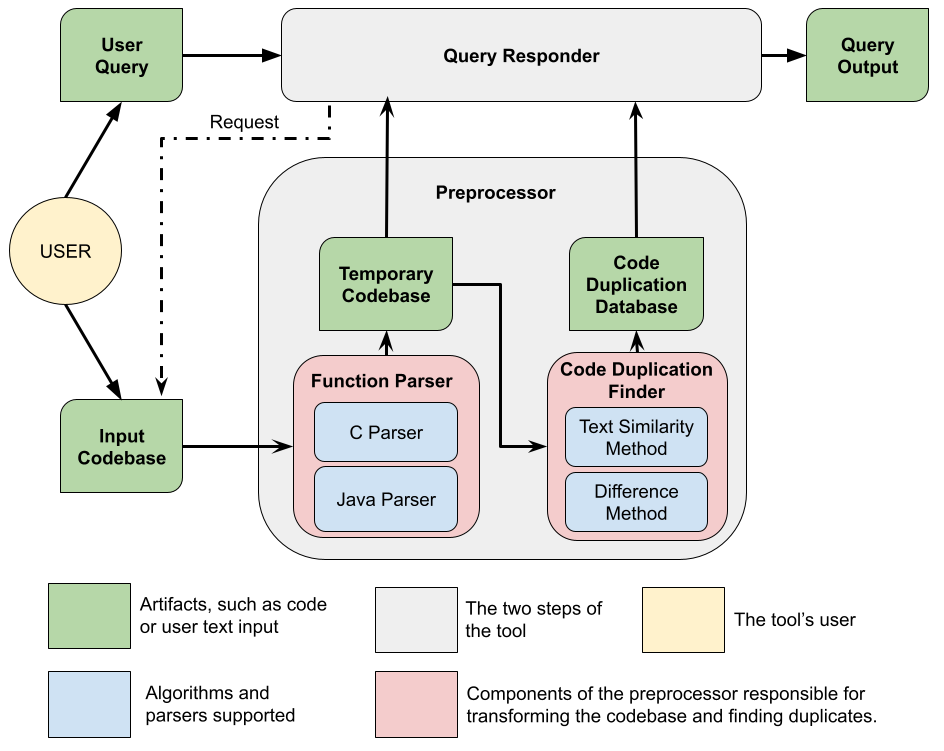
\includegraphics[scale=0.4]{diagrama_mestrado}
\caption{Architecture diagram demonstrating the relationship between the tool components.}
\label{fig:diagram}
\end{figure}

\subsection{Input codebase}

The input codebase is a folder on the machine running the tool. All files in the codebase that are not source code files from a programming language supported by the tool are ignored. The tool validates support for a source file by analyzing its file extension.

\subsection{Function Parser}

The Function Parser receives the input codebase and transforms it into the temporary
codebase. It iterates through every source code file written in a supported programming 
language and uses a language-specific extractor to isolate each function. For each extracted 
function, two new source code files and a metadata file are created in the temporary codebase, 
represented by the pair \textbf{$<$file name, function name$>$}, the source code of the function, 
and the function metadata (in practice, this is a duplication of the original codebase, 
structured as a parsed representation). One of the new files contains the function body, and the other 
contains the function signature. The metadata file includes additional relevant information,
such as the function name, the line where the signature starts, and the line where the function 
body ends. Currently, the supported programming languages are C and Java, although Java support is limited.

\begin{figure}
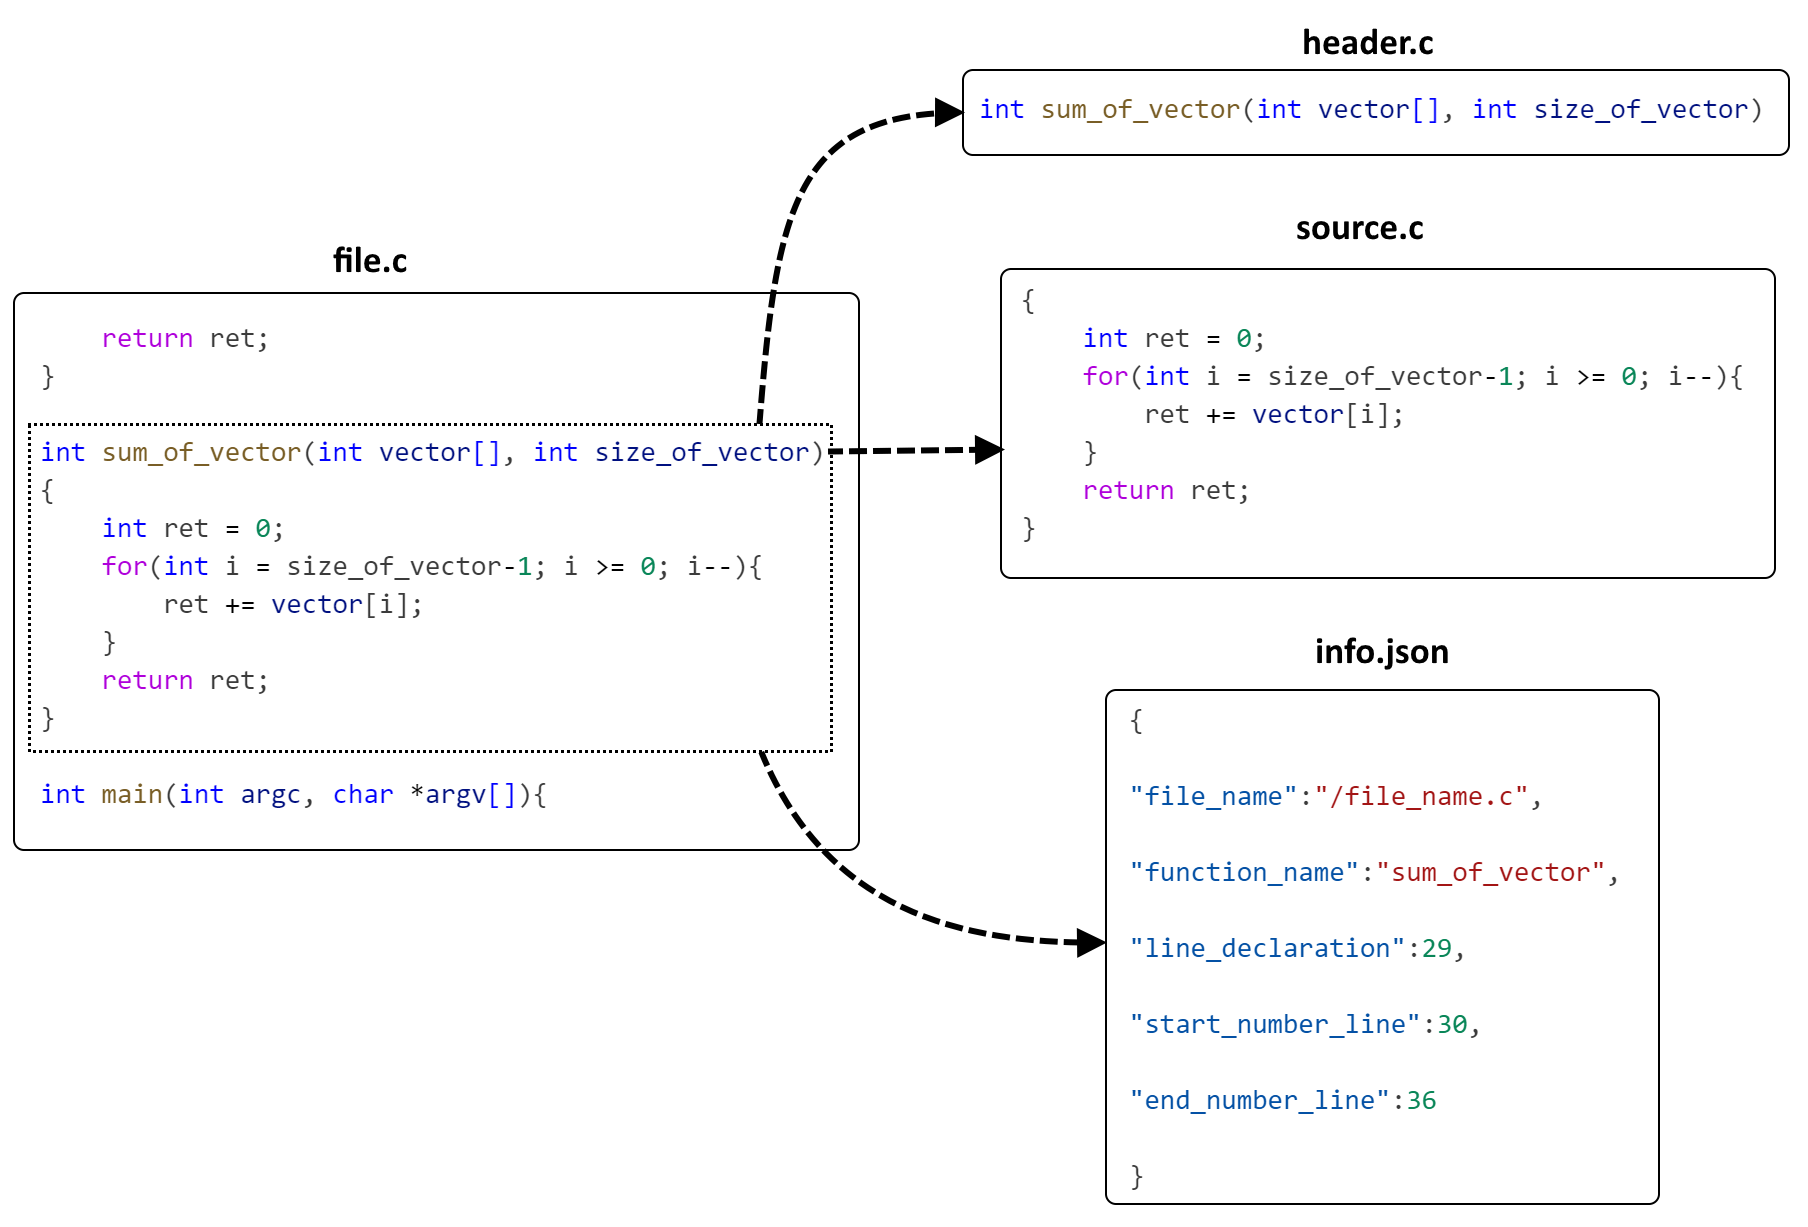
\includegraphics[scale=0.3]{example_function_parser/example_parser}
\caption{Transformation of a function into the temporary codebase}
\label{fig:transform}
\end{figure}

Regarding the programming language function extractor, we approached this problem so that anyone 
comfortable with a language can adapt our approach to their specific programming language. 
Usually, code blocks can be easily extracted from source code files, independently of whether the 
code blocks are defined by curly brackets or by indentation, and it is possible to infer if 
they represent a function body given their depth in the code context and a few lines before the 
start of the code block. We followed this approach to implement the function extractor for the 
supported languages. As an alternative approach, we can build the syntax tree~\citep{compiler} 
of the programming language and use it to extract the functions, which is a more complex task than 
our approach. For the programming languages that we support, we implemented them as follows:

\subsubsection{C Programming Language}

For a source file in the C programming language, we extract the code blocks with depth 0. 
As per the programming language grammar, functions are defined in a global context at depth 0. 
To extract the code blocks, we first need to identify the portions of code that are comments or 
\textit{\#define} directives and mark them as irrelevant. After that, it is simple work to find 
the curly brackets in depth 0; with that, we find the body of the functions.

To extract the header of the functions, we start at the open curly brackets and go back in the 
source file, considering the programming language grammar and the portions of code 
marked as irrelevant because of comments and \textit{\#define} directives.
Other elements in depth zero are not functions; we analyze whether the code blocks 
are functions at the same time that we extract the header of the code block.

\subsubsection{Java Programming Language}

For the Java programming language, we have decided to implement a more straightforward approach 
that does not support the programming language completely, as the only Java codebase explored in 
this work is the BigCloneBench~\citep{bigclonebench}, and the approach implemented covers the 
needs of this codebase.

We extract the code blocks with depth one and some code lines for a source file in Java before 
defining them. Then, we check if the code blocks are functions by analyzing whether the first 
non-empty character before the curly brackets of the code block is a closing parenthesis.

As per Java grammar, functions are defined inside classes and can exist at different depths. 
As Java accepts inner classes, this approach does not work with inner classes. The challenge 
to implementing a more generic approach is that other elements of depth two or deeper, such 
as for-loops, can follow the closing parenthesis pattern, necessitating a better analysis of 
these elements. The BigCloneBench~\citep{bigclonebench} does not contain inner classes.

\subsection{Temporary codebase}

The temporary codebase is a transformation of the input codebase performed by the Function Parser. Each function in the input codebase is represented in the temporary codebase as three files. Descriptions of these files are provided below, with examples shown in Figure~\ref{fig:transform}.

\begin{itemize}
	\item \textbf{Header file}: This file contains the signature of the function it represents.
	\item \textbf{Source file}: This file contains the body of the function it represents.
	\item \textbf{Info file}: This file contains metadata about the function, including the function name, the file that contains the function, the file relative path to the input codebase, the line where the function signature starts, the line where the function body begins, the line where the function body ends, and whether there is a line break between the end of the function signature and the start of the function body.
\end{itemize}

\subsection{Code Duplication Finder}
\label{subsec:code_finder}

The Code Duplication Finder iterates through every pair of source code files in the temporary codebase, representing functions from the input codebase. For each pair of files, we execute a code duplication detection method that computes a metric measuring how similar the pair of files is, which we refer to as similarity. 
If the similarity is greater than or equal to the minimum similarity threshold 
(a parameter provided by the user during the Preprocessor). We store this pair of functions and its 
similarity in the Code Duplication Database.

We implemented two methods for code duplication detection in the tool, which the user can 
use. The first method is based on text similarity, and the second is simpler and 
based on the number of equal lines. The experiments and tests in this research were done 
using the text similarity method. The purpose of the second method is to demonstrate that 
the tool can have multiple duplication detection methods.

\subsubsection{Text Similarity Method}

For the text similarity method, we treat the source code files 
as text and apply the TF-IDF vector embedding method implemented by the 
Gensim library~\citep{gensim}, then compute cosine similarity as the 
similarity metric.

We chose this method for its claimed performance, 
programming language independence, and the fact that it does not require 
compilable code, which is expected in the temporary codebase, as it does 
not contain complete code artifacts. We expect our method to yield good 
results for Type-1 and Type-2 code duplication types while performing 
poorly for others. Changing the code duplication
detection method to one of the state-of-the-art methods is possible if needed.

\cite{platistool} implemented this code duplication detection method and 
released it under the MIT license. We adapted his 
implementation to fit our tool expected input and output formats. 
Switching the duplication detection method is feasible, similar to how 
we adapted Plates' implementation.

\subsubsection{Difference Method}

For the difference method, 
we implemented a method that considered the number of exactly equal lines between two functions.
For two functions \textit{function1} and \textit{function2}, let $NL_1$ be the number of lines in \textit{function1},
$NL_2$ be the number of lines in \textit{function2}, and $EQ$ be the number of equal lines between \textit{function1} and
\textit{function2}, we compute the similarity with the formula:

$$\frac{2 \cdot EQ}{NL_1 + NL_2}$$

This code duplication method is considerably simpler and more explainable than the text similarity method, 
as the metric is the ratio of common lines between the two functions. 
We use the \textit{diff} command built-in the Linux environment \citep{diffcommand}
to compute the number of equal lines.

We did not test the Diff method during the tool evaluation and other phases of this research. 
We implemented the technique to show that a tool can have multiple duplication detection methods.

\subsection{Code Duplication Database}

The Code Duplication Database is a text file that contains the duplicated pairs of functions found by the Code Duplication Finder. The first line of the file specifies the number of duplicated pairs. Following this, each line lists a duplicated pair, including the paths of the functions in the temporary codebase and the similarity metric of the pair.

\subsection{Preprocessor}
\label{subsec:setup}

The Preprocessor is a procedure executed by the user once per codebase. 
The Preprocessor takes the input codebase and a minimum similarity metric value for function pairs considered duplicates. 
It then runs the Function Parser and the Code Duplication Finder to create a temporary codebase and the Code Duplication Database. 
Setting a minimum similarity metric reduces the Code Duplication Database size, optimizing memory usage and the computational 
cost of the Query Responder step. For example, if this parameter does not exist and we work with a codebase of $10,000$ functions, 
each with a 50-character relative path and function name, the Code Duplication Database would reach approximately $5,000^2 \times 50 ~= 5$ gigabytes. 
As most function pairs are unlikely to be duplicated in large codebases, this file size can be significantly reduced.

\subsection{Query Responder}

The Query Responder step is the component that the user executes multiple times to consult information 
about duplicated functions in a codebase processed by the Preprocessor. 
It utilizes the Temporary Codebase and the Code Duplication Database as inputs to answer user requests, 
such as querying for duplicated functions above a certain similarity threshold or providing counts of such functions.
This component was developed to be extensible, allowing other query functionalities to be easily added. 
The specific functionalities provided to the user by the Query Responder, which include the 
Duplication Explorer, Function Information, and Duplication Report, are described in Section~\ref{subsec:func}.


\par
\en

\section{Tool functionalites}
\label{subsec:func}

We proposes three main functionalities for the user in the tool, which are named duplication explorer, function information
and duplication relatory. Each of the functionalities recevies their adequated parameters to execute, with a exception
of a optional parameter shared by all of them, which is minimum similarity per query. The minimum similarity per query is different
from the siminum similarity presented in \ref{subsec:setup}, as it enables a volatile change in the minimum similarity
interested in a query specific context. There is a explanation of each of the main functionalities throughout this section.

\subsection{Duplication explorer}

The duplication explorer is the principal functionality of our tool, the functionality purpose is to expose for the user the code duplication
pairs found by our tool. We implement optional filters methods to enable more complex queries, which are described below. A example
of the functionality usage can be found in (ADD FIGURE HERE).


\begin{itemize}
	\begin{item}
		\textbf{Sorting filter:} This filter enables the user to sort the resuls by similarity of the functions pairs or 
		by the number of duplicated lines. By default the tool sorts by similarity and the user can pass a sort parameter to change
		the sorting method.
	\end{item}

	\begin{item}
		\textbf{Limiter filter:} This filter receives a number parameter named limiter by the user, which limits the number of results
		showed to the user by this given number.
	\end{item}

	\begin{item}
		\textbf{Pattern Filter:} This filter make the explorer ignore every pair of duplicated functions that does not match a pattern
		given by the user as a parameter. We say that a function matches a pattern if the string formed by the concatenation of
		the relative path of the code file plus the function name. The user can define if both functions or at least one of the 
		functions in the pair need to match the pattern by given a specific parameter.
	\end{item}
\end{itemize}


\subsection{Function information}

The Function information purpose it to give a more in depth information about a specific function. The functionality inform the user
about the relative path, the function name and the lines the function exist in the code file that the function is contained for the
function that the user is interested and every function that is a duplication of it. As there ca nbe multiple functions with the 
same name in a codebase, we distinguish then by the user providing a pattern string and we use the first function find that match
the pattern. We say that a function matches a pattern if the string formed by the concatenation of the relative path of the 
code file plus the function name. 
A example of the functionality usage can be found in (ADD FIGURE HERE).

\subsection{Duplication relatory}

The duplication relatory purpose is to give a overview of the input codebase. The functionality extract the information
of how much lines of duplicated code is found per folder in the codebase and present it to the user in a reasonable format. To extract
the information, we use the Code Duplication Database to list the code duplications, and the temporary code to know how much lines of
duplicated code contains in each of the functions. (DO I TALK ABOUT THE TRIE USAGE TO MAINTAIN THE HIERARCHICAL TREE STRUCTURE? I 
THINK NOT). A example of the functionality usage can be found in (ADD FIGURE HERE).






\par

\chapter{Research Methods}
\label{cha:method}

We employ a multi-method research approach, using different methodologies to achieve our goals
to approach code duplication in some of the Linux subsystems. 
To validate if the Arkanjo tool is capable of finding code duplications, 
applied two independent methods and perform triangulation on the results. 

The first method evaluates the proposed tool using an approach from the literature, 
comparing it against the BigCloneBench dataset \citep{bigclonebench}. 
The second method is an empirical analysis of a subset of functions within the 
AMD Display driver that our tool identified as duplicates. After completing these two 
methods, we triangulated the findings to analyze the results comprehensively. 
We chose triangulation because relying solely on the literature-based method has 
limitations and may not be entirely reliable \citep{bigfail, litreview}. As a reminder, 
all research approches were done using the text similarity method as the 
code dupication method of the tool.

Given the validation of the tool's capabilities, we proceed to undertand the viability 
to mitigate the code duplication finds by the tool. 
To underdand the viability, our first choice is to conduct an ethnographic study using 
a participant-observation methodology. 
In this study, we aim to mitigate a subset of duplicated functions by refactoring them 
while interacting with the Linux community to gather feedback on our mitigation efforts. 

The ethnographic study happened in two phases. 
In the first phase, the author of this research explored the process of mitigating
a code duplication found in the AMD Display Driver and sent it as a PATCH to iteract with the
Linux community and get their feedback. On a second phase, we proposed to students on the 
course Free Software Development at University São Paulo to mitigate the code duplications found 
by the tool in the IIO and AMD Display Driver and pass the process of send the mitigations as PATCH.
(DOUBLE CHECK IF THE STUDENTS HAVE SENT THE PATCHES). 

I 

\todo[inline]{The focus of the above section should be a little more on the tool, the introduction about mitigating duplications is good enough. A little about the fact that we will test on IIO later maybe is good. }

\todo[inline]{I SHOULD mention that the test on the tool were made using the gensim similarity method and not the git method.}

\section{Evaluation of the Tool by the BigCloneBench dataset}

\label{sec:metbig}

The BigCloneBench dataset \citep{bigclonebench} is a Java code collection containing pairs of code duplications categorized by clone type, as defined in Section \ref{subsec:types}.
%
Following the methodology presented by \citep{tailor}, we sampled 20,000 pairs from each clone type, adding 20,000 non-duplicate pairs as negative samples. We applied the same sampling approach to our tool to ensure a fair evaluation.

Unlike traditional methods, our tool does not distinguish between clone types and identifies duplications at the function level rather than the file level, which is typical in state-of-the-art tools. Therefore, we adapted the metric calculation method for evaluation purposes. Specifically, we considered every pair of functions with a similarity metric equal to or greater than a threshold \(X\) as duplicates and marked the corresponding file pairs. A correctly identified duplication pair counts as accurate for its clone type, while an incorrectly inferred pair is considered incorrect across all clone types. With these definitions, we computed the Recall metric from Section \ref{subsec:codemethods} for each clone type.
%
To understand the impact of varying the similarity threshold, we evaluated our tool using different threshold values: 30\%, 40\%, 50\%, 60\%, 70\%, 80\%, 90\%, and 100\%. We then analyzed and discussed the results.

\section{Evaluation of the Tool by Empirical Analysis}

\label{sec:metemp}

\todo[inline]{I just mention the problem, maybe a more explictly mention of the problem here or on the background would be good.}

Due to the limitations of the BigCloneBench dataset, as noted by \cite{bigfail}, and its lack of suitability 
for our context (Java dataset vs. C-based Linux kernel), we complemented the BigCloneBench evaluation with 
an empirical study of the tool inferred duplications.

%
Given the vast number of lines and components in the Linux kernel, analyzing every duplication is impractical. We focused our scope on the AMD Display driver, which, as shown in Figure \ref{fig:relatory_ex}, contains over 20,000 lines of duplicated code at a similarity metric of 100\%.

In this empirical analysis, we randomly sampled function pairs identified by the tool as duplicates. For each similarity threshold \(X\) (30\%, 40\%, 50\%, 60\%, 70\%, 80\%, 90\%, and 100\%), we randomly selected ten function pairs with a similarity close to \(X\), allowing for a 1\% deviation. We implemented the random selection using the tool's source code.

Appendix \ref{app:emp} lists the randomly selected function pairs. We empirically evaluated these pairs to determine if they were duplications, comparing these results with the literature-based method to assess our tool's effectiveness and understand the impact of the minimum similarity parameter.

\todo[inline]{Take care: Big focus on AMD display driver and the tone of the writing supports the focus. }

\section{Ethnographic Study}

\label{sec:meteth}

Ethnography is a recognized qualitative empirical method for understanding people, 
their cultures, and their work practices \citep{bookethno}. It allows researchers 
to gain insights into values, beliefs, and ideas from the perspective of community 
members \citep{ethnosoft}. In our research, refactoring code duplications without 
community interaction would prevent us from understanding whether Linux maintainers 
would accept our approach or identify their concerns. Thus, we will use ethnography, 
positioning ourselves as Linux kernel contributors focused on removing identified 
code duplications.

This section outlines our approach for mitigatin code duplication in the Linux kernel
and describes the ethnographic methodology for engagin with the Linux community. Firstly, 
we present the participant observation research method explored by the author. Then, 
we present the methodolody of the experiment done with the students.

\subsection{Participant observation method}


\subsection{Research with students}

\todo[inline]{Rsearch with students does not look good.}

In the Free Software Development course at University of São Paulo, ministred by the advisor 
of this work at the first semester of 2025, we have proposed to the students the possibility
of mitigating duplications in the IIO subsystem and the AMD display driver found with the Arkanjo tool.
The course had a total of X students, and of that, X students being undergraduate students
and Y begin graduate students.

On the course, the students are asked to form groups of one, two or three students and together 
make a contribution to a open source software. To auxiliate the students on this task, the 
professor and teaching assistants prepares multiple alternatives on how to contribute to open source projects, 
including simple contributions as updating documentation or code style fixes. In this context, 
we have proposed two alternatives for the students related to the tool.

For the first alternative, one of the teaching assistants used the Arkanjo tool in the IIO subsystem and
listed interesting duplications that the groups can approach, and it is up to the students on how
to refactor the code to mitigate the duplications and pass through the process to send patches to the IIO 
maintainers to review. For the second alternative, we propose a similar experience then the 
participant observation method, where the students pass through the whole process of executing the Arkanjo tool
in the AMD display driver, analyze the duplications found, create a patch to mitigate a duplication and sent
the patch to the AMD display driver's maintainers.

From the students enrolled in the in the course, X opted for the first alternative and 1 opted for the second
alternative, forming Y groups working on the first alternative and 1 group working on the second alternative. 
These number represent X\% of the students choosing for approching duplications them the other contribution 
alternatives, including more simpler and easy to be done.  It is worth highlighting that none of the students
that choose to mitigate duplications had made a contribution to the Linux kernel before,
meaning that the patch to mitigate the duplication being the first tentative to contribute to the kernel as
newcomers.

The groups have been request to document the experience and approaches to refactor the duplications and the
experience of submiting a patch to the Linux kernel in blogs. We had analyzed these blogs to undertand 
patterns of refactor used for mitigating the duplications, the experience on send the patches and the 
opinions of the subsystem maintainers on the mitigations. Appendix X list the blogs and patches made by the 
student.

For the teaching assistant and the student that has executed the Arkanjo tool to explore duplications, 
we have asked them to answer some questions related to the experience of using the tool and what could be
improved. The question asked can be found below and the answers can be found in Appendix Y.



\par

\chapter{Preliminar Results}
\label{cha:results}

\en

Base Content of the Preliminar Results of the research. TODO.




%!TeX root=../tese.tex
%("dica" para o editor de texto: este arquivo é parte de um documento maior)
% para saber mais: https://tex.stackexchange.com/q/78101

\chapter{Usando este modelo}

Não é necessário que o texto seja redigido usando \LaTeX{} ou este modelo,
mas seu uso é fortemente recomendado, pois ele facilita diversas etapas do
trabalho e o resultado final é muito bom\footnote{O uso de um sistema de
controle de versões, como mercurial (\url{mercurial-scm.org}) ou git
(\url{git-scm.com}), também é altamente recomendado.}. Este modelo é
distribuído com uma ``colinha'' dos principais comandos \LaTeX{} e
inclui comentários explicativos para auxiliá-lo com ele, sendo composto
pelos~arquivos:\looseness=1

\enlargethispage{-1\baselineskip}

\begin{itemize}
  \item \texttt{tese.tex}, \texttt{artigo.tex}, \texttt{apresentacao.tex}
        e \texttt{poster.tex} (exemplos de cada um desses tipos de documento);
  \item Capítulos, apêndices, imagens etc. deste texto de exemplo, nos
        diretórios \texttt{conteudo}, \texttt{figuras} e \texttt{logos}
        (procure os comandos \texttt{\textbackslash{}input} e
        \texttt{\textbackslash{}graphicspath} nos arquivos de exemplo
        mencionados acima para modificar o nome desses diretórios);
  \item \texttt{bibliografia.bib} (exemplo de banco de dados bibliográficos;
        procure o comando \texttt{\textbackslash{}addbibresource} nos
        arquivos de exemplo mencionados acima para modificar o nome desse
        arquivo ou acrescentar outros);
  \item \texttt{imegoodies.sty}, que carrega várias \emph{packages} comumente
        usadas. Você normalmente não vai precisar mexer nesse arquivo, mas
        pode fazê-lo se quiser, e também pode usá-lo em outros documentos
        \LaTeX{} (veja o Anexo~\ref{ann:imegoodlooks});
  \item \texttt{imelooks.sty}, que carrega mais \emph{packages} e define
        diversas opções relacionadas à aparência do documento, inclusive
        a capa da tese. Você normalmente também não vai precisar mexer
        nesse arquivo, mas pode fazê-lo se quiser, além de também poder
        usá-lo em outros documentos \LaTeX{} (veja o Anexo~\ref{ann:imegoodlooks});
  \item \texttt{evenragged.sty}, \texttt{froufrou.sty}, \texttt{lstpseudocode.sty},
        \texttt{texlogsieve} e \texttt{texlogsieverc} (classes e programas
        auxiliares ao modelo);
  \item \texttt{beamer-ime.[bbx|cbx]}, \texttt{plainnat-ime.[bbx|cbx]} e
        \texttt{plainnat-ime[-en].bst} (definições de estilos bibliográficos).
\end{itemize}

Para compilar o documento, basta executar o comando
\textsf{latexmk}\footnote{Você também pode usar \textsf{latexmk poster},
\textsf{latexmk apresentacao} etc.}. Talvez seu editor ofereça uma opção
de menu para compilar o documento; sempre que possível, configure-o para
utilizar o \textsf{latexmk} ao selecioná-la. \LaTeX{} gera diversos arquivos
auxiliares durante a compilação que, em algumas raras situações, podem ficar
inconsistentes (causando erros de compilação ou erros no \textsc{pdf} gerado,
como referências faltando ou numeração de páginas incorreta no sumário).
Nesse caso, é só usar o comando \textsf{latexmk -C}, que apaga todos esses
arquivos auxiliares gerados, e em seguida rodar \textsf{latexmk} novamente.

Você pode mudar a língua do documento para o inglês no início de cada
arquivo .tex de exemplo, na linha \textsf{\textbackslash{}documentclass}.
No caso do arquivo \textsf{tese.tex}, isso muda todos os textos padrão
da capa e folhas de rosto.

Os arquivos deste modelo incluem vários comentários com dicas e explicações;
se o que você precisa não está mencionado diretamente, é provável que haja
pelo menos a indicação da \textit{package} relacionada ao que você precisa.

Se você encontrar algum problema com o modelo, ajude a melhorá-lo!
Envie um relatório de erro ou entre em contato em
\url{gitlab.com/ccsl-usp/modelo-latex}.

%!TeX root=../tese.tex
%("dica" para o editor de texto: este arquivo é parte de um documento maior)
% para saber mais: https://tex.stackexchange.com/q/78101

\chapter{Instalação do \LaTeX{}}
\label{chap:install}

\LaTeX{} é, na verdade, um conjunto de programas. Ao invés de procurar e
baixar cada um deles, o mais comum é baixar uma coleção com todos eles juntos.
Há duas coleções desse tipo disponíveis: MiK\TeX{} (\href{http://miktex.org}
{miktex.org}) e \TeX{}Live (\href{http://www.tug.org/texlive}
{www.tug.org/texlive}). Ambos funcionam em Linux, Windows e macOS. Em Linux,
\TeX{}Live costuma estar disponível para instalação junto com os demais
opcionais do sistema. Em macOS, o mais popular é o Mac\TeX{} (\href
{http://www.tug.org/mactex/}{www.tug.org/mactex/}), a versão do \TeX{}Live
para macOS. Em Windows, o mais comumente usado é o MiK\TeX{}.

Por padrão, eles não instalam tudo que está disponível, mas sim apenas os
componentes mais usados, e oferecem um gestor de pacotes que permite adicionar
outros. Embora uma instalação completa do \LaTeX{} seja relativamente grande
(perto de 5GB), em geral vale a pena instalar a maior parte dos componentes.
Se você preferir uma instalação mais ``enxuta'', não deixe de incluir tudo
que é necessário para este modelo, como indicado no arquivo README.md.

Também é muito importante ter o \textsf{latexmk}. No Linux, a instalação
é similar à de outros programas. No macOS e no Windows, \textsf{latexmk}
pode ser instalado pelo gestor de pacotes do MiK\TeX{} ou \TeX{}Live.
Observe que ele depende da linguagem \textsf{perl}. No macOS, \textsf{perl}
já faz parte do sistema; no Windows, \TeX{}Live inclui uma versão básica
de perl, mas se você estiver usando MiK\TeX{} será preciso instalar
\textsf{perl} manualmente (\href{http://www.perl.org/get.html}
{www.perl.org/get.html}).

\section{Documentação sobre \LaTeX}
\label{sec:docs}

Há muito material sobre \LaTeX{} na Internet, mas também há muita informação
obsoleta (incluindo trechos da própria documentação oficial!). Em particular,
você pode ignorar explicações sobre como converter arquivos no formato
\textsc{dvi} gerados por \LaTeX{} em \textsc{pdf}: as versões atualmente
recomendadas de \LaTeX{} (cf. Seção~\ref{sec:versions}) geram arquivos
\textsc{pdf} diretamente. Quanto a imagens, os formatos de arquivo
\textsc{ps/eps} (PostScript e Encapsulated PostScript) não são adequados
para essas novas versões de \LaTeX{}; elas trabalham com arquivos de imagem
nos formatos \textsc{pdf}, \textsc{png} e \textsc{jpeg}. Finalmente,
recursos gráficos normalmente não usam mais \textit{packages} como
\textsf{pstricks}, \textsf{eepic} ou outras tradicionalmente citadas;
ao invés disso, \textsf{PGF/TikZ} é a ferramenta mais comum.

Como dito anteriormente, \LaTeX{} é, na verdade, um conjunto de programas
e, em geral, instalamos coleções pré-prontas com todos eles. Essas coleções
(\TeX{}Live e MiK\TeX{}) contêm também a documentação das \textit{packages}
incluídas: Basta digitar \textsf{texdoc nome-da-package} (\TeX{}Live) ou
\textsf{mthelp nome-da-package} (MiK\TeX{}) para ter acesso à documentação
correspondente. \textsf{texdoc/mthelp} incluem também alguns tutoriais e
textos introdutórios.

Um possível caminho para o aprendizado é começar com o
Capítulo~\ref{chap:tutorial} deste modelo e o conteúdo em
\href{http://overleaf.com/learn}{overleaf.com/learn}, que tem escopo similar
mas também inclui várias páginas sobre como utilizar recursos específicos.
Após esse contato inicial, o tutorial em \href
{http://tug.org/twg/mactex/tutorials/ltxprimer-1.0.pdf}
{tug.org/twg/mactex/tutorials/ltxprimer-1.0.pdf} é
bastante abrangente e detalhado. Não deixe de ver também o
Capítulo~\ref{chap:exemplos} deste modelo (e seu código-fonte), que
inclui várias dicas úteis. Para os principais comandos do modo matemático,
veja \textsf{texdoc undergradmath} e, para aprender a criar apresentações,
veja \textsf{texdoc beamer}.

Depois que você estiver razoavelmente
familiarizado com a linguagem, utilize o manual de referência que pode ser
acessado em \href{http://latexref.xyz}{latexref.xyz} ou com \textsf{texdoc
latex2e} (disponível também em francês, com \textsf{texdoc latex2e-fr.pdf}
e em espanhol, com \textsf{texdoc latex2e-es.pdf}).

A documentação de referência mais importante sobre os recursos matemáticos
é acessível com \textsf{texdoc amsmath}, \textsf{texdoc amsthm} e
\textsf{texdoc mathtools}; \textsf{texdoc maths-symbols} agrega os símbolos
matemáticos disponíveis. Para uma lista completa de todos os símbolos
disponíveis com \LaTeX{}, use \textsf{texdoc symbols-a4} (esse documento
tem mais de 300 páginas!).

Existem também diversos bons livros sobre \LaTeX{} (embora em geral um
tanto antigos), dos quais destacamos dois:

\begin{enumerate}

  % https://www.math.ucdavis.edu/~tracy/courses/math129/Guide_To_LaTeX.pdf
  % https://archive.org/details/a-guide-to-la-te-x-and-electronic-publishing/page/n7/mode/2up
  \item A quarta edição de ``A Guide to \LaTeX'', de Helmut Kopka
        e Patrick W. Daly (publicada em 2003), além de uma ótima
        introdução, aborda vários tópicos relativamente avançados
        e úteis\footnote{Uma versão não-final está disponível em
        \href{http://www2.mps.mpg.de/homes/daly/GTL/gtl\_20030512.pdf}
        {www2.mps.mpg.de/homes/daly/GTL/gtl\_20030512.pdf}.}.
  \item A segunda edição de ``The \LaTeX{} Companion'' (publicada em
        2004) é um livro quase obrigatório, pois discute em detalhes
        praticamente todos os recursos e \textit{packages} importantes
        de \LaTeX{}, servindo tanto para o aprendizado quanto como
        material de referência.

\end{enumerate}

Para dúvidas pontuais, o sítio \href{http://tex.stackexchange.com}
{tex.stackexchange.com} é um fórum de perguntas e respostas sobre
\LaTeX{} muito útil, pois os principais desenvolvedores do sistema
participam das discussões, e o sítio \href{http://texfaq.org}{texfaq.org}
é bastante abrangente e atualizado.

\froufrou

Existem inúmeras alternativas aos materiais citados acima; outros exemplos de
textos introdutórios são \href
{http://www.maths.tcd.ie/~dwilkins/LaTeXPrimer/GSWLaTeX.pdf}
{www.maths.tcd.ie/\textasciitilde{}dwilkins/LaTeXPrimer/GSWLaTeX.pdf} e
\href{http://www.andy-roberts.net/writing/latex}
{www.andy-roberts.net/writing/latex}. Em português, você pode
consultar \href
{http://polignu.org/sites/polignu.org/files/latex/latex-fflch.pdf}
{polignu.org/sites/polignu.org/files/latex/latex-fflch.pdf}
e \href{http://git.febrace.org.br/material-latex/material-latex}
{git.febrace.org.br/material-latex/material-latex} (este precisa ser
baixado e compilado). O canal \href{http://youtube.com/c/anteroneves}
{youtube.com/c/anteroneves} tem vários vídeos instrutivos em português.
\textsf{texdoc/mthelp} incluem ainda opções como ``The Not So Short
Introduction to \LaTeXe{}'' (\textsf{texdoc lshort-eng}; há uma versão
em português, mas não está em dia com o original) e ``A Simplified
Introduction to \LaTeX{}'' (\textsf{texdoc simplified-intro}). Versões
recentes do \LaTeX{} incluem também o ``\LaTeXe{} via exemplos''
(\textsf{texdoc latex-via-exemplos}), em português.

\subsection{Outros recursos (avançados)}

O sítio \href{http://ctan.org}{ctan.org} é o repositório semi-oficial das
\textit{packages} \LaTeX{} e sua documentação; \TeX{}Live e MiK\TeX{} são
construídas a partir do que está nesse site, então a última versão estável de
qualquer \textit{package} (e da documentação acessível com \textsf{texdoc/mthelp})
em geral está ali.

\textsf{texdoc fntguide} explica como funciona a gestão de fontes de
\LaTeX{}, e você pode ver exemplos de fontes disponíveis para \LaTeX{}
em \href{http://tug.org/FontCatalogue}{tug.org/FontCatalogue}. Lua\LaTeX{}
e \XeLaTeX{} funcionam de outra maneira, permitindo também o uso das fontes
comuns instaladas no seu sistema operacional (veja \textsf{texdoc fontspec}).

Minúcias sobre o funcionamento interno do sistema estão descritas em
\textsf{texdoc source2e} e, sobre as classes padrão (\textsf{article, book}
etc.), em \textsf{texdoc classes}. Você normalmente não vai usar esses
documentos, mas eles podem servir para esclarecer algum detalhe.
\textsf{texdoc macros2e}, \textsf{texdoc xparse} e \textsf{texdoc
interface3} apresentam a linguagem de programação usada por \LaTeX{},
enquanto \textsf{texdoc clsguide} é um guia para a criação de novas
classes e \textit{packages}.

Quando você se tornar um usuário avançado, pode se interessar em conhecer
melhor a linguagem \TeX{}, que está na base do \LaTeX{}. ``The \TeX{} book'',
de Donald Knuth (o criador do \TeX), é amplamente recomendado, mas há três
livros completos a respeito que são instalados com \LaTeX{}: ``A gentle
introduction to \TeX{}'' (\textsf{texdoc gentle}), ``\TeX{} for the
impatient'' (\textsf{texdoc impatient}) e ``\TeX{} by topic'' (\textsf{texdoc
texbytopic}).

%!TeX root=../tese.tex
%("dica" para o editor de texto: este arquivo é parte de um documento maior)
% para saber mais: https://tex.stackexchange.com/q/78101

% Vamos definir alguns comandos auxiliares para facilitar.

% "textbackslash" é muito comprido.
\newcommand{\sla}{\textbackslash}

% Vamos escrever comandos (como "make" ou "itemize") com formatação especial.
\newcommand{\cmd}[1]{\textsf{#1}}

% Idem para packages; aqui estamos usando a mesma formatação de \cmd,
% mas poderíamos escolher outra.
\newcommand{\pkg}[1]{\textsf{#1}}

% A maioria dos comandos LaTeX começa com "\"; vamos criar um
% comando que já coloca essa barra e formata com "\cmd".
\newcommand{\ltxcmd}[1]{\cmd{\sla{}#1}}

\chapter{Do zero ao mínimo com \LaTeX{}}
\label{chap:tutorial}

Neste capítulo, apresentamos uma visão geral sobre \LaTeX{} para quem
nunca trabalhou com ele antes. Se você já tem conhecimento básico ou
intermediário sobre o sistema, sinta-se à vontade para ir diretamente ao
Capítulo~\ref{chap:exemplos}, que inclui diversos exemplos e dicas úteis.
A intenção deste capítulo não é propriamente ensinar a usar \LaTeX{},
mas sim expor seus princípios de funcionamento e principais recursos,
de maneira que o leitor esteja melhor capacitado a compreender outros
documentos e exemplos.

\enlargethispage{-.5\baselineskip}

\section{Por que \LaTeX{}?}

Preparar um texto para impressão envolve duas coisas:

\begin{description}
\item[Escrever:] digitar, recortar/colar trechos, revisar etc.
\item[Formatar:] definir o tamanho da fonte, o
espaçamento entre parágrafos etc.
\end{description}

Hoje é comum fazer essas duas coisas ao mesmo tempo, graças à visualização
imediata que o computador oferece. No entanto, imagine como era o processo de
produção de um livro nos anos 1970: o autor escrevia seu texto em uma máquina
de escrever e enviava esse material para o editor, que era responsável pela
tarefa de formatá-lo para impressão. O autor muitas vezes inseria anotações
para o editor explicando coisas como ``este parágrafo é uma citação'', e o
editor criava algum mecanismo visual para representar isso.

Não é de se surpreender que, com o surgimento do microcomputador, os primeiros
programas para criação de textos seguissem um funcionamento similar: o autor
digitava e editava seu texto sem formatá-lo visualmente, apenas inserindo
alguns comandos correspondentes a aspectos da formatação que ele depois
revisava na versão impressa. \LaTeX{} é uma ferramenta baseada nesse processo:
você prepara seu texto no editor de sua preferência, insere comandos no texto
que indicam a estrutura do documento e o processa com o \LaTeX{}, que gera um
arquivo \textsc{pdf} formatado. Embora seja um estilo ``antigo'' de trabalhar,
ele é muito eficiente em vários casos. Ou seja, dependendo da situação, pode
ser mais adequado trabalhar fazendo tudo ao mesmo tempo ou dividindo o trabalho
nessas duas fases. De maneira geral:

\begin{itemize}
\item Se você precisa criar páginas diferentes entre si com \emph{layout}
definido manualmente, é melhor usar uma ferramenta que permita trabalhar
visualmente, como LibreOffice Writer, MS-Word, Google Docs etc.;

\item Se você precisa fazer um documento relativamente longo com estrutura
regular (capítulos, seções etc.), é melhor usar ferramentas que formalizam
essa estrutura (como \LaTeX{}) ao invés de ferramentas visuais;

\item Se você precisa fazer um documento envolvendo referências cruzadas,
bibliografia relativamente extensa ou fórmulas matemáticas, é difícil
encontrar outra ferramenta tão eficiente quanto \LaTeX{};

\item Se você precisa criar um documento simples, ambas as abordagens
funcionam bem; cada um escolhe esta ou aquela em função da familiaridade
com as ferramentas;

\item Se você quer que a qualidade tipográfica do resultado seja realmente
excelente, é necessário usar uma ferramenta profissional, como \LaTeX{},
Scribus, Adobe InDesign ou outras; processadores de texto convencionais não
oferecem o mesmo nível de qualidade dessas ferramentas\footnote{A maior
diferença (mas não a única) é o algoritmo que divide cada parágrafo em uma
série de linhas: \TeX{} (desde 1982) e Adobe InDesign (desde 1999) analisam
cada parágrafo como um todo, ao invés de uma linha por vez, para obter
espaçamentos mais homogêneos e menos palavras hifenizadas.}.
\end{itemize}

\section{Visão geral}

\enlargethispage{.5\baselineskip}

Com \LaTeX{}, você prepara o texto (incluindo as indicações de estrutura) em
um editor de textos qualquer, salva como arquivo de texto puro (``.txt'',
mas é comum usar a extensão ``.tex'' ao invés de ``.txt'') e processa esse
arquivo com o comando ``latexmk'' (``compila'' o documento) para obter o
\textsc{pdf} correspondente. Qualquer editor capaz de salvar arquivos em formato
texto puro, como o bloco de notas do windows, vim, emacs etc. pode ser usado.
Programas como LibreOffice Writer, MS-Word etc. também funcionam, mas
possivelmente vão gerar dores de cabeça porque vão tentar formatar algumas
coisas automaticamente (e de maneira incompatível com \LaTeX{}).

Em geral, é recomendável usar editores projetados especificamente para
trabalhar com \LaTeX{}; eles utilizam cores para distinguir o texto dos
comandos de formatação, automatizam o processo de compilação do documento
(veja a Seção~\ref{sec:make})
e oferecem outras comodidades. O mais usado atualmente é o \TeX{}studio,
que é software livre e funciona em Windows, macOS e Linux. O editor Visual
Studio Code (\href{http://code.visualstudio.com}{code.visualstudio.com})
é voltado para programadores e tem uma interface às vezes peculiar para
outros usuários, mas em conjunto com a \emph{package} \pkg{LaTeX Workshop}
(do editor, não do \LaTeX), é uma boa opção. O mesmo vale para o editor
emacs (\href{http://www.gnu.org/software/emacs}{www.gnu.org/software/emacs})
e sua package \pkg{AUC\TeX{}}. Ainda outra possibilidade são os editores
\emph{online}; dentre eles, o overleaf (\href{http://www.overleaf.com}
{www.overleaf.com}) é o mais usado.\looseness=-1

Um documento \LaTeX{} é dividido em duas partes: o \emph{preâmbulo}, onde
você coloca comandos de configuração para o documento, e o \emph{corpo}
do documento em si, que contém o texto propriamente dito. O preâmbulo é
onde você define as características do resultado tipográfico esperado
para o documento como um todo: tipo e tamanho da fonte a usar, posição
dos títulos e subtítulos na página etc. O corpo, por sua vez, consiste no
texto e em alguns comandos indicativos da estrutura.

Dado que configurar o preâmbulo é um tanto complexo e que mesmo no corpo
do texto às vezes há comandos especiais (para a geração da bibliografia
ou tabelas, por exemplo), usar algum documento existente como base para
criar seu texto em geral é uma boa ideia. O IME/USP oferece um conjunto
de modelos adequados para teses/dissertações, artigos, apresentações e
pôsteres (\href{http://gitlab.com/ccsl-usp/modelo-latex}
{gitlab.com/ccsl-usp/modelo-latex}) que pode ser adaptado para outros
usos e outras instituições. Há também uma família de modelos
(\href{http://www.abntex.net.br}{www.abntex.net.br}) que procura seguir
as normas da ABNT para diversos tipos de documentos científicos, e algumas
publicações científicas fornecem modelos de acordo com suas diretrizes.

\section{Estrutura de um documento \LaTeX{}}
\label{sec:basico}

\enlargethispage{.5\baselineskip}

O preâmbulo \LaTeX{} começa com a definição da \emph{classe} a ser utilizada,
que determina boa parte da configuração do documento. As principais classes
são \pkg{book}, \pkg{article} e \pkg{beamer} (para apresentações); você pode
saber mais sobre elas (e outras) em qualquer texto introdutório sobre \LaTeX{}
na Internet (veja a Seção~\ref{sec:docs})\footnote{Algumas revistas acadêmicas
têm suas próprias classes; por exemplo, a AMS (American Mathematical Society)
disponibiliza as classes \pkg{amsart}, \pkg{amsbook} e \pkg{amsproc}; você
pode usá-las para seus trabalhos mesmo que não pretenda publicar com a AMS,
veja \cmd{texdoc Author\_Handbook\_Journals}.}. A seguir, são carregadas
várias \emph{packages} (``\emph{plugins}'') que acrescentam funcionalidades ou
modificam as classes padrão; qualquer documento \LaTeX{} utiliza várias delas.
A classe é definida com o comando \ltxcmd{documentclass\{nome-da-classe\}};
packages são carregadas com o comando \ltxcmd{usepackage\{nome-da-package\}}.
Classes e packages podem receber opções adicionais entre colchetes
(\ltxcmd{usepackage[opção1,opção2...]\{nome-da-package\}}); a documentação
de cada package e classe (veja a Seção~\ref{sec:docs}) detalha as opções
disponíveis.

\LaTeX{} ignora quebras de linha e trata sequências de vários espaços como
se fossem apenas um. Isso significa que você pode usar quebras de linha e
espaços no texto que está digitando como ``dicas visuais'' da estrutura do
texto durante a edição. É muito comum fazer isso com listas de itens, por
exemplo (veja a Seção~\ref{sec:estrutura}). Uma ou mais linhas em branco
sinalizam o fim de um parágrafo e o início de outro. O caractere ``\%''
indica que o restante da linha é um comentário, ou seja, um trecho de texto
que não tem nenhum efeito sobre o resultado final do documento. Comentários
podem ser usados como lembretes sobre alguma decisão, para indicar um
parágrafo que ainda precisa de revisão etc. Por conta desse significado
especial, para inserir um caractere \% ``normal'' no texto é preciso digitar
``\ltxcmd{\%}''.\looseness=-1

Como mencionado anteriormente, \LaTeX{} divide o trabalho de produção
de um texto entre a preparação do conteúdo e a definição da forma de
apresentação. Assim, os comandos usados durante a produção do conteúdo
procuram expressar o \emph{significado} de cada elemento, e não sua
aparência. Por exemplo, para realçar uma palavra é comum usar texto
\textit{em itálico}; embora exista um comando especificamente para gerar
textos em itálico em \LaTeX{}, o recomendado é que se utilize o comando
\ltxcmd{emph} (``enfatizado''), pois em alguns casos pode ser melhor
utilizar \textbf{negrito}, \textsc{Versalete} ou outro mecanismo para
dar ênfase a uma palavra. Essa é uma orientação geral para a escrita de
textos com \LaTeX{}: procure definir a estrutura, não a aparência.

Um exemplo de documento \LaTeX{} simples (lembre-se, ``\%'' indica um
comentário):

\begin{verbatim}
        % O documento começa com o preâmbulo
        % Vamos usar a classe "book" com fonte no tamanho 11pt
        \documentclass[11pt]{book}
        % Vamos escrever em português do Brasil
        \usepackage[brazilian]{babel}
        % Finaliza o preâmbulo e inicia o conteúdo:
        \begin{document}
        % Estas linhas não imprimem nada, apenas definem as
        % informações que serão usadas por "\maketitle" a seguir
        \author{Fulano de Tal}
        \title{Começando a usar o \LaTeX{}}
        % Cria um bloco ou página de título com os dados acima
        \maketitle
        % Capítulos, seções etc. são numerados automaticamente
        \chapter{Cheguei!}
        Oi, Galera!
        % É preciso sinalizar o final do documento
        \end{document}
\end{verbatim}

Esse exemplo mostra como definir o nome de um capítulo. Existem também os
comandos \ltxcmd{section}, \ltxcmd{subsection}, \ltxcmd{subsubsection} e
\ltxcmd{paragraph} (a classe \pkg{book} inclui também \ltxcmd{part}, um nível
acima de \ltxcmd{chapter}). Usar o nome do comando seguido de um asterisco
(\ltxcmd{chapter*} etc.) faz o capítulo/seção não ser numerado (nem
considerado na contagem de capítulos, seções etc.) nem incluído no
sumário. Este modelo ainda define \ltxcmd{chapter**}, \ltxcmd{section**},
\ltxcmd{subsection**} e \ltxcmd{subsubsection**}, que eliminam a
numeração mas incluem o capítulo ou seção no sumário (úteis para a
introdução, por exemplo).

\section{Executando \LaTeX{} e comandos auxiliares}
\label{sec:make}

\enlargethispage{.5\baselineskip}

Depois de escrever o arquivo \cmd{.tex}, é preciso \emph{compilá-lo}, ou
seja, processá-lo para gerar o \textsc{pdf} desejado. Isso envolve executar,
além do próprio \LaTeX{} (veja a Seção~\ref{sec:versions}), alguns
programas auxiliares (em geral, \cmd{biber} ou \cmd{bibtex} e
\cmd{makeindex}). Nesse processo, \LaTeX{} quase sempre precisa ser
executado três ou mais vezes antes de gerar o \textsc{pdf} final\footnote{A
cada vez, ele gera uma nova versão intermediária do arquivo \textsc{pdf},
mas essas versões têm defeitos, como citações e referências cruzadas
incorretas ou sumário inexistente.}. Por conta dessa complexidade, é comum
utilizar alguma ferramenta para automatizar o processamento. Existem diversas
opções, mas a mais comum é o \cmd{latexmk}, que é capaz de identificar
automaticamente os passos necessários para a geração do documento,
executando os programas na ordem correta quantas vezes forem
necessárias\footnote{É possível personalizar o comportamento de \cmd{latexmk}
com o arquivo de configuração \cmd{latexmkrc}.}. Assim, embora seja possível
gerar o \textsc{pdf} executando apenas \cmd{pdflatex nome-do-arquivo.tex},
acostume-se a compilar o documento sempre com \cmd{latexmk -pdf nome-do-arquivo.tex}.
Note que editores especializados em \LaTeX{} costumam ter uma opção de menu
para a compilação do documento; dentre as configurações possíveis do editor,
prefira sempre a que simplesmente aciona \cmd{latexmk}.

\section{Mais sobre estrutura}
\label{sec:estrutura}

Para criar listas de itens, você pode fazer\footnote{Observe o uso de
espaços no início das linhas com \ltxcmd{item} para deixar a
estrutura visualmente mais clara durante a edição.}:

\begin{verbatim}
        \begin{itemize}
            \item Pedra
            \item Papel
            \item Tesoura
        \end{itemize}
\end{verbatim}

Além de ``itemize'', há também ``enumerate'' (auto-explicativo) e ``description'':

\begin{verbatim}
        \begin{description}
            \item[Pedra:] perde para papel;
            \item[Papel:] perde para tesoura;
            \item[Tesoura:] perde para pedra.
        \end{description}
\end{verbatim}

Citações curtas normalmente são incluídas no fluxo normal do texto e colocadas
entre aspas; para citações mais longas, use \ltxcmd{begin\{quote\}} ou
\ltxcmd{begin\{quotation\}} (este último é mais adequado para citações com
vários parágrafos). A package \pkg{csquotes} acrescenta recursos sofisticados
para citações.

Para poesia, use \ltxcmd{begin\{verse\}} (a package \pkg{verse} acrescenta
vários recursos ao comando \cmd{verse}). Estrofes são separadas por uma linha
em branco e versos são separados por \cmd{\sla\sla{}*}. O asterisco é opcional;
ele instrui \LaTeX{} a manter as linhas na mesma página.

Para inserir uma nota de rodapé, use o comando \ltxcmd{footnote\{texto da
nota\}}\index{Notas de rodapé}.

\section{Figuras e tabelas (\emph{floats})}
\label{sec:floats}

\enlargethispage{.5\baselineskip}

É possível utilizar \ltxcmd{includegraphics} para acrescentar figuras
ao texto (nos formatos \textsc{pdf}, \textsc{png} e \textsc{jpeg}),
mas normalmente elas não são inseridas diretamente. A razão é que, se
você simplesmente inserir uma figura em qualquer lugar, ela pode
ser grande demais para o espaço disponível na página, o que forçará
\LaTeX{} a deixar um espaço em branco e colocá-la na página seguinte.
O mesmo vale para tabelas (criadas com \ltxcmd{begin\{tabular\}}).
Para contornar esse problema, \LaTeX{} possui \emph{floats}, que
são blocos com algum conteúdo cuja localização é flexível: \LaTeX{}
procura colocar um \emph{float} ``perto'' de onde ele foi definido,
mas não necessariamente no lugar exato.

Ao invés de um único comando como ``\ltxcmd{begin\{float\}}'' a
ser usado tanto para figuras quanto para tabelas, \LaTeX{} define
\ltxcmd{begin\{figure\}} e \ltxcmd{begin\{table\}}. Ele faz isso
porque, assim como com capítulos e seções, \LaTeX{} também numera
figuras e tabelas --- mas, para isso, ele precisa saber qual é o tipo de
cada \emph{float}\footnote{É possível criar outros tipos de \emph{float}
também: como pode ser visto no Captítulo~\ref{chap:exemplos}, este
modelo define o tipo \cmd{program}.}. À parte isso, o conteúdo de
um \emph{float} pode ser qualquer coisa mas, em geral, é
\ltxcmd{includegraphics} ou \ltxcmd{begin\{tabular\}} respectivamente.

Uma consequência importante (e proposital) dos tipos diferentes de
\emph{floats} é que \LaTeX{}\index{Floats!ordem} garante que a sequência
das figuras e a sequência das tabelas sejam respeitadas (a Figura~6 nunca
aparece depois da Figura~7). No entanto, isso \emph{não} se aplica a
\emph{floats} de tipos diferentes, ou seja, se você definiu a Figura~5,
a Tabela~3 e a Figura~6, elas podem aparecer no documento na ordem
``Figura~5, Tabela~3, Figura~6'', ``Figura~5, Figura~6, Tabela~3'' ou
``Tabela~3, Figura~5, Figura~6''.

\section{Referências cruzadas}
\label{sec:refs}

É comum que um trecho do texto faça referência a outro trecho (``como
discutimos no Capítulo~X\ldots''). Isso pode ser feito diretamente, mas
se você reorganizar o documento ou acrescentar seções, a numeração pode
mudar. Para evitar esse problema, você pode gerar essas referências
automaticamente com o par de comandos \ltxcmd{label\{nome-sugestivo\}} e
\ltxcmd{ref\{nome-sugestivo\}} (para o número da seção/capítulo) ou
\ltxcmd{pageref\{nome-sugestivo\}} (para o número da página).

Esse mecanismo também é muito útil para figuras e tabelas. Dentro do
\emph{float}, além da figura em si, em geral é uma boa ideia acrescentar
uma legenda com \ltxcmd{caption}\index{Legendas}. Além disso, é possível
inserir um \ltxcmd{label} dentro da legenda para que se possa fazer
referência à figura/tabela no texto (com os comandos \ltxcmd{ref} e
\ltxcmd{pageref}).

\section{Referências bibliográficas e bibliografia}

A geração de bibliografias no \LaTeX{} é feita através da package
\pkg{biblatex}\index{biblatex} e do programa auxiliar
\cmd{biber}\index{biber}\footnote{Antigamente, usava-se a package
\pkg{natbib}\index{natbib} e o comando auxiliar \cmd{bibtex}\index{bibtex}.
O funcionamento geral dos dois mecanismos é similar e o formato do banco
de dados de ambos é o mesmo.} e envolve três passos:

\begin{enumerate}
\item A criação de um banco de dados, no formato ``.bib'', das obras de
interesse. Esse banco de dados pode incluir obras que não vão ser de fato
referenciadas no documento final. Isso significa que você pode criar um
único banco de dados e utilizá-lo em todos seus documentos\footnote{É
comum criar bancos de dados desse tipo separados por assunto, mas isso
não é necessário.}.

\item A inserção de referências às obras ao longo do texto, usando
diferentes comandos dependendo do caso: \ltxcmd{cite}, \ltxcmd{citet},
\ltxcmd{citep} etc. Como já mencionado, esses comandos estão descritos
na documentação da package \pkg{natbib}\index{natbib} \citep{natbib}.

\item A escolha do estilo bibliográfico (usando as opções da package
\pkg{biblatex}) que formata as citações ao longo do texto e gera a bibliografia
automaticamente através do comando \ltxcmd{printbibliography}. Normalmente,
apenas as obras efetivamente citadas são incluídas na lista de referências,
mas é possível forçar a inclusão de uma obra sem citá-la explicitamente com
o comando \ltxcmd{nocite}.
\end{enumerate}

O banco de dados é um arquivo de texto contendo uma \emph{entrada} para cada
item da bibliografia e, em cada entrada, uma série de \emph{campos} com os
dados (título, autor etc.). A entrada inclui também uma \emph{chave}, que é
usada para inserir as citações no texto. Há vários tipos de entrada (para
artigos, livros, sítios web etc.) e, para cada tipo, uma lista de campos
possíveis (considere que periódicos normalmente incluem o número do volume,
mas teses não). O exemplo abaixo é um livro cuja chave é ``dissertjourney'';
ele pode ser citado com o comando \ltxcmd{cite\{dissertjourney\}}:

\begin{verbatim}
        @book{dissertjourney,
            author    = {Carol M. Roberts},
            title     = {The Dissertation Journey},
            publisher = {Corwin},
            year      = 2010,
            edition   = 2,
            location  = {Thousand Oaks, CA},
        }

\end{verbatim}

Em alguns casos, \LaTeX{} troca as letras maiúsculas definidas em
\ltxcmd{title} para minúsculas. Para evitar que isso afete siglas
ou nomes próprios, basta colocá-los entre chaves (``Automated
Application-Level Checkpointing of \{MPI\} Programs'').

% Esta informação é muito pouco relevante...
%Observe que existem dois formatos comumente usados para escrever títulos
%de artigos, livros etc:
%
%\begin{description}
%  \item[Title case:] Substantivos, adjetivos e verbos (além de nomes
%  próprios e siglas) são escritos com a primeira letra maiúscula (``Um
%  Exemplo de Título no Estilo Title Case''). Em geral, a regra não se
%  aplica ao título de artigos ou capítulos de livro, apenas aos livros
%  dos quais eles fazem parte;
%
%  \item[Sentence case:] O título é escrito como qualquer outra frase
%  (``Um título só tem maiúsculas em abreviaturas, como ABNT, ou nomes
%  próprios'').
%\end{description}
%
%Cada estilo de bibliografia utiliza um desses formatos e, portanto, é
%desejável que o banco de dados funcione corretamente com ambos. No
%entanto, nem sempre é claro quais palavras devem ser iniciadas com letra
%maiúscula ao usar \emph{title case} e, por conta disso, não há um sistema
%automático em \LaTeX{} para adaptar títulos a ele. Sendo assim, como fazer
%um banco de dados bibliográfico capaz de funcionar com os dois formatos?
%A solução é sempre inserir os títulos dos itens no banco de dados seguindo
%o formato \emph{title case}. Se o estilo utiliza esse formato, o título
%é reproduzido na bibliografia como digitado no banco de dados. Se o estilo
%usa \emph{sentence case}, o texto (exceto a primeira letra) é convertido
%para letras minúsculas. Para evitar que isso afete siglas e nomes próprios,
%basta colocá-los entre chaves (``Automated Application-Level Checkpointing
%of \{MPI\} Programs'').

Os campos \textsf{author} e \textsf{publisher} podem incluir uma lista
de nomes separados por \textsf{and}; biblatex reconhece que cada nome é
composto por nome e sobrenome, às vezes com partículas como ``de'', ``dos''
ou ``von'' e, dependendo do estilo bibliográfico, pode abreviar nomes, mudar
sobrenomes para caixa alta etc. Isso evidentemente não funciona quando o autor
é, na verdade, uma instituição; nesses casos, basta colocar o nome inteiro da
instituição entre chaves (``\{Universidade de São Paulo --- Sistema Integrado
de Bibliotecas\}'') para que biblatex não faça alterações desse tipo. Se o
nome é longo, pode ser interessante definir o campo \textsf{shortauthor}.

A fonte mais detalhada de informações sobre o banco de dados é a documentação
da package \pkg{biblatex} \citep[em especial as seções 2.1.1 e 2.2.2]{biblatex},
mas o material ali é um tanto denso.
Há muito material introdutório ao formato ``.bib'' e ao bibtex disponível
\emph{online}, e você pode se inspirar em exemplos para criar seu banco de
dados bibliográfico. Além disso, ferramentas como Zotero\index{Zotero} ou
Mendeley\index{Mendeley} (o uso de uma delas é altamente recomendado!)
podem exportar para o formato .bib. Observe que \pkg{biblatex}
\index{biblatex} oferece recursos bastante sofisticados para o tratamento de
referências e bibliografias. Se você precisar de alguma funcionalidade
especial, consulte a documentação do pacote ou a Internet; é quase certeza
que \pkg{biblatex} oferece uma solução.


\section{Fórmulas matemáticas}

A diagramação de fórmulas matemáticas tem regras específicas: letras são
interpretadas como variáveis e espaços em branco são ignorados (\LaTeX{}
usa o contexto da fórmula para definir o espaçamento). Assim, para criar
fórmulas em \LaTeX{}, é preciso usar um comando para iniciar o modo
matemático. Isso pode ser feito de duas formas:

\begin{itemize}
  \item Pequenas fórmulas no meio do texto ($e^{i\pi}+1=0$) são inseridas
  com \cmd{\$\emph{fórmula}\$} (e, portanto, para inserir um caractere \$
  normal no texto, é preciso usar \cmd{\sla{}\$}).

  \item Fórmulas mais longas ou que devem aparecer em um parágrafo
  separado são inseridas com \cmd{\sla{}[\emph{fórmula}\sla{}]} (ou
  \ltxcmd{begin\{displaymath\}}).
\end{itemize}

\LaTeX{} é capaz de oferecer uma boa solução para praticamente qualquer
problema de diagramação para matemática; basta ler a documentação.

\section{Formatação manual}

Às vezes é preciso inserir formatação de forma manual; os comandos mais
importantes são:
\ltxcmd{emph} (texto \emph{enfatizado}, em geral itálico),
\ltxcmd{texttt} (texto \texttt{teletype}, imitando um
                terminal de texto ou uma impressora),
\ltxcmd{textit} (\textit{itálico}),
\ltxcmd{textbf} (\textbf{negrito}),
\ltxcmd{textsf} (fonte \textsf{sem serifa}),
\ltxcmd{textsc} (texto \textsc{Versalete} --- nem todas
                as fontes oferecem essa possibilidade),
\ltxcmd{normalsize} (tamanho normal),
\ltxcmd{small} (tamanho reduzido),
\ltxcmd{footnotesize} (ainda menor),
\ltxcmd{scriptsize} (ainda menor),
\ltxcmd{tiny} (ainda menor),
\ltxcmd{large} (tamanho aumentado),
\ltxcmd{Large} (ainda maior),
\ltxcmd{LARGE} (ainda maior),
\ltxcmd{Huge} (ainda maior),
\ltxcmd{vspace\{\sla{}baselineskip\}} (deixa uma linha em branco),
\ltxcmd{begin\{center\}} (centraliza parágrafos),
\ltxcmd{begin\{flushleft\}} (alinha parágrafos à esquerda),
\ltxcmd{begin\{flushright\}} (alinha parágrafos à direita)\footnote{É
                             altamente recomendável carregar a package
                             \pkg{ragged2e} (já incluída neste modelo)
                             e utilizar \cmd{Center}, \cmd{FlushLeft} e
                             \cmd{FlushRight} ao invés de \cmd{center},
                             \cmd{flushleft} e \cmd{flushright}.},
\ltxcmd{-} (sugere um possível local para hifenização localizada),
\ltxcmd{linebreak}[0--4] (sugere um possível local para mudar de linha;
                         o número indica quão forte é a sugestão, ou
                         seja, 4 faz a mudança obrigatória. Por ser uma
                         mudança de linha ``normal'', se o parágrafo é
                         justificado, a linha é justificada normalmente),
\ltxcmd{newline} ou \cmd{\sla\sla} (força uma quebra de linha; por ser
                                   uma quebra forçada, a linha \emph{não}
                                   é justificada nesse caso),
\ltxcmd{pagebreak}[0--4] (sugere um possível local para mudar de página;
                         como \ltxcmd{linebreak}, o número indica quão
                         forte é a sugestão. Por ser uma mudança de página
                         ``normal'', o texto da página é espalhado
                         verticalmente de maneira a fazer a última linha
                         alinhada com o final das demais páginas) e
\ltxcmd{newpage} (força uma quebra de página; por ser uma quebra forçada,
                 o final da página \emph{não} é alinhado com o final das
                 demais páginas nesse caso).

Mas, como discutido na Seção~\ref{sec:basico}, não é recomendável
usar esses comandos ao longo do texto: o ideal em \LaTeX{} é expressar
o significado de cada elemento, não a sua forma de apresentação,
pois isso permite que você faça alterações na formatação com mais
facilidade. Assim, quando os recursos pré-definidos do \LaTeX{}
(\ltxcmd{itemize}, \ltxcmd{chapter} etc.) não forem suficientes,
o mais adequado é definir comandos novos, em geral usando os comandos
de formatação mencionados acima. Esse é um tópico avançado, mas você
pode consultar o início do arquivo \LaTeX{} deste capítulo para alguns
exemplos simples.

% Esta informação é muito pouco relevante...
%\section{Detalhes da linguagem}
%
%Há quatro estilos típicos de comandos \LaTeX{}:
%
%\begin{itemize}
%\item Comandos que se referem a um parâmetro; por exemplo,
%\ltxcmd{emph\{um texto\}} significa ``escreva a frase
%`um texto' com ênfase'' (em geral, itálico). As chaves delimitam o início
%e o final do escopo sobre o qual o comando tem efeito. Aqui entram também
%comandos como \ltxcmd{title} e \ltxcmd{author},
%que não escrevem nada diretamente mas definem o título e autoria do documento
%(essa informação é usada, por exemplo, por \ltxcmd{maketitle}).
%
%\item Comandos que se referem a um parâmetro que é um bloco grande de
%texto, possivelmente vários parágrafos; por exemplo, \ltxcmd{begin\{center\}}
%um texto \ltxcmd{end\{center\}} faz ``um texto'' (que podem ser vários
%parágrafos) ser centralizado.
%
%\item Comandos que ativam alguma opção; por exemplo, \ltxcmd{itshape}
%significa ``ative o modo itálico''. Nesse caso, o texto vai ser impresso
%em itálico até outro comando selecionar outro estilo de fonte. Se o comando
%for inserido dentro de um bloco delimitado por chaves, ele ``perde o
%efeito'' após o caractere de fecha-chaves (exemplo: ``\{\ltxcmd{itshape\{\}}
%Fulano de Tal\} é meu nome'' será impresso como ``\textit{Fulano de Tal} é
%meu nome''). Você normalmente não vai utilizar esse estilo de comando, mas
%ele é útil em alguns casos.
%
%\item Comandos que fazem o programa escrever algo específico; por exemplo,
%em várias classes padrão o comando \ltxcmd{maketitle} gera
%uma página de título com o nome do trabalho, autor etc.
%\end{itemize}
%
%Nos dois últimos, não é preciso usar chaves após o comando. Ainda assim, as
%chaves podem ser colocadas e muitas vezes isso é bom: sem elas, \LaTeX{}
%entende que o caractere espaço que se segue a esses comandos serve apenas
%como separador em relação ao que vem a seguir. Por conta disso, ele ignora
%esse espaço. Quando isso não é o que se deseja, a solução é usar as chaves:
%\ltxcmd{itshape\{\}}.
%Vale observar que alguns comandos aceitam mais de um parâmetro, às vezes
%entre chaves, às vezes entre colchetes. Você pode descobrir a sintaxe
%correta para cada caso lendo a documentação de cada comando.

\section{Versões do \LaTeX{}}
\label{sec:versions}

Assim como há packages para o \LaTeX{}, o próprio \LaTeX{} é, na verdade, um
conjunto de extensões para o programa \TeX{}. Assim, se você encontrar
referências a ``\TeX{}'' ou a ``plain \TeX{}'', basta saber que esse é o
sistema que funciona ``por baixo'' do \LaTeX{}.

\LaTeX{} é um sistema em evolução (desde os anos 80!). Uma das consequências
disso é que há, na verdade, quatro versões diferentes dele:

\begin{enumerate}
\item \LaTeX{} ``tradicional'', que gera arquivos em formato \textsc{dvi}
que, por sua vez, precisam ser convertidos para o formato \textsc{pdf}.
Essa versão não é capaz de usar as fontes instaladas no sistema; ela só
pode usar fontes adaptadas para uso com o \LaTeX{}. Hoje em dia não há
boas razões para usar essa versão.

\item pdf\LaTeX{}, que gera arquivos \textsc{pdf} e dá suporte a alguns
recursos avançados de tipografia adicionais. É a versão mais usada hoje
em dia, embora também só possa usar as fontes adaptadas para uso com o
\LaTeX{}.

\item \XeLaTeX{} que, além dos recursos do pdf\LaTeX{}, opera internamente
em UTF-8 (ou seja, funciona melhor com múltiplas línguas) e pode funcionar
não só com as fontes adaptadas para o \LaTeX{} como também com as fontes
instaladas no sistema. \XeLaTeX{} foi muito importante ao ser lançado,
mas atualmente a comunidade está mais empenhada em evoluir o sistema com
Lua\LaTeX{}.

\item Lua\LaTeX{}, que oferece os mesmos recursos que o \XeLaTeX{} e
também pode ser estendido internamente com mais facilidade (através da
linguagem de programação Lua).
\end{enumerate}

Todas essas versões são instaladas quando você instala \LaTeX{} na
sua máquina. Em geral, se você pretende escrever apenas com línguas no
alfabeto latino e não pretende usar fontes diferentes das disponíveis
por padrão, qualquer das três versões modernas (pdf\LaTeX{},
\XeLaTeX{} e Lua\LaTeX{}) é adequada; pdf\LaTeX{} é um pouco mais
rápido, mas Lua\LaTeX{} gera arquivos \textsc{pdf} um pouco menores.
Se você pretende usar outros alfabetos, gostaria de escolher
fontes diferentes ou precisa de recursos tipográficos específicos
(\cmd{texdoc fontspec}, \cmd{texdoc unicode-math}), use Lua\LaTeX{}.

\section{Limitações do \LaTeX{}}
\label{sec:limitations}

Como qualquer ferramenta, \LaTeX{} tem limitações e características
indesejáveis:

\begin{itemize}
    % \linebreak[0]{} -> sugestão (não-obrigatória) de quebra de linha
    \item A linguagem é muito prolixa: é bastante tedioso escrever
    coisas como ``\ltxcmd{begin\linebreak[0]{}\{itemize\}}'' etc.
    Linguagens como asciidoc (\href{http://asciidoctor.org}{asciidoctor.org}),
    markdown (\href{http://commonmark.org}{commonmark.org}), bookdown
    (\href{http://bookdown.org}{bookdown.org}) e reStructuredText
    (\href{http://sphinx-doc.org}{sphinx-doc.org}) operam de maneira
    similar a \LaTeX{}, mas sua sintaxe é bem mais enxuta. Elas funcionam
    muito bem para a geração de páginas web, mas \LaTeX{} oferece
    mais recursos e geralmente produz resultados impressos melhores.

    \item \LaTeX{} gera muitas mensagens pouco importantes durante
    o processamento do documento, o que dificulta a identificação
    de problemas (o programa auxiliar \cmd{texlogsieve}, incluído
    com versões recentes de \LaTeX{}, pode minimizar esse incômodo).
    Além disso, quando ocorrem erros durante esse processamento, as
    mensagens explicativas muitas vezes são confusas ou, pior, não
    indicam o problema real que causou a falha.

    \item \LaTeX{} procura ser uma linguagem \emph{declarativa}, ou seja,
    os comandos buscam expressar o que se deseja e não como fazer algo
    (``este texto é um título'' e não ``pule duas linhas, selecione uma
    fonte maior, escreva este texto, pule mais duas linhas e selecione a
    fonte de tamanho padrão''). No entanto, ela é insuficiente em algumas
    situações, obrigando o usuário a utilizar vários comandos, às vezes
    obscuros, para obter resultados relativamente simples.

    \item Há diversas packages para personalizar os aspectos básicos
    da formatação final do documento, como o tipo de fonte, tamanho dos
    títulos das seções, espaçamento etc. No entanto, quando se quer
    fazer modificações maiores, é preciso lidar com partes complexas da
    linguagem e diversos comportamentos surpreendentes.

    \item Às vezes há incompatibilidades entre packages; em alguns casos,
    isso pode ser contornado mudando a ordem em que elas são carregadas,
    mas em outros pode simplesmente não ser possível combiná-las.

    \item A colocação automática dos \emph{floats} e o algoritmo
    que encontra as quebras de página em geral funcionam bem, mas às
    vezes é possível obter resultados melhores manualmente (veja as
    Seções~\ref{sec:exemplos-graficos} e \ref{sec:quebras}).

    % LaTeX atualmente usa utf-8 por padrão; esta informação já
    % era pouco útil antes, agora é quase totalmente irrelevante
    %\item Como muitos outros sistemas de texto, \LaTeX{} pode usar mais de
    %um padrão para a codificação de caracteres acentuados (através da
    %configuração da package \pkg{inputenc}). Alguns anos atrás,
    %o mais comum era o ISO-8859-1, também conhecido como latin1 (esse é o
    %nome usado no \LaTeX) ou Windows-1252; atualmente, o mais comum é o
    %UTF-8 (default em versões recentes de \LaTeX). De maneira geral, é
    %simples reconhecer e resolver os problemas
    %causados por inconsistências na codificação (seja trocando a opção
    %de \pkg{inputenc}, seja recodificando o arquivo), mas arquivos ``.bib''
    %são um caso especial: biblatex (usado neste modelo) funciona normalmente
    %com caracteres acentuados, mas bibtex oficialmente não tem suporte a eles
    %(embora em geral funcione corretamente). Além disso, é bastante comum que
    %arquivos desse tipo sejam compartilhados por várias pessoas, com diferentes
    %configurações. Para evitar problemas com os acentos
    %nesse caso, uma possibilidade é representar os caracteres acentuados
    %usando comandos \LaTeX{}: \cmd{\sla\textquotesingle{}a} para á,
    %\cmd{\sla{}c\{c\}} para cedilha etc., independentemente da
    %codificação usada no texto\footnote{Você pode consultar os comandos
    %desse tipo mais comuns em
    % \href{http://en.wikibooks.org/wiki/LaTeX/Special_Characters}
    % {en.wikibooks.org/wiki/LaTeX/Special_Characters}.
    %Observe que a dica sobre o pingo do i \emph{não} é mais
    %válida atualmente; basta usar \cmd{\sla\textquotesingle{}i}.}.

    \item As classes padrão (\pkg{book}, \pkg{article} etc.) não foram criadas
    para serem facilmente modificadas, o que deu origem a inúmeras packages
    voltadas para possibilitar a personalização de diversos aspectos da
    apresentação final do documento. Esse mecanismo não é ideal, por diversas
    razões. Por conta disso, existe um conjunto de versões alternativas dessas
    classes (\pkg{scrbook} no lugar de \pkg{book}, \pkg{scrartcl} no lugar de
    \pkg{article} etc.) chamado \pkg{KOMA-Script}, com mais recursos e mais
    possibilidades de customização. A classe \pkg{memoir} tem o mesmo objetivo,
    mas procura dar suporte a livros e artigos com uma única classe. Ambas
    abordagens são muito boas, mas a maioria dos modelos usados por revistas e
    outras publicações é baseada nas classes padrão. A versão 3 de \LaTeX{}
    está em desenvolvimento com vistas a resolver boa parte dos problemas
    atuais do sistema, mas ainda deve demorar muitos anos para ficar pronta.
    Con\TeX{}t é um ``irmão mais novo'' de \LaTeX{} com diversas
    vantagens, mas com sintaxe diferente e que ainda não é tão popular.
\end{itemize}

%!TeX root=../tese.tex
%("dica" para o editor de texto: este arquivo é parte de um documento maior)
% para saber mais: https://tex.stackexchange.com/q/78101

\chapter{Exemplos e dicas de \LaTeX{}}
\label{chap:exemplos}

Neste capítulo, apresentamos exemplos comuns com alguma complexidade e,
principalmente, pequenas dicas para evitar surpresas indesejáveis. Mesmo
que você já conheça \LaTeX{}, vale a pena analisar este material, incluindo
o código-fonte do capítulo. Se você ainda não conhece nada sobre \LaTeX{},
o Capítulo~\ref{chap:tutorial} e outros materiais citados na
Seção~\ref{sec:docs} apresentam os conceitos básicos.

\section{Bibliografia e referências}
\label{sec:exemplos-biblatex}

A documentação do pacote biblatex\index{biblatex}~\citep{biblatex} é
bastante extensa e explica (nas Seções~2.1.1 e 2.2.2) os diversos
tipos de documento suportados, bem como o significado de cada campo.
Na prática, às vezes é preciso fazer escolhas sobre
o que incluir na descrição de um item bibliográfico e muitas vezes
é mais fácil aprender copiando exemplos já existentes, como estes (consulte o
arquivo \texttt{bibliografia.bib} para ver como foi criado o banco de dados e a
bibliografia na página \pageref{sec:bib} para ver o resultado impresso):

\begin{multicols}{2}
  \begin{itemize}
    \item @Book: \cite{Knuth:96}.

    \item @Article (em periódico): \cite{floats2014}.

    \item @InProceedings (ou @Conference): \cite{alves03:simi}.

    \item @InCollection (capítulo de livro ou coletânea): \cite{bobaoglu93:concepts}.

    \item @PhdThesis: \cite{garcia01:PhD}.

    \item @MastersThesis: \cite{schmidt03:MSc}.

    \item @Techreport: \cite{alvisi99:analysisCIC}.

    \item @Manual: \cite{biblatex}.

    \item @Misc: \cite{gridftp}.

    \item @Online (para referência a artigo \emph{online}): \cite{fowler04:designDead}.

    \item @Online (para referência a página web): \cite{FSF:GNU-GPL}.
  \end{itemize}
\end{multicols}

A maioria das revistas científicas ainda utiliza bibtex e não
biblatex, mas isso não faz muita diferença na prática: \textsf{latexmk}
identifica automaticamente qual sistema usar durante a geração do
documento e os modelos normalmente já incluem os comandos
\textsf{\textbackslash{}bibliography},
\textsf{\textbackslash{}printbibliography},
\textsf{\textbackslash{}bibliographystyle} etc. conforme o caso.
O único detalhe importante se refere a datas:
\textsf{biblatex} prefere o uso do campo ``date'' para definir ano, mês
etc. No entanto, se você quiser garantir compatibilidade tanto com
\textsf{biblatex} quanto com \textsf{bibtex}, use os campos ``year'' e
``month''. Ambos reconhecem diversos formatos para o campo ``month'',
mas apenas um funciona corretamente com os dois: o nome do mês em inglês,
abreviado com três letras minúsculas e sem chaves, ou seja:

\begin{verbatim}
    ...
    author = {Fulano de Tal},
    year = {2011},
    month = oct,
    title = {Um título grandioso},
    ...
\end{verbatim}

Para citar material \emph{online}, há três casos:

\begin{itemize}
  \item Para citar publicações \emph{online} que se enquadram em
  formatos tradicionais (como um ebook ou a versão online de um artigo
  científico, independentemente de a revista existir ou não no formato
  impresso), use o tipo correspondente (\textsf{@article}, \textsf{@book},
  \textsf{@inproceedings} etc.) e acrescente o campo \textsf{url} no
  arquivo .bib, aceito por todos os tipos de documento do bibtex/biblatex.

  \item Para citar materiais essencialmente \emph{online} que possuem
  título e autor definidos (como uma postagem ou comentário em blog
  ou uma mensagem de email para uma lista de discussão), use o tipo
  \textsf{@online} de biblatex. Bibtex\index{bibtex}, por padrão,
  não tem um tipo específico para isso; com ele, normalmente usa-se
  o tipo ``misc'' e seu campo ``howpublished'' para especificar que
  se trata de um recurso \emph{online}.

  \item Se o que você quer citar não é propriamente uma ideia (que
  normalmente possui um autor e faz parte de um texto com título etc.)
  mas sim um sítio (como uma empresa, produto ou repositório de
  software), pode ser mais adequado colocar a referência apenas como
  nota de rodapé e não na lista de referências. Outra opção é criar
  uma segunda lista de referências especificamente para recursos
  \emph{online} desse tipo (biblatex\index{biblatex} permite criar
  múltiplas bibliografias).
\end{itemize}

\section{Identificando problemas}

Como mencionado na Seção~\ref{sec:limitations}, \LaTeX{} gera um grande
volume de mensagens informativas durante o processamento, o que torna mais
difícil encontrar problemas. O arquivo de configuração \cmd{latexmkrc} deste
modelo utiliza o programa \cmd{texlogsieve} para filtrar essas mensagens,
apresentando apenas as mais importantes para o usuário; considere usá-lo
em outros trabalhos com \LaTeX{} também.

\enlargethispage{\baselineskip}

\section{Modo matemático}\index{Modo matemático}

O modo matemático do \LaTeX{} tem sintaxe própria, mas ela não é complicada e
há bastante documentação \emph{online} a respeito. Por exemplo, ``massa e
energia são grandezas relacionadas pela Equação $E=mc^2$, definida inicialmente
por Einstein'', ou ainda ``equações de segundo grau (Equação \ref{eq:2grau})
são estudadas no ensino médio. As raízes de uma equação de segundo grau podem
ser encontradas por~\eqref{eq:bhaskara} --- a fórmula de Bháskara.
O valor do discriminante $\Delta$ (Equação \ref{eq:delta}) determina se a
equação tem zero, uma ou duas raízes reais~distintas''.

% Equação simples, com numeração à direita
\begin{equation}
  \label{eq:2grau}
  ax^2+bx+c=y \quad \forall x \in \mathbb{R}
\end{equation}

% Conjunto de equações agrupadas mas sem alinhamento, com numeração à direita
\begin{gather}
  \label{eq:bhaskara}
    y=0 \Leftrightarrow x=\frac{-b \pm \sqrt{\Delta}}{2a}
    \Leftrightarrow x \text{ é raiz da equação}\\
  \label{eq:delta}
    \Delta\enspace(\mathit{delta}) = b^2-4ac
\end{gather}

\enlargethispage{\baselineskip}

Para inserir um espaço explicitamente no modo matemático, use
\ltxcmd{quad} ou \ltxcmd{enspace}. Para inserir texto ``normal'' em
uma fórmula matemática, use \ltxcmd{text\{texto\}} (para texto de fato)
ou \ltxcmd{mathit\{texto\}} (para nomes de variáveis ou funções com
mais de uma letra). Pode ser necessário deixar um espaço no início do
texto para evitar que ele fique colado com o caractere matemático que
o antecede.

Para recursos mais sofisticados, incluindo frações com múltiplas linhas,
matrizes, sistemas de equações alinhadas, setas, acentos etc., procure
a documentação das packages \textsf{amsmath} e \textsf{mathtools}. Para
teoremas, lemas, conjecturas etc., leia a documentação da package
\textsf{amsthm} e decida de quais tipos de estrutura você vai precisar
no seu documento. Aqui criamos três: ``Pegadinha'', ``Teorema'' e
``Conjectura'' (observe as numerações):

% A aparência dos teoremas/lemas/etc. é definida por estilos. Há três
% estilos padrão (plain, definition e remark), mas é possível criar outros:
\newtheoremstyle{smile} % nome do estilo
{3pt} % espaço antes
{3pt} % espaço depois
{\itshape} % fonte do corpo
{} % Indentação
{\bfseries} % fonte do título
{} % pontuação após o título
{.5em} % espaço após o título
{\thmname{#1}\thmnumber{ #2}\thmnote{ (#3)} :-)\space} % formato do título
% vazio significa {\thmname{#1}\thmnumber{ #2}\thmnote{ (#3)}}

\newtheoremstyle{maybe} % nome do estilo
{3pt} % espaço antes
{3pt} % espaço depois
{\itshape} % fonte do corpo
{} % Indentação
{\bfseries} % fonte do título
{:} % pontuação após o título
{.5em} % espaço após o título
{\thmname{#1}\space(?)\thmnumber{ #2}\thmnote{ (#3)}} % formato do título
% vazio significa {\thmname{#1}\thmnumber{ #2}\thmnote{ (#3)}}

\theoremstyle{smile} % As próximas definições usam este estilo
\newtheorem{absurd}{Pegadinha}

\begin{absurd}\label{thm:doisum}
  $1=0$
\end{absurd}

% "proof" é pré-definido por amsthm
\begin{proof}
Tomemos dois números, $a$ e $b$, tais que $a=b+1$.

% Múltiplas linhas alinhadas em "&", sem numeração
\begin{displaymath}
  \begin{split}
    a &= b+1 \\
    (a-b)a &= (a-b)(b+1) \\
    a^2 - ab &= ab + a -b^2 -b \\
    a^2 -ab -a &= ab -b^2 -b \\
    a(a-b-1) &= b(a-b-1) \\
    a \cancel{(a-b-1)} &= b \cancel{(a-b-1)} \\
    a &= b \\
    b+1 &= b \\
    1 &= b-b \\
    1 &= 0
  \end{split}
\end{displaymath}
\end{proof}

\theoremstyle{plain} % As próximas definições usam este estilo
\newtheorem{theorem}{Teorema}

\begin{theorem}
  \label{thm:graphcolor}
  É sempre possível colorir os vértices de um grafo sem que dois vértices
  adjacentes tenham a mesma cor usando no máximo quatro cores diferentes.
\end{theorem}

\begin{proof}
  A demonstração do Teorema~\ref{thm:graphcolor} é um exercício
  a cargo do leitor.
  % Como isto não é de fato uma prova, queremos eliminar o símbolo
  % "QED" que o ambiente proof acrescenta automaticamente.
  \renewcommand\qedsymbol{} % tem efeito apenas nesta prova!
\end{proof}

\theoremstyle{maybe} % As próximas definições usam este estilo
\newtheorem{conjecture}{Conjectura}

\begin{conjecture}
  \label{conj:fermat}
  Dado qualquer inteiro $n > 2$, não existem inteiros positivos
  $a$, $b$ e $c$ tais que $a^n + b^n = c^n$.
\end{conjecture}

\begin{proof}
  Este espaço é muito pequeno para apresentá-la.
  \renewcommand\qedsymbol{}
\end{proof}

\begin{theorem}
  \label{thm:pnp}
  \textup{\textsf{\textbf{P$\ne$NP}}}
\end{theorem}

\begin{proof}
  \textsf{\textbf{P}} tem apenas uma letra, enquanto
  \textsf{\textbf{NP}} tem duas letras.
\end{proof}


\section{Quebras de página}
\label{sec:quebras}

O algoritmo que \LaTeX{} usa para quebrar páginas funciona bem, minimizando
linhas órfãs ou viúvas e garantindo uma distribuição homogênea do texto na
página, mas não é excelente. Assim, se houver quebras de página ruins no
seu texto final, pode ser útil modificá-las manualmente. Uma técnica usada
por editores profissionais é mudar ligeiramente a altura do texto impresso
em algumas páginas, melhorando a distribuição geral do texto. Para isso,
ao invés de comandos como \ltxcmd{pagebreak} ou \ltxcmd{newpage}, o mais
adequado é usar \ltxcmd{enlargethispage\{\sla{}baselineskip\}} (ou
\cmd{-1\sla{}baselineskip}). Esse comando instrui \LaTeX{} a fazer a
página ligeiramente maior (ou menor), tornando possível acomodar mais
uma linha de texto (ou uma linha a menos). Em documentos frente e verso,
lembre-se de sempre garantir que a página adjacente também tenha seu
tamanho modificado para que a alteração não seja tão perceptível. Um
outro truque às vezes útil é aplicar o comando \ltxcmd{looseness=1} (ou
-1) a um parágrafo, que faz \LaTeX{} tentar reorganizar as quebras de
linha de maneira a fazer o parágrafo ter uma linha a mais (ou a menos),
se isso for possível.

\section{Figuras, gráficos e outros \emph{floats}}\index{Floats}
\label{sec:exemplos-graficos}

Evidentemente, \LaTeX{} permite inserir figuras no texto; além disso, ele
também permite girá-las e criar subfiguras (com sublegendas\index{Legendas}),
como no exemplo da Figura~\ref{fig:subfigures}\index{Subfiguras}, que inclui
as subfiguras~\ref{fig:subfigures:a} e~\ref{fig:subfigures:b}.

% As packages relevantes para lidar com figuras são graphicx,
% float, caption, rotating e subcaption. Observe que "subfigure"
% e "subtable" são definidos na package subcaption, *não* na
% package subfigure! A package subfigure é obsoleta.

%%%%%%%%% Figuras lado-a-lado %%%%%%%%%
\begin{figure}
  \centering

  \begin{subfigure}{0.4\textwidth}
    \centering
    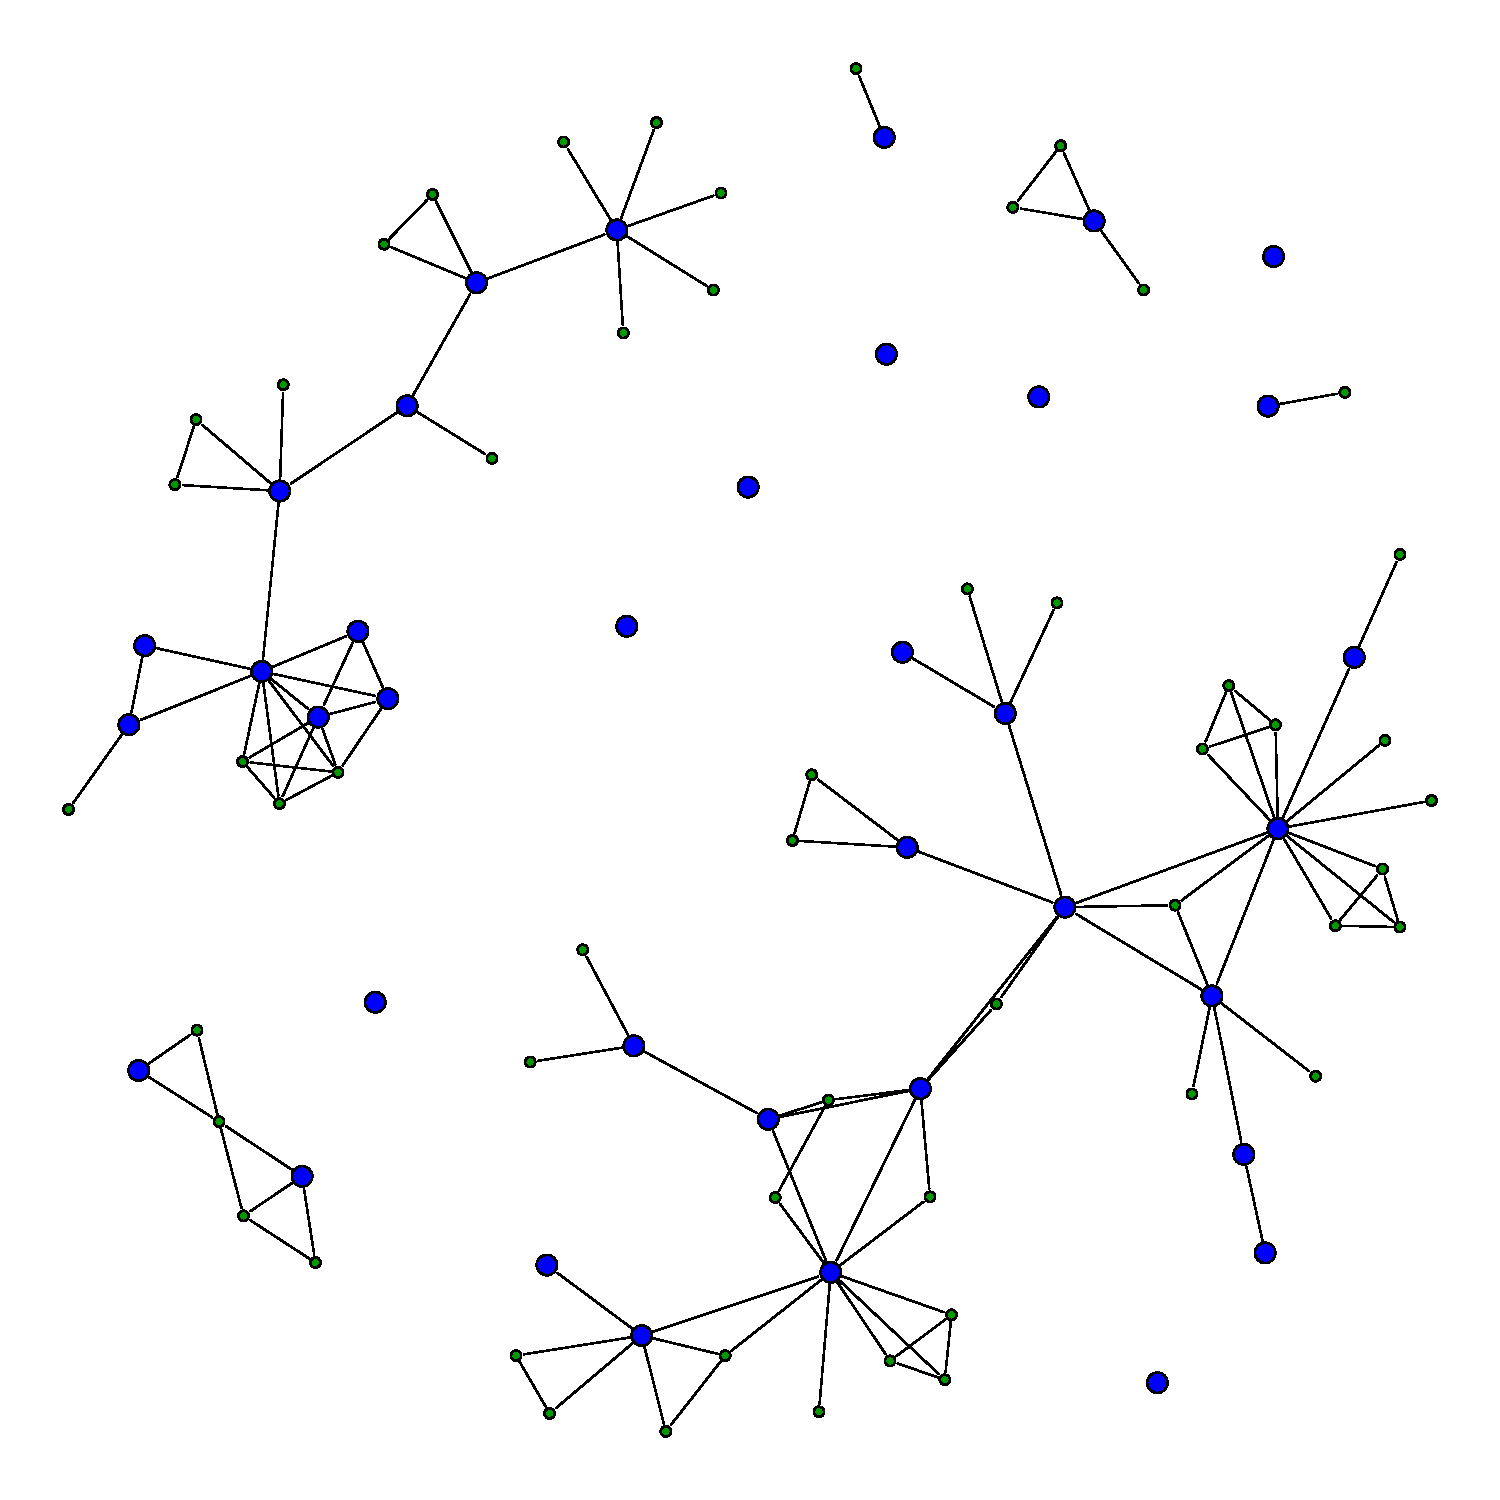
\includegraphics[width=.8\textwidth]{exemplo-grafo}
    \caption{Uma figura simples.\label{fig:subfigures:a}}
  \end{subfigure}
  % ATENÇÃO: Se você deixar uma linha em branco entre as subfiguras,
  % LaTeX vai considerar que cada uma delas pertence a um "parágrafo"
  % diferente e, portanto, vai colocá-las em linhas separadas ao invés
  % de lado a lado.
  \begin{subfigure}{0.4\textwidth}
    \centering
    \begin{turn}{90} % package rotating
      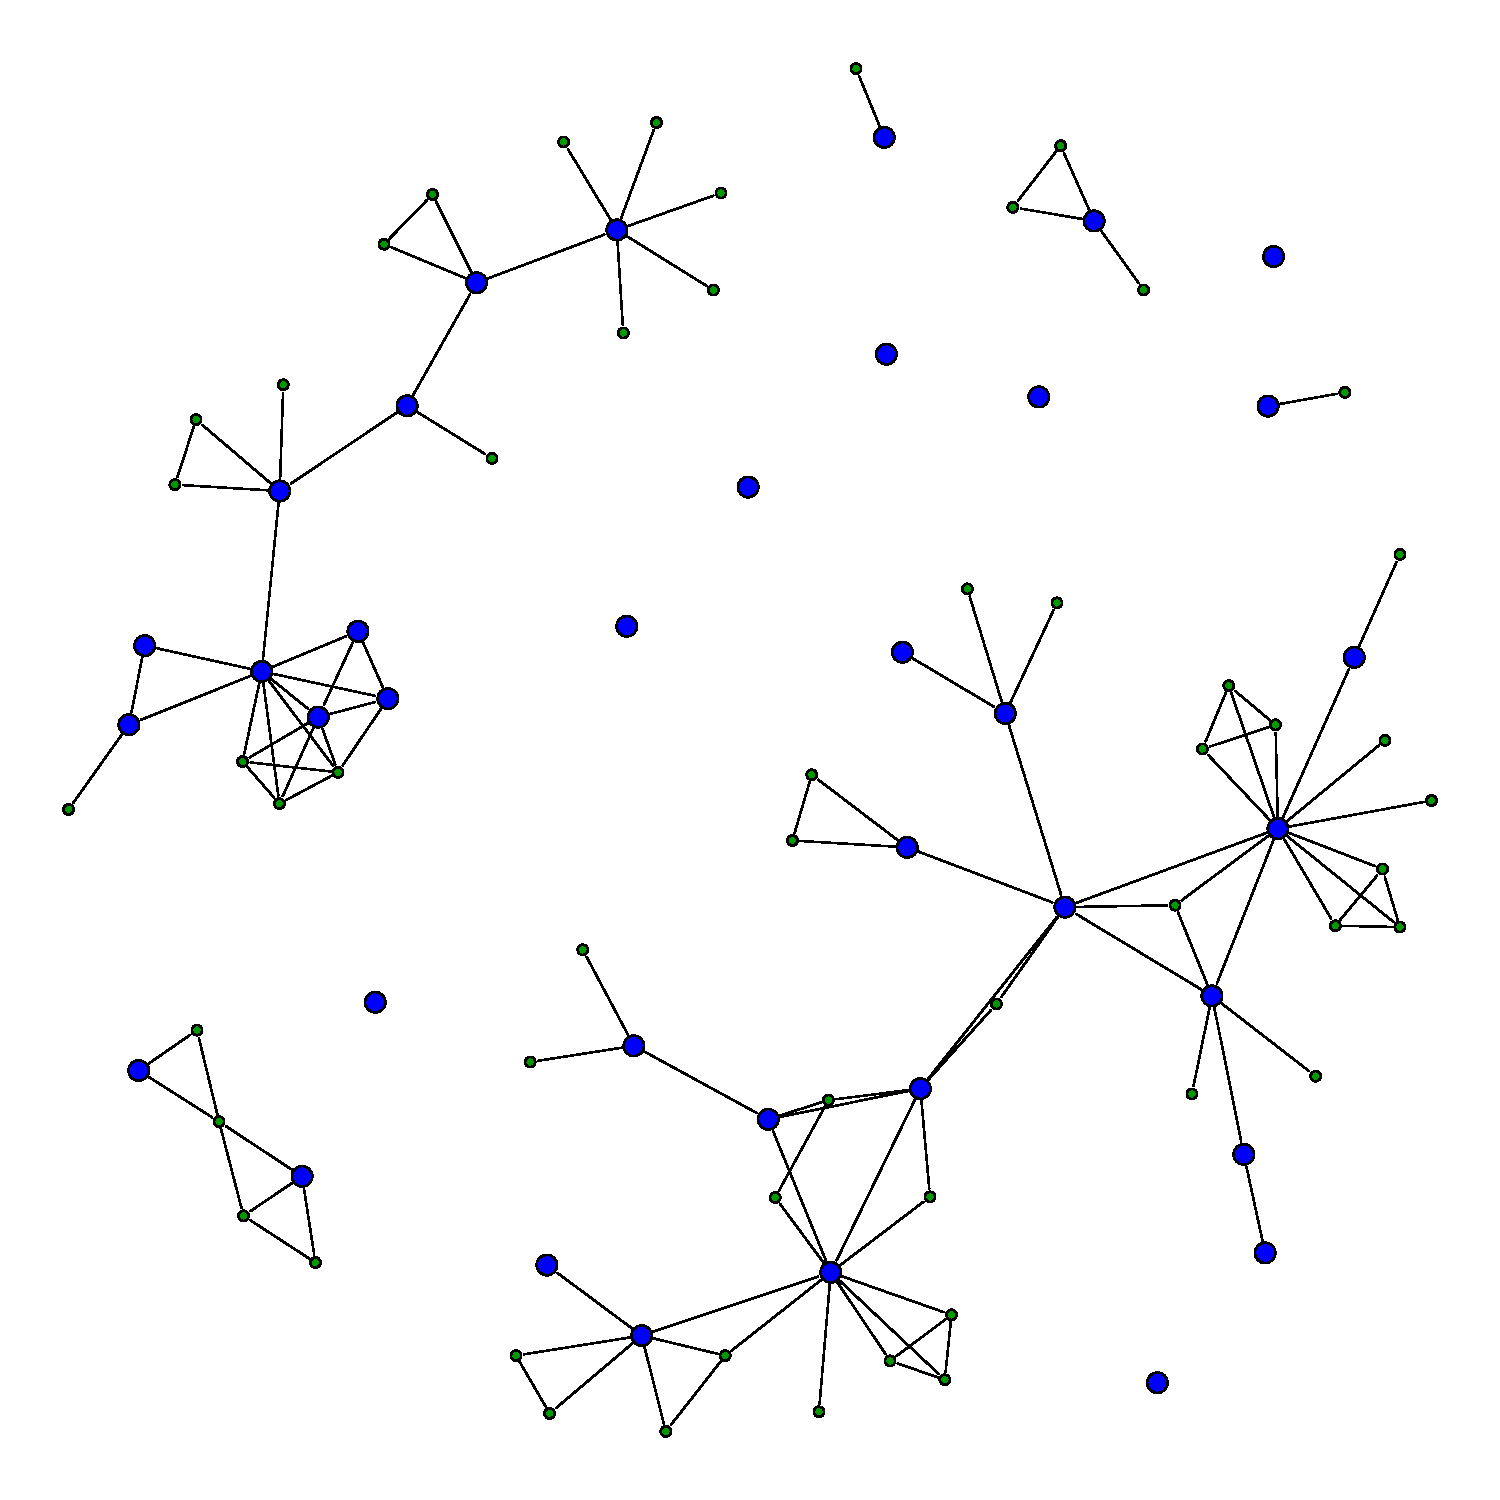
\includegraphics[width=.8\textwidth]{exemplo-grafo}
    \end{turn}
    \caption{O mesmo exemplo, girado.\label{fig:subfigures:b}}
  \end{subfigure}

  \caption{Exemplo de subfiguras.\label{fig:subfigures}}
\end{figure}

\emph{Floats} em geral incluem uma legenda e um \emph{label}.
Prefira sempre colocar o comando \textsf{\textbackslash{}label} de uma
figura ou tabela dentro do comando \textsf{\textbackslash{}caption};
não fazê-lo muitas vezes funciona, mas às vezes causa problemas.

Você pode carregar arquivos de imagem de um subdiretório usando
\texttt{dir/img.pdf}, mas é mais fácil modificar o comando
\textsf{\textbackslash{}graphicspath} próximo ao início de cada
arquivo \texttt{.tex} de exemplo.

Para centralizar uma imagem mais larga que o texto da página, use
a \emph{package} \textsf{adjustbox} (incluída neste modelo):

\begin{verbatim}
  \begin{figure}
  \adjustbox{center}{\includegraphics[width=1.2\textwidth]{img.pdf}}
  \caption{...}
  \end{figure}
\end{verbatim}

Uma ``figura'', na verdade, pode ser qualquer tipo de conteúdo ilustrativo
(um exemplo interessante é o cronograma mostrado na Figura~\ref{fig:gantt})
mas, com a \textit{package} \textsf{float}, também é possível definir ambientes
específicos para cada tipo de conteúdo adicional (cada um com numeração
independente), como é o caso do Programa~\ref{prog:java}\index{Floats}. Há
mais informações e dicas sobre recursos específicos para inclusão de
código-fonte e pseudocódigo no Apêndice \ref{ap:pseudocode}\footnote{
Observe que o nome do Apêndice (``\ref{ap:pseudocode}'') foi impresso em
uma linha separada, o que não é muito bom visualmente. Para evitar que isso
aconteça (não só no final do parágrafo, mas em qualquer quebra de linha),
utilize um espaço não-separável para fazer referências a figuras, tabelas,
seções etc. ou antes de símbolos: ``\textsf{\dots no
Apêndice\textasciitilde\textbackslash{}ref\{ap:pseudocode\}}'',
``\textsf{O discriminante é denotado
por\textasciitilde{}\$\textbackslash{}Delta\$}''.}.

%%%%%%% Cronograma %%%%%%%

\begin{figure}
  \centering

  % Package pgfgantt; veja o arquivo imegoodies.sty, em que vários
  % aspectos da aparência deste diagrama foram definidos.
  \begin{ganttchart}[
                     time slot format=isodate-yearmonth,
                     time slot unit=month,
                    ]{2017-11}{2018-5}

    \gantttitlecalendar{year,month=shortname} \ganttnewline

    \ganttgroup[progress=45]{Experimento}{2017-11}{2018-2} \ganttnewline
    \ganttbar[progress=100]{
      Preparação\ganttalignnewline
      (compra de insumos)
      }{2017-11}{2017-12} \ganttnewline
    \ganttbar[progress=30]{Execução}{2017-12}{2018-1} \ganttnewline
    \ganttbar[progress=0]{Análise}{2017-12}{2018-2} \ganttnewline

    \ganttgroup[progress=0]{Artigo}{2018-1}{2018-4} \ganttnewline
    \ganttbar[progress=0]{Escrita}{2018-1}{2018-3} \ganttnewline
    \ganttbar[progress=0]{Revisão}{2018-3}{2018-4} \ganttnewline

    \ganttmilestone{Submissão}{2018-4}
  \end{ganttchart}

  \caption{Exemplo de cronograma.\label{fig:gantt}}
\end{figure}

%%%%%%%% Código fonte %%%%%%%%

% Foi utilizado o pacote listings para formatar o código fonte.
% Veja os parâmetros de configuração no arquivo source-code.tex.
\begin{program}
  \index{Java}
  \centering

\begin{lstlisting}[language=Java, style=wider]
  for (i = 0; i < 20; i++)
  {
      // Comentário
      System.out.println("Mensagem...");
  }
\end{lstlisting}

  \caption{Exemplo de laço em Java.\label{prog:java}}
\end{program}

%%%%%

\LaTeX{} também é capaz de gerar ilustrações e diagramas diretamente, mas
usar esses recursos em geral não é trivial. Em particular, a package
\textsf{tikz} oferece bons mecanismos para a criação de figuras (incluindo
funções pré-prontas para formas geométricas, grafos, matrizes etc.) e é
fácil usá-la para traçar linhas ou curvas simples.

Gráficos de dados ou funções matemáticas de excelente qualidade podem ser
gerados com a \textit{package} \pkg{pgfplots} (há um exemplo comentado neste
arquivo; experimente des-comentar para ver o resultado). Também é possível
importar gráficos gerados por \cmd{matplotlib}, \cmd{gnuplot} e \cmd{R}
como qualquer outra imagem, mas nesse caso a fonte usada nesses gráficos
provavelmente será diferente do corpo do texto. Felizmente, isso pode ser
solucionado: \cmd{Gnuplot} (com o \emph{driver} \cmd{lua tikz}\footnote{
\url{www.gnuplot.info/docs_5.2/Gnuplot_5.2.pdf#section*.516}}),
\cmd{matplotlib} (com o \emph{backend} \textsc{pgf}\footnote{\url
{matplotlib.org/users/pgf.html}})
e \cmd{R} (com \cmd{tikzDevice}\footnote{\url
{cran.r-project.org/package=tikzDevice}}) são capazes de exportar gráficos de
dados na forma de comandos para \pkg{tikz}\footnote{Você pode se interessar
também pela \textit{package} \texttt{gnuplottex}.}: o resultado pode ser
visto na Figura~\ref{fig:graficos}.

\begin{figure}
  \centering
  \begin{subfigure}[b]{.45\textwidth}
    \input{figuras/gnuplot.tkz} % Exemplo com gnuplot
    %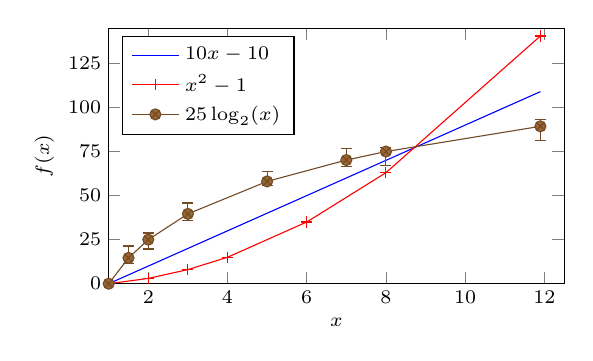
\begin{tikzpicture}
  \sffamily\scriptsize
  \begin{axis}[
    width=2.9in, height=1.9in,
    %title=Algum título,
    ylabel=$f(x)$,
    xlabel=$x$,
    xmin = 1,
    ymin = 0,
    xmax = 12.5,
    ymax = 145,
    ytick distance = 25,
    legend pos = north west,
    legend cell align = left,
  ]

  \addlegendentry{$10x-10$}
  \addplot+ [no marks] table
  {
     1.0   0
     2.0  10
     5.0  40
     7.0  60
    10.0  90
    11.9 109
  };

  \addlegendentry{$x^2-1$}
  \addplot+ [mark = +] table
  {
     1.0   0.0
     2.0   3.0
     3.0   8.0
     4.0  15.0
     6.0  35.0
     8.0  63.0
    11.9 140.6
  };
  \addlegendentry{$25\log_{2}(x)$}
  \addplot+ [error bars/y dir=both, error bars/y explicit,]
      table [y error minus index=2, y error plus index=3,]
  {
     1.0  0.00 0.0 0.0
     1.5 14.62 3.1 6.8
     2.0 25.00 5.3 3.8
     3.0 39.62 3.7 6.2
     5.0 58.05 2.2 5.5
     7.0 70.18 3.9 6.6
     8.0 75.00 7.9 2.3
    11.9 89.32 7.9 3.8
  };
  \end{axis}
\end{tikzpicture}
 % Exemplo com pgfplots
    \caption{\texttt{gnuplot}.\label{fig:gnuplot}}
  \end{subfigure}
  \begin{subfigure}[b]{.5\textwidth}
    %% Creator: Matplotlib, PGF backend
%%
%% To include the figure in your LaTeX document, write
%%   \input{<filename>.pgf}
%%
%% Make sure the required packages are loaded in your preamble
%%   \usepackage{pgf}
%%
%% and, on pdftex
%%   \usepackage[utf8]{inputenc}\DeclareUnicodeCharacter{2212}{-}
%%
%% or, on luatex and xetex
%%   \usepackage{unicode-math}
%%
%% Figures using additional raster images can only be included by \input if
%% they are in the same directory as the main LaTeX file. For loading figures
%% from other directories you can use the `import` package
%%   \usepackage{import}
%%
%% and then include the figures with
%%   \import{<path to file>}{<filename>.pgf}
%%
%% Matplotlib used the following preamble
%%   \usepackage{fontspec}
%%   \setmainfont{DejaVuSerif.ttf}[Path=/usr/share/matplotlib/mpl-data/fonts/ttf/]
%%   \setsansfont{DejaVuSans.ttf}[Path=/usr/share/matplotlib/mpl-data/fonts/ttf/]
%%   \setmonofont{DejaVuSansMono.ttf}[Path=/usr/share/matplotlib/mpl-data/fonts/ttf/]
%%
\begingroup%
\makeatletter%
\begin{pgfpicture}%
\pgfpathrectangle{\pgfpointorigin}{\pgfqpoint{2.900000in}{1.800000in}}%
\pgfusepath{use as bounding box, clip}%
\begin{pgfscope}%
\pgfsetbuttcap%
\pgfsetmiterjoin%
\definecolor{currentfill}{rgb}{1.000000,1.000000,1.000000}%
\pgfsetfillcolor{currentfill}%
\pgfsetlinewidth{0.000000pt}%
\definecolor{currentstroke}{rgb}{1.000000,1.000000,1.000000}%
\pgfsetstrokecolor{currentstroke}%
\pgfsetdash{}{0pt}%
\pgfpathmoveto{\pgfqpoint{0.000000in}{0.000000in}}%
\pgfpathlineto{\pgfqpoint{2.900000in}{0.000000in}}%
\pgfpathlineto{\pgfqpoint{2.900000in}{1.800000in}}%
\pgfpathlineto{\pgfqpoint{0.000000in}{1.800000in}}%
\pgfpathclose%
\pgfusepath{fill}%
\end{pgfscope}%
\begin{pgfscope}%
\pgfsetbuttcap%
\pgfsetmiterjoin%
\definecolor{currentfill}{rgb}{1.000000,1.000000,1.000000}%
\pgfsetfillcolor{currentfill}%
\pgfsetlinewidth{0.000000pt}%
\definecolor{currentstroke}{rgb}{0.000000,0.000000,0.000000}%
\pgfsetstrokecolor{currentstroke}%
\pgfsetstrokeopacity{0.000000}%
\pgfsetdash{}{0pt}%
\pgfpathmoveto{\pgfqpoint{0.616528in}{0.472778in}}%
\pgfpathlineto{\pgfqpoint{2.780000in}{0.472778in}}%
\pgfpathlineto{\pgfqpoint{2.780000in}{1.680000in}}%
\pgfpathlineto{\pgfqpoint{0.616528in}{1.680000in}}%
\pgfpathclose%
\pgfusepath{fill}%
\end{pgfscope}%
\begin{pgfscope}%
\pgfsetbuttcap%
\pgfsetroundjoin%
\definecolor{currentfill}{rgb}{0.000000,0.000000,0.000000}%
\pgfsetfillcolor{currentfill}%
\pgfsetlinewidth{0.803000pt}%
\definecolor{currentstroke}{rgb}{0.000000,0.000000,0.000000}%
\pgfsetstrokecolor{currentstroke}%
\pgfsetdash{}{0pt}%
\pgfsys@defobject{currentmarker}{\pgfqpoint{0.000000in}{-0.048611in}}{\pgfqpoint{0.000000in}{0.000000in}}{%
\pgfpathmoveto{\pgfqpoint{0.000000in}{0.000000in}}%
\pgfpathlineto{\pgfqpoint{0.000000in}{-0.048611in}}%
\pgfusepath{stroke,fill}%
}%
\begin{pgfscope}%
\pgfsys@transformshift{0.804656in}{0.472778in}%
\pgfsys@useobject{currentmarker}{}%
\end{pgfscope}%
\end{pgfscope}%
\begin{pgfscope}%
\definecolor{textcolor}{rgb}{0.000000,0.000000,0.000000}%
\pgfsetstrokecolor{textcolor}%
\pgfsetfillcolor{textcolor}%
\pgftext[x=0.804656in,y=0.375556in,,top]{\color{textcolor}\sffamily\fontsize{8.000000}{9.600000}\selectfont 2}%
\end{pgfscope}%
\begin{pgfscope}%
\pgfsetbuttcap%
\pgfsetroundjoin%
\definecolor{currentfill}{rgb}{0.000000,0.000000,0.000000}%
\pgfsetfillcolor{currentfill}%
\pgfsetlinewidth{0.803000pt}%
\definecolor{currentstroke}{rgb}{0.000000,0.000000,0.000000}%
\pgfsetstrokecolor{currentstroke}%
\pgfsetdash{}{0pt}%
\pgfsys@defobject{currentmarker}{\pgfqpoint{0.000000in}{-0.048611in}}{\pgfqpoint{0.000000in}{0.000000in}}{%
\pgfpathmoveto{\pgfqpoint{0.000000in}{0.000000in}}%
\pgfpathlineto{\pgfqpoint{0.000000in}{-0.048611in}}%
\pgfusepath{stroke,fill}%
}%
\begin{pgfscope}%
\pgfsys@transformshift{1.180912in}{0.472778in}%
\pgfsys@useobject{currentmarker}{}%
\end{pgfscope}%
\end{pgfscope}%
\begin{pgfscope}%
\definecolor{textcolor}{rgb}{0.000000,0.000000,0.000000}%
\pgfsetstrokecolor{textcolor}%
\pgfsetfillcolor{textcolor}%
\pgftext[x=1.180912in,y=0.375556in,,top]{\color{textcolor}\sffamily\fontsize{8.000000}{9.600000}\selectfont 4}%
\end{pgfscope}%
\begin{pgfscope}%
\pgfsetbuttcap%
\pgfsetroundjoin%
\definecolor{currentfill}{rgb}{0.000000,0.000000,0.000000}%
\pgfsetfillcolor{currentfill}%
\pgfsetlinewidth{0.803000pt}%
\definecolor{currentstroke}{rgb}{0.000000,0.000000,0.000000}%
\pgfsetstrokecolor{currentstroke}%
\pgfsetdash{}{0pt}%
\pgfsys@defobject{currentmarker}{\pgfqpoint{0.000000in}{-0.048611in}}{\pgfqpoint{0.000000in}{0.000000in}}{%
\pgfpathmoveto{\pgfqpoint{0.000000in}{0.000000in}}%
\pgfpathlineto{\pgfqpoint{0.000000in}{-0.048611in}}%
\pgfusepath{stroke,fill}%
}%
\begin{pgfscope}%
\pgfsys@transformshift{1.557168in}{0.472778in}%
\pgfsys@useobject{currentmarker}{}%
\end{pgfscope}%
\end{pgfscope}%
\begin{pgfscope}%
\definecolor{textcolor}{rgb}{0.000000,0.000000,0.000000}%
\pgfsetstrokecolor{textcolor}%
\pgfsetfillcolor{textcolor}%
\pgftext[x=1.557168in,y=0.375556in,,top]{\color{textcolor}\sffamily\fontsize{8.000000}{9.600000}\selectfont 6}%
\end{pgfscope}%
\begin{pgfscope}%
\pgfsetbuttcap%
\pgfsetroundjoin%
\definecolor{currentfill}{rgb}{0.000000,0.000000,0.000000}%
\pgfsetfillcolor{currentfill}%
\pgfsetlinewidth{0.803000pt}%
\definecolor{currentstroke}{rgb}{0.000000,0.000000,0.000000}%
\pgfsetstrokecolor{currentstroke}%
\pgfsetdash{}{0pt}%
\pgfsys@defobject{currentmarker}{\pgfqpoint{0.000000in}{-0.048611in}}{\pgfqpoint{0.000000in}{0.000000in}}{%
\pgfpathmoveto{\pgfqpoint{0.000000in}{0.000000in}}%
\pgfpathlineto{\pgfqpoint{0.000000in}{-0.048611in}}%
\pgfusepath{stroke,fill}%
}%
\begin{pgfscope}%
\pgfsys@transformshift{1.933424in}{0.472778in}%
\pgfsys@useobject{currentmarker}{}%
\end{pgfscope}%
\end{pgfscope}%
\begin{pgfscope}%
\definecolor{textcolor}{rgb}{0.000000,0.000000,0.000000}%
\pgfsetstrokecolor{textcolor}%
\pgfsetfillcolor{textcolor}%
\pgftext[x=1.933424in,y=0.375556in,,top]{\color{textcolor}\sffamily\fontsize{8.000000}{9.600000}\selectfont 8}%
\end{pgfscope}%
\begin{pgfscope}%
\pgfsetbuttcap%
\pgfsetroundjoin%
\definecolor{currentfill}{rgb}{0.000000,0.000000,0.000000}%
\pgfsetfillcolor{currentfill}%
\pgfsetlinewidth{0.803000pt}%
\definecolor{currentstroke}{rgb}{0.000000,0.000000,0.000000}%
\pgfsetstrokecolor{currentstroke}%
\pgfsetdash{}{0pt}%
\pgfsys@defobject{currentmarker}{\pgfqpoint{0.000000in}{-0.048611in}}{\pgfqpoint{0.000000in}{0.000000in}}{%
\pgfpathmoveto{\pgfqpoint{0.000000in}{0.000000in}}%
\pgfpathlineto{\pgfqpoint{0.000000in}{-0.048611in}}%
\pgfusepath{stroke,fill}%
}%
\begin{pgfscope}%
\pgfsys@transformshift{2.309680in}{0.472778in}%
\pgfsys@useobject{currentmarker}{}%
\end{pgfscope}%
\end{pgfscope}%
\begin{pgfscope}%
\definecolor{textcolor}{rgb}{0.000000,0.000000,0.000000}%
\pgfsetstrokecolor{textcolor}%
\pgfsetfillcolor{textcolor}%
\pgftext[x=2.309680in,y=0.375556in,,top]{\color{textcolor}\sffamily\fontsize{8.000000}{9.600000}\selectfont 10}%
\end{pgfscope}%
\begin{pgfscope}%
\pgfsetbuttcap%
\pgfsetroundjoin%
\definecolor{currentfill}{rgb}{0.000000,0.000000,0.000000}%
\pgfsetfillcolor{currentfill}%
\pgfsetlinewidth{0.803000pt}%
\definecolor{currentstroke}{rgb}{0.000000,0.000000,0.000000}%
\pgfsetstrokecolor{currentstroke}%
\pgfsetdash{}{0pt}%
\pgfsys@defobject{currentmarker}{\pgfqpoint{0.000000in}{-0.048611in}}{\pgfqpoint{0.000000in}{0.000000in}}{%
\pgfpathmoveto{\pgfqpoint{0.000000in}{0.000000in}}%
\pgfpathlineto{\pgfqpoint{0.000000in}{-0.048611in}}%
\pgfusepath{stroke,fill}%
}%
\begin{pgfscope}%
\pgfsys@transformshift{2.685936in}{0.472778in}%
\pgfsys@useobject{currentmarker}{}%
\end{pgfscope}%
\end{pgfscope}%
\begin{pgfscope}%
\definecolor{textcolor}{rgb}{0.000000,0.000000,0.000000}%
\pgfsetstrokecolor{textcolor}%
\pgfsetfillcolor{textcolor}%
\pgftext[x=2.685936in,y=0.375556in,,top]{\color{textcolor}\sffamily\fontsize{8.000000}{9.600000}\selectfont 12}%
\end{pgfscope}%
\begin{pgfscope}%
\definecolor{textcolor}{rgb}{0.000000,0.000000,0.000000}%
\pgfsetstrokecolor{textcolor}%
\pgfsetfillcolor{textcolor}%
\pgftext[x=1.698264in,y=0.212470in,,top]{\color{textcolor}\sffamily\fontsize{8.000000}{9.600000}\selectfont \(\displaystyle x\)}%
\end{pgfscope}%
\begin{pgfscope}%
\pgfsetbuttcap%
\pgfsetroundjoin%
\definecolor{currentfill}{rgb}{0.000000,0.000000,0.000000}%
\pgfsetfillcolor{currentfill}%
\pgfsetlinewidth{0.803000pt}%
\definecolor{currentstroke}{rgb}{0.000000,0.000000,0.000000}%
\pgfsetstrokecolor{currentstroke}%
\pgfsetdash{}{0pt}%
\pgfsys@defobject{currentmarker}{\pgfqpoint{-0.048611in}{0.000000in}}{\pgfqpoint{-0.000000in}{0.000000in}}{%
\pgfpathmoveto{\pgfqpoint{-0.000000in}{0.000000in}}%
\pgfpathlineto{\pgfqpoint{-0.048611in}{0.000000in}}%
\pgfusepath{stroke,fill}%
}%
\begin{pgfscope}%
\pgfsys@transformshift{0.616528in}{0.472778in}%
\pgfsys@useobject{currentmarker}{}%
\end{pgfscope}%
\end{pgfscope}%
\begin{pgfscope}%
\definecolor{textcolor}{rgb}{0.000000,0.000000,0.000000}%
\pgfsetstrokecolor{textcolor}%
\pgfsetfillcolor{textcolor}%
\pgftext[x=0.448613in, y=0.430569in, left, base]{\color{textcolor}\sffamily\fontsize{8.000000}{9.600000}\selectfont 0}%
\end{pgfscope}%
\begin{pgfscope}%
\pgfsetbuttcap%
\pgfsetroundjoin%
\definecolor{currentfill}{rgb}{0.000000,0.000000,0.000000}%
\pgfsetfillcolor{currentfill}%
\pgfsetlinewidth{0.803000pt}%
\definecolor{currentstroke}{rgb}{0.000000,0.000000,0.000000}%
\pgfsetstrokecolor{currentstroke}%
\pgfsetdash{}{0pt}%
\pgfsys@defobject{currentmarker}{\pgfqpoint{-0.048611in}{0.000000in}}{\pgfqpoint{-0.000000in}{0.000000in}}{%
\pgfpathmoveto{\pgfqpoint{-0.000000in}{0.000000in}}%
\pgfpathlineto{\pgfqpoint{-0.048611in}{0.000000in}}%
\pgfusepath{stroke,fill}%
}%
\begin{pgfscope}%
\pgfsys@transformshift{0.616528in}{0.680920in}%
\pgfsys@useobject{currentmarker}{}%
\end{pgfscope}%
\end{pgfscope}%
\begin{pgfscope}%
\definecolor{textcolor}{rgb}{0.000000,0.000000,0.000000}%
\pgfsetstrokecolor{textcolor}%
\pgfsetfillcolor{textcolor}%
\pgftext[x=0.377921in, y=0.638710in, left, base]{\color{textcolor}\sffamily\fontsize{8.000000}{9.600000}\selectfont 25}%
\end{pgfscope}%
\begin{pgfscope}%
\pgfsetbuttcap%
\pgfsetroundjoin%
\definecolor{currentfill}{rgb}{0.000000,0.000000,0.000000}%
\pgfsetfillcolor{currentfill}%
\pgfsetlinewidth{0.803000pt}%
\definecolor{currentstroke}{rgb}{0.000000,0.000000,0.000000}%
\pgfsetstrokecolor{currentstroke}%
\pgfsetdash{}{0pt}%
\pgfsys@defobject{currentmarker}{\pgfqpoint{-0.048611in}{0.000000in}}{\pgfqpoint{-0.000000in}{0.000000in}}{%
\pgfpathmoveto{\pgfqpoint{-0.000000in}{0.000000in}}%
\pgfpathlineto{\pgfqpoint{-0.048611in}{0.000000in}}%
\pgfusepath{stroke,fill}%
}%
\begin{pgfscope}%
\pgfsys@transformshift{0.616528in}{0.889061in}%
\pgfsys@useobject{currentmarker}{}%
\end{pgfscope}%
\end{pgfscope}%
\begin{pgfscope}%
\definecolor{textcolor}{rgb}{0.000000,0.000000,0.000000}%
\pgfsetstrokecolor{textcolor}%
\pgfsetfillcolor{textcolor}%
\pgftext[x=0.377921in, y=0.846852in, left, base]{\color{textcolor}\sffamily\fontsize{8.000000}{9.600000}\selectfont 50}%
\end{pgfscope}%
\begin{pgfscope}%
\pgfsetbuttcap%
\pgfsetroundjoin%
\definecolor{currentfill}{rgb}{0.000000,0.000000,0.000000}%
\pgfsetfillcolor{currentfill}%
\pgfsetlinewidth{0.803000pt}%
\definecolor{currentstroke}{rgb}{0.000000,0.000000,0.000000}%
\pgfsetstrokecolor{currentstroke}%
\pgfsetdash{}{0pt}%
\pgfsys@defobject{currentmarker}{\pgfqpoint{-0.048611in}{0.000000in}}{\pgfqpoint{-0.000000in}{0.000000in}}{%
\pgfpathmoveto{\pgfqpoint{-0.000000in}{0.000000in}}%
\pgfpathlineto{\pgfqpoint{-0.048611in}{0.000000in}}%
\pgfusepath{stroke,fill}%
}%
\begin{pgfscope}%
\pgfsys@transformshift{0.616528in}{1.097203in}%
\pgfsys@useobject{currentmarker}{}%
\end{pgfscope}%
\end{pgfscope}%
\begin{pgfscope}%
\definecolor{textcolor}{rgb}{0.000000,0.000000,0.000000}%
\pgfsetstrokecolor{textcolor}%
\pgfsetfillcolor{textcolor}%
\pgftext[x=0.377921in, y=1.054994in, left, base]{\color{textcolor}\sffamily\fontsize{8.000000}{9.600000}\selectfont 75}%
\end{pgfscope}%
\begin{pgfscope}%
\pgfsetbuttcap%
\pgfsetroundjoin%
\definecolor{currentfill}{rgb}{0.000000,0.000000,0.000000}%
\pgfsetfillcolor{currentfill}%
\pgfsetlinewidth{0.803000pt}%
\definecolor{currentstroke}{rgb}{0.000000,0.000000,0.000000}%
\pgfsetstrokecolor{currentstroke}%
\pgfsetdash{}{0pt}%
\pgfsys@defobject{currentmarker}{\pgfqpoint{-0.048611in}{0.000000in}}{\pgfqpoint{-0.000000in}{0.000000in}}{%
\pgfpathmoveto{\pgfqpoint{-0.000000in}{0.000000in}}%
\pgfpathlineto{\pgfqpoint{-0.048611in}{0.000000in}}%
\pgfusepath{stroke,fill}%
}%
\begin{pgfscope}%
\pgfsys@transformshift{0.616528in}{1.305345in}%
\pgfsys@useobject{currentmarker}{}%
\end{pgfscope}%
\end{pgfscope}%
\begin{pgfscope}%
\definecolor{textcolor}{rgb}{0.000000,0.000000,0.000000}%
\pgfsetstrokecolor{textcolor}%
\pgfsetfillcolor{textcolor}%
\pgftext[x=0.307229in, y=1.263136in, left, base]{\color{textcolor}\sffamily\fontsize{8.000000}{9.600000}\selectfont 100}%
\end{pgfscope}%
\begin{pgfscope}%
\pgfsetbuttcap%
\pgfsetroundjoin%
\definecolor{currentfill}{rgb}{0.000000,0.000000,0.000000}%
\pgfsetfillcolor{currentfill}%
\pgfsetlinewidth{0.803000pt}%
\definecolor{currentstroke}{rgb}{0.000000,0.000000,0.000000}%
\pgfsetstrokecolor{currentstroke}%
\pgfsetdash{}{0pt}%
\pgfsys@defobject{currentmarker}{\pgfqpoint{-0.048611in}{0.000000in}}{\pgfqpoint{-0.000000in}{0.000000in}}{%
\pgfpathmoveto{\pgfqpoint{-0.000000in}{0.000000in}}%
\pgfpathlineto{\pgfqpoint{-0.048611in}{0.000000in}}%
\pgfusepath{stroke,fill}%
}%
\begin{pgfscope}%
\pgfsys@transformshift{0.616528in}{1.513487in}%
\pgfsys@useobject{currentmarker}{}%
\end{pgfscope}%
\end{pgfscope}%
\begin{pgfscope}%
\definecolor{textcolor}{rgb}{0.000000,0.000000,0.000000}%
\pgfsetstrokecolor{textcolor}%
\pgfsetfillcolor{textcolor}%
\pgftext[x=0.307229in, y=1.471277in, left, base]{\color{textcolor}\sffamily\fontsize{8.000000}{9.600000}\selectfont 125}%
\end{pgfscope}%
\begin{pgfscope}%
\definecolor{textcolor}{rgb}{0.000000,0.000000,0.000000}%
\pgfsetstrokecolor{textcolor}%
\pgfsetfillcolor{textcolor}%
\pgftext[x=0.251673in,y=1.076389in,,bottom,rotate=90.000000]{\color{textcolor}\sffamily\fontsize{8.000000}{9.600000}\selectfont \(\displaystyle f(x)\)}%
\end{pgfscope}%
\begin{pgfscope}%
\pgfpathrectangle{\pgfqpoint{0.616528in}{0.472778in}}{\pgfqpoint{2.163472in}{1.207222in}}%
\pgfusepath{clip}%
\pgfsetbuttcap%
\pgfsetroundjoin%
\pgfsetlinewidth{0.501875pt}%
\definecolor{currentstroke}{rgb}{0.172549,0.627451,0.172549}%
\pgfsetstrokecolor{currentstroke}%
\pgfsetdash{}{0pt}%
\pgfpathmoveto{\pgfqpoint{0.616528in}{0.472778in}}%
\pgfpathlineto{\pgfqpoint{0.616528in}{0.472778in}}%
\pgfusepath{stroke}%
\end{pgfscope}%
\begin{pgfscope}%
\pgfpathrectangle{\pgfqpoint{0.616528in}{0.472778in}}{\pgfqpoint{2.163472in}{1.207222in}}%
\pgfusepath{clip}%
\pgfsetbuttcap%
\pgfsetroundjoin%
\pgfsetlinewidth{0.501875pt}%
\definecolor{currentstroke}{rgb}{0.172549,0.627451,0.172549}%
\pgfsetstrokecolor{currentstroke}%
\pgfsetdash{}{0pt}%
\pgfpathmoveto{\pgfqpoint{0.710592in}{0.568690in}}%
\pgfpathlineto{\pgfqpoint{0.710592in}{0.651114in}}%
\pgfusepath{stroke}%
\end{pgfscope}%
\begin{pgfscope}%
\pgfpathrectangle{\pgfqpoint{0.616528in}{0.472778in}}{\pgfqpoint{2.163472in}{1.207222in}}%
\pgfusepath{clip}%
\pgfsetbuttcap%
\pgfsetroundjoin%
\pgfsetlinewidth{0.501875pt}%
\definecolor{currentstroke}{rgb}{0.172549,0.627451,0.172549}%
\pgfsetstrokecolor{currentstroke}%
\pgfsetdash{}{0pt}%
\pgfpathmoveto{\pgfqpoint{0.804656in}{0.636793in}}%
\pgfpathlineto{\pgfqpoint{0.804656in}{0.712557in}}%
\pgfusepath{stroke}%
\end{pgfscope}%
\begin{pgfscope}%
\pgfpathrectangle{\pgfqpoint{0.616528in}{0.472778in}}{\pgfqpoint{2.163472in}{1.207222in}}%
\pgfusepath{clip}%
\pgfsetbuttcap%
\pgfsetroundjoin%
\pgfsetlinewidth{0.501875pt}%
\definecolor{currentstroke}{rgb}{0.172549,0.627451,0.172549}%
\pgfsetstrokecolor{currentstroke}%
\pgfsetdash{}{0pt}%
\pgfpathmoveto{\pgfqpoint{0.992784in}{0.771836in}}%
\pgfpathlineto{\pgfqpoint{0.992784in}{0.854260in}}%
\pgfusepath{stroke}%
\end{pgfscope}%
\begin{pgfscope}%
\pgfpathrectangle{\pgfqpoint{0.616528in}{0.472778in}}{\pgfqpoint{2.163472in}{1.207222in}}%
\pgfusepath{clip}%
\pgfsetbuttcap%
\pgfsetroundjoin%
\pgfsetlinewidth{0.501875pt}%
\definecolor{currentstroke}{rgb}{0.172549,0.627451,0.172549}%
\pgfsetstrokecolor{currentstroke}%
\pgfsetdash{}{0pt}%
\pgfpathmoveto{\pgfqpoint{1.369040in}{0.937766in}}%
\pgfpathlineto{\pgfqpoint{1.369040in}{1.001874in}}%
\pgfusepath{stroke}%
\end{pgfscope}%
\begin{pgfscope}%
\pgfpathrectangle{\pgfqpoint{0.616528in}{0.472778in}}{\pgfqpoint{2.163472in}{1.207222in}}%
\pgfusepath{clip}%
\pgfsetbuttcap%
\pgfsetroundjoin%
\pgfsetlinewidth{0.501875pt}%
\definecolor{currentstroke}{rgb}{0.172549,0.627451,0.172549}%
\pgfsetstrokecolor{currentstroke}%
\pgfsetdash{}{0pt}%
\pgfpathmoveto{\pgfqpoint{1.745296in}{1.024603in}}%
\pgfpathlineto{\pgfqpoint{1.745296in}{1.112023in}}%
\pgfusepath{stroke}%
\end{pgfscope}%
\begin{pgfscope}%
\pgfpathrectangle{\pgfqpoint{0.616528in}{0.472778in}}{\pgfqpoint{2.163472in}{1.207222in}}%
\pgfusepath{clip}%
\pgfsetbuttcap%
\pgfsetroundjoin%
\pgfsetlinewidth{0.501875pt}%
\definecolor{currentstroke}{rgb}{0.172549,0.627451,0.172549}%
\pgfsetstrokecolor{currentstroke}%
\pgfsetdash{}{0pt}%
\pgfpathmoveto{\pgfqpoint{1.933424in}{1.031430in}}%
\pgfpathlineto{\pgfqpoint{1.933424in}{1.116352in}}%
\pgfusepath{stroke}%
\end{pgfscope}%
\begin{pgfscope}%
\pgfpathrectangle{\pgfqpoint{0.616528in}{0.472778in}}{\pgfqpoint{2.163472in}{1.207222in}}%
\pgfusepath{clip}%
\pgfsetbuttcap%
\pgfsetroundjoin%
\pgfsetlinewidth{0.501875pt}%
\definecolor{currentstroke}{rgb}{0.172549,0.627451,0.172549}%
\pgfsetstrokecolor{currentstroke}%
\pgfsetdash{}{0pt}%
\pgfpathmoveto{\pgfqpoint{2.667123in}{1.150654in}}%
\pgfpathlineto{\pgfqpoint{2.667123in}{1.248064in}}%
\pgfusepath{stroke}%
\end{pgfscope}%
\begin{pgfscope}%
\pgfpathrectangle{\pgfqpoint{0.616528in}{0.472778in}}{\pgfqpoint{2.163472in}{1.207222in}}%
\pgfusepath{clip}%
\pgfsetrectcap%
\pgfsetroundjoin%
\pgfsetlinewidth{1.003750pt}%
\definecolor{currentstroke}{rgb}{0.121569,0.466667,0.705882}%
\pgfsetstrokecolor{currentstroke}%
\pgfsetdash{}{0pt}%
\pgfpathmoveto{\pgfqpoint{0.616528in}{0.472778in}}%
\pgfpathlineto{\pgfqpoint{0.635341in}{0.481103in}}%
\pgfpathlineto{\pgfqpoint{0.654153in}{0.489429in}}%
\pgfpathlineto{\pgfqpoint{0.672966in}{0.497755in}}%
\pgfpathlineto{\pgfqpoint{0.691779in}{0.506080in}}%
\pgfpathlineto{\pgfqpoint{0.710592in}{0.514406in}}%
\pgfpathlineto{\pgfqpoint{0.729405in}{0.522732in}}%
\pgfpathlineto{\pgfqpoint{0.748217in}{0.531057in}}%
\pgfpathlineto{\pgfqpoint{0.767030in}{0.539383in}}%
\pgfpathlineto{\pgfqpoint{0.785843in}{0.547709in}}%
\pgfpathlineto{\pgfqpoint{0.804656in}{0.556034in}}%
\pgfpathlineto{\pgfqpoint{0.823469in}{0.564360in}}%
\pgfpathlineto{\pgfqpoint{0.842281in}{0.572686in}}%
\pgfpathlineto{\pgfqpoint{0.861094in}{0.581011in}}%
\pgfpathlineto{\pgfqpoint{0.879907in}{0.589337in}}%
\pgfpathlineto{\pgfqpoint{0.898720in}{0.597663in}}%
\pgfpathlineto{\pgfqpoint{0.917533in}{0.605989in}}%
\pgfpathlineto{\pgfqpoint{0.936345in}{0.614314in}}%
\pgfpathlineto{\pgfqpoint{0.955158in}{0.622640in}}%
\pgfpathlineto{\pgfqpoint{0.973971in}{0.630966in}}%
\pgfpathlineto{\pgfqpoint{0.992784in}{0.639291in}}%
\pgfpathlineto{\pgfqpoint{1.011597in}{0.647617in}}%
\pgfpathlineto{\pgfqpoint{1.030409in}{0.655943in}}%
\pgfpathlineto{\pgfqpoint{1.049222in}{0.664268in}}%
\pgfpathlineto{\pgfqpoint{1.068035in}{0.672594in}}%
\pgfpathlineto{\pgfqpoint{1.086848in}{0.680920in}}%
\pgfpathlineto{\pgfqpoint{1.105661in}{0.689245in}}%
\pgfpathlineto{\pgfqpoint{1.124473in}{0.697571in}}%
\pgfpathlineto{\pgfqpoint{1.143286in}{0.705897in}}%
\pgfpathlineto{\pgfqpoint{1.162099in}{0.714222in}}%
\pgfpathlineto{\pgfqpoint{1.180912in}{0.722548in}}%
\pgfpathlineto{\pgfqpoint{1.199725in}{0.730874in}}%
\pgfpathlineto{\pgfqpoint{1.218537in}{0.739199in}}%
\pgfpathlineto{\pgfqpoint{1.237350in}{0.747525in}}%
\pgfpathlineto{\pgfqpoint{1.256163in}{0.755851in}}%
\pgfpathlineto{\pgfqpoint{1.274976in}{0.764176in}}%
\pgfpathlineto{\pgfqpoint{1.293789in}{0.772502in}}%
\pgfpathlineto{\pgfqpoint{1.312601in}{0.780828in}}%
\pgfpathlineto{\pgfqpoint{1.331414in}{0.789153in}}%
\pgfpathlineto{\pgfqpoint{1.350227in}{0.797479in}}%
\pgfpathlineto{\pgfqpoint{1.369040in}{0.805805in}}%
\pgfpathlineto{\pgfqpoint{1.387853in}{0.814130in}}%
\pgfpathlineto{\pgfqpoint{1.406665in}{0.822456in}}%
\pgfpathlineto{\pgfqpoint{1.425478in}{0.830782in}}%
\pgfpathlineto{\pgfqpoint{1.444291in}{0.839107in}}%
\pgfpathlineto{\pgfqpoint{1.463104in}{0.847433in}}%
\pgfpathlineto{\pgfqpoint{1.481917in}{0.855759in}}%
\pgfpathlineto{\pgfqpoint{1.500729in}{0.864084in}}%
\pgfpathlineto{\pgfqpoint{1.519542in}{0.872410in}}%
\pgfpathlineto{\pgfqpoint{1.538355in}{0.880736in}}%
\pgfpathlineto{\pgfqpoint{1.557168in}{0.889061in}}%
\pgfpathlineto{\pgfqpoint{1.575981in}{0.897387in}}%
\pgfpathlineto{\pgfqpoint{1.594793in}{0.905713in}}%
\pgfpathlineto{\pgfqpoint{1.613606in}{0.914038in}}%
\pgfpathlineto{\pgfqpoint{1.632419in}{0.922364in}}%
\pgfpathlineto{\pgfqpoint{1.651232in}{0.930690in}}%
\pgfpathlineto{\pgfqpoint{1.670045in}{0.939015in}}%
\pgfpathlineto{\pgfqpoint{1.688857in}{0.947341in}}%
\pgfpathlineto{\pgfqpoint{1.707670in}{0.955667in}}%
\pgfpathlineto{\pgfqpoint{1.726483in}{0.963992in}}%
\pgfpathlineto{\pgfqpoint{1.745296in}{0.972318in}}%
\pgfpathlineto{\pgfqpoint{1.764109in}{0.980644in}}%
\pgfpathlineto{\pgfqpoint{1.782921in}{0.988969in}}%
\pgfpathlineto{\pgfqpoint{1.801734in}{0.997295in}}%
\pgfpathlineto{\pgfqpoint{1.820547in}{1.005621in}}%
\pgfpathlineto{\pgfqpoint{1.839360in}{1.013946in}}%
\pgfpathlineto{\pgfqpoint{1.858173in}{1.022272in}}%
\pgfpathlineto{\pgfqpoint{1.876986in}{1.030598in}}%
\pgfpathlineto{\pgfqpoint{1.895798in}{1.038923in}}%
\pgfpathlineto{\pgfqpoint{1.914611in}{1.047249in}}%
\pgfpathlineto{\pgfqpoint{1.933424in}{1.055575in}}%
\pgfpathlineto{\pgfqpoint{1.952237in}{1.063900in}}%
\pgfpathlineto{\pgfqpoint{1.971050in}{1.072226in}}%
\pgfpathlineto{\pgfqpoint{1.989862in}{1.080552in}}%
\pgfpathlineto{\pgfqpoint{2.008675in}{1.088877in}}%
\pgfpathlineto{\pgfqpoint{2.027488in}{1.097203in}}%
\pgfpathlineto{\pgfqpoint{2.046301in}{1.105529in}}%
\pgfpathlineto{\pgfqpoint{2.065114in}{1.113854in}}%
\pgfpathlineto{\pgfqpoint{2.083926in}{1.122180in}}%
\pgfpathlineto{\pgfqpoint{2.102739in}{1.130506in}}%
\pgfpathlineto{\pgfqpoint{2.121552in}{1.138831in}}%
\pgfpathlineto{\pgfqpoint{2.140365in}{1.147157in}}%
\pgfpathlineto{\pgfqpoint{2.159178in}{1.155483in}}%
\pgfpathlineto{\pgfqpoint{2.177990in}{1.163808in}}%
\pgfpathlineto{\pgfqpoint{2.196803in}{1.172134in}}%
\pgfpathlineto{\pgfqpoint{2.215616in}{1.180460in}}%
\pgfpathlineto{\pgfqpoint{2.234429in}{1.188785in}}%
\pgfpathlineto{\pgfqpoint{2.253242in}{1.197111in}}%
\pgfpathlineto{\pgfqpoint{2.272054in}{1.205437in}}%
\pgfpathlineto{\pgfqpoint{2.290867in}{1.213762in}}%
\pgfpathlineto{\pgfqpoint{2.309680in}{1.222088in}}%
\pgfpathlineto{\pgfqpoint{2.328493in}{1.230414in}}%
\pgfpathlineto{\pgfqpoint{2.347306in}{1.238739in}}%
\pgfpathlineto{\pgfqpoint{2.366118in}{1.247065in}}%
\pgfpathlineto{\pgfqpoint{2.384931in}{1.255391in}}%
\pgfpathlineto{\pgfqpoint{2.403744in}{1.263716in}}%
\pgfpathlineto{\pgfqpoint{2.422557in}{1.272042in}}%
\pgfpathlineto{\pgfqpoint{2.441370in}{1.280368in}}%
\pgfpathlineto{\pgfqpoint{2.460182in}{1.288693in}}%
\pgfpathlineto{\pgfqpoint{2.478995in}{1.297019in}}%
\pgfpathlineto{\pgfqpoint{2.497808in}{1.305345in}}%
\pgfpathlineto{\pgfqpoint{2.516621in}{1.313670in}}%
\pgfpathlineto{\pgfqpoint{2.535434in}{1.321996in}}%
\pgfpathlineto{\pgfqpoint{2.554246in}{1.330322in}}%
\pgfpathlineto{\pgfqpoint{2.573059in}{1.338648in}}%
\pgfpathlineto{\pgfqpoint{2.591872in}{1.346973in}}%
\pgfpathlineto{\pgfqpoint{2.610685in}{1.355299in}}%
\pgfpathlineto{\pgfqpoint{2.629498in}{1.363625in}}%
\pgfpathlineto{\pgfqpoint{2.648310in}{1.371950in}}%
\pgfpathlineto{\pgfqpoint{2.667123in}{1.380276in}}%
\pgfusepath{stroke}%
\end{pgfscope}%
\begin{pgfscope}%
\pgfpathrectangle{\pgfqpoint{0.616528in}{0.472778in}}{\pgfqpoint{2.163472in}{1.207222in}}%
\pgfusepath{clip}%
\pgfsetrectcap%
\pgfsetroundjoin%
\pgfsetlinewidth{1.003750pt}%
\definecolor{currentstroke}{rgb}{1.000000,0.498039,0.054902}%
\pgfsetstrokecolor{currentstroke}%
\pgfsetdash{}{0pt}%
\pgfpathmoveto{\pgfqpoint{0.616528in}{0.472778in}}%
\pgfpathlineto{\pgfqpoint{0.804656in}{0.497755in}}%
\pgfpathlineto{\pgfqpoint{0.992784in}{0.539383in}}%
\pgfpathlineto{\pgfqpoint{1.180912in}{0.597663in}}%
\pgfpathlineto{\pgfqpoint{1.557168in}{0.764176in}}%
\pgfpathlineto{\pgfqpoint{1.933424in}{0.997295in}}%
\pgfpathlineto{\pgfqpoint{2.667123in}{1.643450in}}%
\pgfusepath{stroke}%
\end{pgfscope}%
\begin{pgfscope}%
\pgfpathrectangle{\pgfqpoint{0.616528in}{0.472778in}}{\pgfqpoint{2.163472in}{1.207222in}}%
\pgfusepath{clip}%
\pgfsetbuttcap%
\pgfsetroundjoin%
\definecolor{currentfill}{rgb}{1.000000,0.498039,0.054902}%
\pgfsetfillcolor{currentfill}%
\pgfsetlinewidth{1.003750pt}%
\definecolor{currentstroke}{rgb}{1.000000,0.498039,0.054902}%
\pgfsetstrokecolor{currentstroke}%
\pgfsetdash{}{0pt}%
\pgfsys@defobject{currentmarker}{\pgfqpoint{-0.034722in}{-0.034722in}}{\pgfqpoint{0.034722in}{0.034722in}}{%
\pgfpathmoveto{\pgfqpoint{-0.034722in}{0.000000in}}%
\pgfpathlineto{\pgfqpoint{0.034722in}{0.000000in}}%
\pgfpathmoveto{\pgfqpoint{0.000000in}{-0.034722in}}%
\pgfpathlineto{\pgfqpoint{0.000000in}{0.034722in}}%
\pgfusepath{stroke,fill}%
}%
\begin{pgfscope}%
\pgfsys@transformshift{0.616528in}{0.472778in}%
\pgfsys@useobject{currentmarker}{}%
\end{pgfscope}%
\begin{pgfscope}%
\pgfsys@transformshift{0.804656in}{0.497755in}%
\pgfsys@useobject{currentmarker}{}%
\end{pgfscope}%
\begin{pgfscope}%
\pgfsys@transformshift{0.992784in}{0.539383in}%
\pgfsys@useobject{currentmarker}{}%
\end{pgfscope}%
\begin{pgfscope}%
\pgfsys@transformshift{1.180912in}{0.597663in}%
\pgfsys@useobject{currentmarker}{}%
\end{pgfscope}%
\begin{pgfscope}%
\pgfsys@transformshift{1.557168in}{0.764176in}%
\pgfsys@useobject{currentmarker}{}%
\end{pgfscope}%
\begin{pgfscope}%
\pgfsys@transformshift{1.933424in}{0.997295in}%
\pgfsys@useobject{currentmarker}{}%
\end{pgfscope}%
\begin{pgfscope}%
\pgfsys@transformshift{2.667123in}{1.643450in}%
\pgfsys@useobject{currentmarker}{}%
\end{pgfscope}%
\end{pgfscope}%
\begin{pgfscope}%
\pgfpathrectangle{\pgfqpoint{0.616528in}{0.472778in}}{\pgfqpoint{2.163472in}{1.207222in}}%
\pgfusepath{clip}%
\pgfsetbuttcap%
\pgfsetroundjoin%
\definecolor{currentfill}{rgb}{0.172549,0.627451,0.172549}%
\pgfsetfillcolor{currentfill}%
\pgfsetlinewidth{0.501875pt}%
\definecolor{currentstroke}{rgb}{0.172549,0.627451,0.172549}%
\pgfsetstrokecolor{currentstroke}%
\pgfsetdash{}{0pt}%
\pgfsys@defobject{currentmarker}{\pgfqpoint{-0.027778in}{-0.000000in}}{\pgfqpoint{0.027778in}{0.000000in}}{%
\pgfpathmoveto{\pgfqpoint{0.027778in}{-0.000000in}}%
\pgfpathlineto{\pgfqpoint{-0.027778in}{0.000000in}}%
\pgfusepath{stroke,fill}%
}%
\begin{pgfscope}%
\pgfsys@transformshift{0.616528in}{0.472778in}%
\pgfsys@useobject{currentmarker}{}%
\end{pgfscope}%
\begin{pgfscope}%
\pgfsys@transformshift{0.710592in}{0.568690in}%
\pgfsys@useobject{currentmarker}{}%
\end{pgfscope}%
\begin{pgfscope}%
\pgfsys@transformshift{0.804656in}{0.636793in}%
\pgfsys@useobject{currentmarker}{}%
\end{pgfscope}%
\begin{pgfscope}%
\pgfsys@transformshift{0.992784in}{0.771836in}%
\pgfsys@useobject{currentmarker}{}%
\end{pgfscope}%
\begin{pgfscope}%
\pgfsys@transformshift{1.369040in}{0.937766in}%
\pgfsys@useobject{currentmarker}{}%
\end{pgfscope}%
\begin{pgfscope}%
\pgfsys@transformshift{1.745296in}{1.024603in}%
\pgfsys@useobject{currentmarker}{}%
\end{pgfscope}%
\begin{pgfscope}%
\pgfsys@transformshift{1.933424in}{1.031430in}%
\pgfsys@useobject{currentmarker}{}%
\end{pgfscope}%
\begin{pgfscope}%
\pgfsys@transformshift{2.667123in}{1.150654in}%
\pgfsys@useobject{currentmarker}{}%
\end{pgfscope}%
\end{pgfscope}%
\begin{pgfscope}%
\pgfpathrectangle{\pgfqpoint{0.616528in}{0.472778in}}{\pgfqpoint{2.163472in}{1.207222in}}%
\pgfusepath{clip}%
\pgfsetbuttcap%
\pgfsetroundjoin%
\definecolor{currentfill}{rgb}{0.172549,0.627451,0.172549}%
\pgfsetfillcolor{currentfill}%
\pgfsetlinewidth{0.501875pt}%
\definecolor{currentstroke}{rgb}{0.172549,0.627451,0.172549}%
\pgfsetstrokecolor{currentstroke}%
\pgfsetdash{}{0pt}%
\pgfsys@defobject{currentmarker}{\pgfqpoint{-0.027778in}{-0.000000in}}{\pgfqpoint{0.027778in}{0.000000in}}{%
\pgfpathmoveto{\pgfqpoint{0.027778in}{-0.000000in}}%
\pgfpathlineto{\pgfqpoint{-0.027778in}{0.000000in}}%
\pgfusepath{stroke,fill}%
}%
\begin{pgfscope}%
\pgfsys@transformshift{0.616528in}{0.472778in}%
\pgfsys@useobject{currentmarker}{}%
\end{pgfscope}%
\begin{pgfscope}%
\pgfsys@transformshift{0.710592in}{0.651114in}%
\pgfsys@useobject{currentmarker}{}%
\end{pgfscope}%
\begin{pgfscope}%
\pgfsys@transformshift{0.804656in}{0.712557in}%
\pgfsys@useobject{currentmarker}{}%
\end{pgfscope}%
\begin{pgfscope}%
\pgfsys@transformshift{0.992784in}{0.854260in}%
\pgfsys@useobject{currentmarker}{}%
\end{pgfscope}%
\begin{pgfscope}%
\pgfsys@transformshift{1.369040in}{1.001874in}%
\pgfsys@useobject{currentmarker}{}%
\end{pgfscope}%
\begin{pgfscope}%
\pgfsys@transformshift{1.745296in}{1.112023in}%
\pgfsys@useobject{currentmarker}{}%
\end{pgfscope}%
\begin{pgfscope}%
\pgfsys@transformshift{1.933424in}{1.116352in}%
\pgfsys@useobject{currentmarker}{}%
\end{pgfscope}%
\begin{pgfscope}%
\pgfsys@transformshift{2.667123in}{1.248064in}%
\pgfsys@useobject{currentmarker}{}%
\end{pgfscope}%
\end{pgfscope}%
\begin{pgfscope}%
\pgfpathrectangle{\pgfqpoint{0.616528in}{0.472778in}}{\pgfqpoint{2.163472in}{1.207222in}}%
\pgfusepath{clip}%
\pgfsetrectcap%
\pgfsetroundjoin%
\pgfsetlinewidth{1.003750pt}%
\definecolor{currentstroke}{rgb}{0.172549,0.627451,0.172549}%
\pgfsetstrokecolor{currentstroke}%
\pgfsetdash{}{0pt}%
\pgfpathmoveto{\pgfqpoint{0.616528in}{0.472778in}}%
\pgfpathlineto{\pgfqpoint{0.710592in}{0.594499in}}%
\pgfpathlineto{\pgfqpoint{0.804656in}{0.680920in}}%
\pgfpathlineto{\pgfqpoint{0.992784in}{0.802641in}}%
\pgfpathlineto{\pgfqpoint{1.369040in}{0.956083in}}%
\pgfpathlineto{\pgfqpoint{1.745296in}{1.057073in}}%
\pgfpathlineto{\pgfqpoint{1.933424in}{1.097203in}}%
\pgfpathlineto{\pgfqpoint{2.667123in}{1.216427in}}%
\pgfusepath{stroke}%
\end{pgfscope}%
\begin{pgfscope}%
\pgfpathrectangle{\pgfqpoint{0.616528in}{0.472778in}}{\pgfqpoint{2.163472in}{1.207222in}}%
\pgfusepath{clip}%
\pgfsetbuttcap%
\pgfsetroundjoin%
\definecolor{currentfill}{rgb}{0.172549,0.627451,0.172549}%
\pgfsetfillcolor{currentfill}%
\pgfsetlinewidth{0.501875pt}%
\definecolor{currentstroke}{rgb}{0.172549,0.627451,0.172549}%
\pgfsetstrokecolor{currentstroke}%
\pgfsetdash{}{0pt}%
\pgfsys@defobject{currentmarker}{\pgfqpoint{-0.017361in}{-0.017361in}}{\pgfqpoint{0.017361in}{0.017361in}}{%
\pgfpathmoveto{\pgfqpoint{0.000000in}{-0.017361in}}%
\pgfpathcurveto{\pgfqpoint{0.004604in}{-0.017361in}}{\pgfqpoint{0.009020in}{-0.015532in}}{\pgfqpoint{0.012276in}{-0.012276in}}%
\pgfpathcurveto{\pgfqpoint{0.015532in}{-0.009020in}}{\pgfqpoint{0.017361in}{-0.004604in}}{\pgfqpoint{0.017361in}{0.000000in}}%
\pgfpathcurveto{\pgfqpoint{0.017361in}{0.004604in}}{\pgfqpoint{0.015532in}{0.009020in}}{\pgfqpoint{0.012276in}{0.012276in}}%
\pgfpathcurveto{\pgfqpoint{0.009020in}{0.015532in}}{\pgfqpoint{0.004604in}{0.017361in}}{\pgfqpoint{0.000000in}{0.017361in}}%
\pgfpathcurveto{\pgfqpoint{-0.004604in}{0.017361in}}{\pgfqpoint{-0.009020in}{0.015532in}}{\pgfqpoint{-0.012276in}{0.012276in}}%
\pgfpathcurveto{\pgfqpoint{-0.015532in}{0.009020in}}{\pgfqpoint{-0.017361in}{0.004604in}}{\pgfqpoint{-0.017361in}{0.000000in}}%
\pgfpathcurveto{\pgfqpoint{-0.017361in}{-0.004604in}}{\pgfqpoint{-0.015532in}{-0.009020in}}{\pgfqpoint{-0.012276in}{-0.012276in}}%
\pgfpathcurveto{\pgfqpoint{-0.009020in}{-0.015532in}}{\pgfqpoint{-0.004604in}{-0.017361in}}{\pgfqpoint{0.000000in}{-0.017361in}}%
\pgfpathclose%
\pgfusepath{stroke,fill}%
}%
\begin{pgfscope}%
\pgfsys@transformshift{0.616528in}{0.472778in}%
\pgfsys@useobject{currentmarker}{}%
\end{pgfscope}%
\begin{pgfscope}%
\pgfsys@transformshift{0.710592in}{0.594499in}%
\pgfsys@useobject{currentmarker}{}%
\end{pgfscope}%
\begin{pgfscope}%
\pgfsys@transformshift{0.804656in}{0.680920in}%
\pgfsys@useobject{currentmarker}{}%
\end{pgfscope}%
\begin{pgfscope}%
\pgfsys@transformshift{0.992784in}{0.802641in}%
\pgfsys@useobject{currentmarker}{}%
\end{pgfscope}%
\begin{pgfscope}%
\pgfsys@transformshift{1.369040in}{0.956083in}%
\pgfsys@useobject{currentmarker}{}%
\end{pgfscope}%
\begin{pgfscope}%
\pgfsys@transformshift{1.745296in}{1.057073in}%
\pgfsys@useobject{currentmarker}{}%
\end{pgfscope}%
\begin{pgfscope}%
\pgfsys@transformshift{1.933424in}{1.097203in}%
\pgfsys@useobject{currentmarker}{}%
\end{pgfscope}%
\begin{pgfscope}%
\pgfsys@transformshift{2.667123in}{1.216427in}%
\pgfsys@useobject{currentmarker}{}%
\end{pgfscope}%
\end{pgfscope}%
\begin{pgfscope}%
\pgfsetrectcap%
\pgfsetmiterjoin%
\pgfsetlinewidth{0.803000pt}%
\definecolor{currentstroke}{rgb}{0.000000,0.000000,0.000000}%
\pgfsetstrokecolor{currentstroke}%
\pgfsetdash{}{0pt}%
\pgfpathmoveto{\pgfqpoint{0.616528in}{0.472778in}}%
\pgfpathlineto{\pgfqpoint{0.616528in}{1.680000in}}%
\pgfusepath{stroke}%
\end{pgfscope}%
\begin{pgfscope}%
\pgfsetrectcap%
\pgfsetmiterjoin%
\pgfsetlinewidth{0.803000pt}%
\definecolor{currentstroke}{rgb}{0.000000,0.000000,0.000000}%
\pgfsetstrokecolor{currentstroke}%
\pgfsetdash{}{0pt}%
\pgfpathmoveto{\pgfqpoint{2.780000in}{0.472778in}}%
\pgfpathlineto{\pgfqpoint{2.780000in}{1.680000in}}%
\pgfusepath{stroke}%
\end{pgfscope}%
\begin{pgfscope}%
\pgfsetrectcap%
\pgfsetmiterjoin%
\pgfsetlinewidth{0.803000pt}%
\definecolor{currentstroke}{rgb}{0.000000,0.000000,0.000000}%
\pgfsetstrokecolor{currentstroke}%
\pgfsetdash{}{0pt}%
\pgfpathmoveto{\pgfqpoint{0.616528in}{0.472778in}}%
\pgfpathlineto{\pgfqpoint{2.780000in}{0.472778in}}%
\pgfusepath{stroke}%
\end{pgfscope}%
\begin{pgfscope}%
\pgfsetrectcap%
\pgfsetmiterjoin%
\pgfsetlinewidth{0.803000pt}%
\definecolor{currentstroke}{rgb}{0.000000,0.000000,0.000000}%
\pgfsetstrokecolor{currentstroke}%
\pgfsetdash{}{0pt}%
\pgfpathmoveto{\pgfqpoint{0.616528in}{1.680000in}}%
\pgfpathlineto{\pgfqpoint{2.780000in}{1.680000in}}%
\pgfusepath{stroke}%
\end{pgfscope}%
\begin{pgfscope}%
\pgfsetbuttcap%
\pgfsetmiterjoin%
\definecolor{currentfill}{rgb}{1.000000,1.000000,1.000000}%
\pgfsetfillcolor{currentfill}%
\pgfsetfillopacity{0.800000}%
\pgfsetlinewidth{1.003750pt}%
\definecolor{currentstroke}{rgb}{0.800000,0.800000,0.800000}%
\pgfsetstrokecolor{currentstroke}%
\pgfsetstrokeopacity{0.800000}%
\pgfsetdash{}{0pt}%
\pgfpathmoveto{\pgfqpoint{0.694306in}{1.089431in}}%
\pgfpathlineto{\pgfqpoint{1.577299in}{1.089431in}}%
\pgfpathquadraticcurveto{\pgfqpoint{1.599521in}{1.089431in}}{\pgfqpoint{1.599521in}{1.111653in}}%
\pgfpathlineto{\pgfqpoint{1.599521in}{1.602222in}}%
\pgfpathquadraticcurveto{\pgfqpoint{1.599521in}{1.624444in}}{\pgfqpoint{1.577299in}{1.624444in}}%
\pgfpathlineto{\pgfqpoint{0.694306in}{1.624444in}}%
\pgfpathquadraticcurveto{\pgfqpoint{0.672083in}{1.624444in}}{\pgfqpoint{0.672083in}{1.602222in}}%
\pgfpathlineto{\pgfqpoint{0.672083in}{1.111653in}}%
\pgfpathquadraticcurveto{\pgfqpoint{0.672083in}{1.089431in}}{\pgfqpoint{0.694306in}{1.089431in}}%
\pgfpathclose%
\pgfusepath{stroke,fill}%
\end{pgfscope}%
\begin{pgfscope}%
\pgfsetrectcap%
\pgfsetroundjoin%
\pgfsetlinewidth{1.003750pt}%
\definecolor{currentstroke}{rgb}{0.121569,0.466667,0.705882}%
\pgfsetstrokecolor{currentstroke}%
\pgfsetdash{}{0pt}%
\pgfpathmoveto{\pgfqpoint{0.716528in}{1.534470in}}%
\pgfpathlineto{\pgfqpoint{0.938750in}{1.534470in}}%
\pgfusepath{stroke}%
\end{pgfscope}%
\begin{pgfscope}%
\definecolor{textcolor}{rgb}{0.000000,0.000000,0.000000}%
\pgfsetstrokecolor{textcolor}%
\pgfsetfillcolor{textcolor}%
\pgftext[x=1.027639in,y=1.495582in,left,base]{\color{textcolor}\sffamily\fontsize{8.000000}{9.600000}\selectfont \(\displaystyle 10x-10\)}%
\end{pgfscope}%
\begin{pgfscope}%
\pgfsetrectcap%
\pgfsetroundjoin%
\pgfsetlinewidth{1.003750pt}%
\definecolor{currentstroke}{rgb}{1.000000,0.498039,0.054902}%
\pgfsetstrokecolor{currentstroke}%
\pgfsetdash{}{0pt}%
\pgfpathmoveto{\pgfqpoint{0.716528in}{1.367479in}}%
\pgfpathlineto{\pgfqpoint{0.938750in}{1.367479in}}%
\pgfusepath{stroke}%
\end{pgfscope}%
\begin{pgfscope}%
\pgfsetbuttcap%
\pgfsetroundjoin%
\definecolor{currentfill}{rgb}{1.000000,0.498039,0.054902}%
\pgfsetfillcolor{currentfill}%
\pgfsetlinewidth{1.003750pt}%
\definecolor{currentstroke}{rgb}{1.000000,0.498039,0.054902}%
\pgfsetstrokecolor{currentstroke}%
\pgfsetdash{}{0pt}%
\pgfsys@defobject{currentmarker}{\pgfqpoint{-0.034722in}{-0.034722in}}{\pgfqpoint{0.034722in}{0.034722in}}{%
\pgfpathmoveto{\pgfqpoint{-0.034722in}{0.000000in}}%
\pgfpathlineto{\pgfqpoint{0.034722in}{0.000000in}}%
\pgfpathmoveto{\pgfqpoint{0.000000in}{-0.034722in}}%
\pgfpathlineto{\pgfqpoint{0.000000in}{0.034722in}}%
\pgfusepath{stroke,fill}%
}%
\begin{pgfscope}%
\pgfsys@transformshift{0.827639in}{1.367479in}%
\pgfsys@useobject{currentmarker}{}%
\end{pgfscope}%
\end{pgfscope}%
\begin{pgfscope}%
\definecolor{textcolor}{rgb}{0.000000,0.000000,0.000000}%
\pgfsetstrokecolor{textcolor}%
\pgfsetfillcolor{textcolor}%
\pgftext[x=1.027639in,y=1.328590in,left,base]{\color{textcolor}\sffamily\fontsize{8.000000}{9.600000}\selectfont \(\displaystyle x^2-1\)}%
\end{pgfscope}%
\begin{pgfscope}%
\pgfsetbuttcap%
\pgfsetroundjoin%
\pgfsetlinewidth{0.501875pt}%
\definecolor{currentstroke}{rgb}{0.172549,0.627451,0.172549}%
\pgfsetstrokecolor{currentstroke}%
\pgfsetdash{}{0pt}%
\pgfpathmoveto{\pgfqpoint{0.827639in}{1.148838in}}%
\pgfpathlineto{\pgfqpoint{0.827639in}{1.259949in}}%
\pgfusepath{stroke}%
\end{pgfscope}%
\begin{pgfscope}%
\pgfsetbuttcap%
\pgfsetroundjoin%
\definecolor{currentfill}{rgb}{0.172549,0.627451,0.172549}%
\pgfsetfillcolor{currentfill}%
\pgfsetlinewidth{0.501875pt}%
\definecolor{currentstroke}{rgb}{0.172549,0.627451,0.172549}%
\pgfsetstrokecolor{currentstroke}%
\pgfsetdash{}{0pt}%
\pgfsys@defobject{currentmarker}{\pgfqpoint{-0.027778in}{-0.000000in}}{\pgfqpoint{0.027778in}{0.000000in}}{%
\pgfpathmoveto{\pgfqpoint{0.027778in}{-0.000000in}}%
\pgfpathlineto{\pgfqpoint{-0.027778in}{0.000000in}}%
\pgfusepath{stroke,fill}%
}%
\begin{pgfscope}%
\pgfsys@transformshift{0.827639in}{1.148838in}%
\pgfsys@useobject{currentmarker}{}%
\end{pgfscope}%
\end{pgfscope}%
\begin{pgfscope}%
\pgfsetbuttcap%
\pgfsetroundjoin%
\definecolor{currentfill}{rgb}{0.172549,0.627451,0.172549}%
\pgfsetfillcolor{currentfill}%
\pgfsetlinewidth{0.501875pt}%
\definecolor{currentstroke}{rgb}{0.172549,0.627451,0.172549}%
\pgfsetstrokecolor{currentstroke}%
\pgfsetdash{}{0pt}%
\pgfsys@defobject{currentmarker}{\pgfqpoint{-0.027778in}{-0.000000in}}{\pgfqpoint{0.027778in}{0.000000in}}{%
\pgfpathmoveto{\pgfqpoint{0.027778in}{-0.000000in}}%
\pgfpathlineto{\pgfqpoint{-0.027778in}{0.000000in}}%
\pgfusepath{stroke,fill}%
}%
\begin{pgfscope}%
\pgfsys@transformshift{0.827639in}{1.259949in}%
\pgfsys@useobject{currentmarker}{}%
\end{pgfscope}%
\end{pgfscope}%
\begin{pgfscope}%
\pgfsetrectcap%
\pgfsetroundjoin%
\pgfsetlinewidth{1.003750pt}%
\definecolor{currentstroke}{rgb}{0.172549,0.627451,0.172549}%
\pgfsetstrokecolor{currentstroke}%
\pgfsetdash{}{0pt}%
\pgfpathmoveto{\pgfqpoint{0.716528in}{1.204393in}}%
\pgfpathlineto{\pgfqpoint{0.938750in}{1.204393in}}%
\pgfusepath{stroke}%
\end{pgfscope}%
\begin{pgfscope}%
\pgfsetbuttcap%
\pgfsetroundjoin%
\definecolor{currentfill}{rgb}{0.172549,0.627451,0.172549}%
\pgfsetfillcolor{currentfill}%
\pgfsetlinewidth{0.501875pt}%
\definecolor{currentstroke}{rgb}{0.172549,0.627451,0.172549}%
\pgfsetstrokecolor{currentstroke}%
\pgfsetdash{}{0pt}%
\pgfsys@defobject{currentmarker}{\pgfqpoint{-0.017361in}{-0.017361in}}{\pgfqpoint{0.017361in}{0.017361in}}{%
\pgfpathmoveto{\pgfqpoint{0.000000in}{-0.017361in}}%
\pgfpathcurveto{\pgfqpoint{0.004604in}{-0.017361in}}{\pgfqpoint{0.009020in}{-0.015532in}}{\pgfqpoint{0.012276in}{-0.012276in}}%
\pgfpathcurveto{\pgfqpoint{0.015532in}{-0.009020in}}{\pgfqpoint{0.017361in}{-0.004604in}}{\pgfqpoint{0.017361in}{0.000000in}}%
\pgfpathcurveto{\pgfqpoint{0.017361in}{0.004604in}}{\pgfqpoint{0.015532in}{0.009020in}}{\pgfqpoint{0.012276in}{0.012276in}}%
\pgfpathcurveto{\pgfqpoint{0.009020in}{0.015532in}}{\pgfqpoint{0.004604in}{0.017361in}}{\pgfqpoint{0.000000in}{0.017361in}}%
\pgfpathcurveto{\pgfqpoint{-0.004604in}{0.017361in}}{\pgfqpoint{-0.009020in}{0.015532in}}{\pgfqpoint{-0.012276in}{0.012276in}}%
\pgfpathcurveto{\pgfqpoint{-0.015532in}{0.009020in}}{\pgfqpoint{-0.017361in}{0.004604in}}{\pgfqpoint{-0.017361in}{0.000000in}}%
\pgfpathcurveto{\pgfqpoint{-0.017361in}{-0.004604in}}{\pgfqpoint{-0.015532in}{-0.009020in}}{\pgfqpoint{-0.012276in}{-0.012276in}}%
\pgfpathcurveto{\pgfqpoint{-0.009020in}{-0.015532in}}{\pgfqpoint{-0.004604in}{-0.017361in}}{\pgfqpoint{0.000000in}{-0.017361in}}%
\pgfpathclose%
\pgfusepath{stroke,fill}%
}%
\begin{pgfscope}%
\pgfsys@transformshift{0.827639in}{1.204393in}%
\pgfsys@useobject{currentmarker}{}%
\end{pgfscope}%
\end{pgfscope}%
\begin{pgfscope}%
\definecolor{textcolor}{rgb}{0.000000,0.000000,0.000000}%
\pgfsetstrokecolor{textcolor}%
\pgfsetfillcolor{textcolor}%
\pgftext[x=1.027639in,y=1.165505in,left,base]{\color{textcolor}\sffamily\fontsize{8.000000}{9.600000}\selectfont \(\displaystyle 25\log_{2}(x)\)}%
\end{pgfscope}%
\end{pgfpicture}%
\makeatother%
\endgroup%

    \caption{\texttt{matplotlib}.\label{fig:matplotlib}}
  \end{subfigure}
  \caption{Exemplos de gráficos gerados externamente}\label{fig:graficos}
\end{figure}

Note que a colocação automática dos \emph{floats} em geral funciona bem,
mas às vezes pode ser melhorada. Isso acontece porque \LaTeX{} decide o
posicionamento de cada \emph{float} individualmente, sem levar em conta
os próximos \emph{floats}, e nunca reavalia essa decisão. No exemplo da
Seção~\ref{sec:floats}, se a ordem ``Figura~5, Tabela~3, Figura~6'' for
aceitável, esse vai ser o resultado, mesmo que a ordem ``Tabela~3, Figura~5,
Figura~6'' seja melhor. Apenas se não for possível encontrar um lugar
aceitável para a Figura~5 imediatamente (ou seja, na página atual) é que
\LaTeX{} processa os \emph{floats} seguintes e, depois, procura novamente
um lugar para ela. Por isso, depois que seu trabalho estiver finalizado,
vale a pena avaliar se a colocação dos \emph{floats} pode ser melhorada;
se sim, mudar o lugar em que eles são definidos no documento (veja algumas
dicas em \cite{floats2014}) pode fazer \LaTeX{} gerar um resultado melhor
(mas lembre-se que isso só faz sentido depois que o documento estiver
pronto, pois qualquer mudança no texto pode mudar totalmente a posição
final dos \emph{floats}).

\section{Tabelas}\index{Floats}

Talvez você precise organizar a apresentação da informação na forma de
tabelas\index{Floats}\footnote{Para defini-las com \LaTeX{}, pode valer a pena
usar o sítio \url{www.tablesgenerator.com}.};
um exemplo simples é a Tabela~\ref{tab:amino_acidos}. Para um resultado visual
excelente, não deixe de ler a documentação da \emph{package} \pkg{booktabs}.

%%%%%%%% Tabelas lado-a-lado %%%%%%%%

% Para forçar quebras de linha em células de uma tabela é preciso
% colocar a célula dentro de \makecell, veja o exemplo abaixo.

\begin{table}
\centering

  \hspace*{\fill}
  \begin{subtable}[b]{0.45\textwidth}
    % \rowcolors é definida pela package xcolor;
    % veja também os recursos da package colortbl
    \rowcolors{2}{lightgray!70}{white}
    \centering
    \begin{tabular}{ccl}
      \toprule
      Código      & Abreviatura  & \makecell{Nome\\completo} \\
      \midrule
      \texttt{A}  & Ala          & Alanina \\
      \texttt{C}  & Cys          & Cisteína \\
      ...         & ...          & ... \\
      \texttt{W}  & Trp          & Triptofano \\
      \texttt{Y}  & Tyr          & Tirosina \\
      \bottomrule
    \end{tabular}
    \caption{Com linhas de cores alternadas.}
  \end{subtable}
  % Como mencionado no exemplo com subfigure, não deixe linhas em branco aqui
  \hspace*{\fill}\hspace*{\fill}\hspace*{\fill}
  % Às vezes a tabela é muito larga e não cabe na página. Se os cabeçalhos
  % da tabela é que são demasiadamente largos, uma solução é inclinar o
  % texto das células do cabeçalho com o comando "\rothead" da pkg makecell.
  \renewcommand\cellrotangle{60}
  \setlength\rotheadsize{21mm} % Largura máxima do texto inclinado
  \renewcommand\theadfont{\normalsize} % Não queremos modificar a fonte
  \setlength\tabcolsep{2pt} % Default é 6pt
  \begin{subtable}[b]{0.37\textwidth}
    \centering
    \begin{tabular}{ccl}
      \rothead{Código} & \rothead{Abreviatura} & \rothead{Nome\\completo} \\
      \midrule
      \texttt{A}       & Ala                   & Alanina \\
      \texttt{C}       & Cys                   & Cisteína \\
      ...              & ...                   & ... \\
      \texttt{W}       & Trp                   & Triptofano \\
      \texttt{Y}       & Tyr                   & Tirosina \\
      \bottomrule
    \end{tabular}
    \caption{Com cabeçalhos girados.}
  \end{subtable}
  \hspace*{\fill}

  \caption{Exemplos de tabelas (códigos, abreviaturas e nomes dos aminoácidos).\label{tab:amino_acidos}}
\end{table}

Normalmente, o fim de cada linha de uma tabela é indicado por
\textsf{\textbackslash\textbackslash}. No entanto, se sua tabela causar
erros misteriosos, experimente usar \textsf{\textbackslash{}tabularnewline}
ao invés de \textsf{\textbackslash\textbackslash}.

Se a tabela tem muitas linhas e, portanto, não cabe em uma única página, é
possível fazê-la continuar ao longo de várias páginas com a \textit{package}
\textsf{longtable}, como é o caso da Tabela~\ref{tab:numeros}. Nesse caso,
a tabela não é um \textit{float} e, portanto, ela aparece de acordo com a
sequência normal do texto. Se, além de muito longa, a tabela for também
muito larga, você pode usar o comando \textsf{landscape} (da
\textit{package} \textsf{pdflscape}) em conjunto com \textsf{longtable}
para imprimi-la em modo paisagem ao longo de várias páginas. A
Tabela~\ref{tab:numeros} tem essa configuração comentada; experimente
des-comentar as linhas correspondentes\footnote{Observe que, nesse caso,
vai sempre haver uma quebra de página no texto para fazer a tabela
começar em uma página em modo paisagem.}. Ela também demonstra o uso
da \emph{package} \pkg{siunitx} para alinhar as colunas numéricas pelo
separador decimal.\looseness=-1

%%%%%%%% Tabela longa em várias páginas %%%%%%%%

% As colunas do tipo "S" são definidas pela package siunitx e servem
% para alinhar os números pelo separador decimal. \sisetup{} configura
% alguns parâmetros de siunitx; colocamos dentro de um grupo para que
% esses parâmetros só afetem esta tabela.
\bgroup
\sisetup{
  round-precision = 4,
  table-number-alignment = left,
  table-format = 1.4, % uma casa antes da vírgula e 4 depois
}

%%%% É possível fazer esta mesma tabela em modo paisagem des-comentando
%%%% esta linha e a correspondente no final da tabela
%\begin{landscape}
\begin{longtable}[c]{
  r
  S
  S
  S
  S[table-format = 2.4] % nestas colunas, duas casas antes da vírgula
  S[table-format = 2.4]
  S[table-format = 2.4]
  S[table-format = 2.4]
  }

%%%%%%%%%%%%
% O cabeçalho da tabela na primeira página em que ela aparece.
\toprule
\multicolumn{2}{c}{Ângulo} &
\multicolumn{6}{c}{Função} \\

\cmidrule(lr){1-2} \cmidrule(lr){3-8}
{graus} & {rads} &
{sen} & {cos} & {tan} & {cotan} & {sec} & {cosec} \\
\cmidrule(lr){1-2} \cmidrule(lr){3-8}

\endfirsthead % Final do cabeçalho que aparece na primeira página

%%%%%%%%%%%%
% O cabeçalho da tabela em todas as páginas em que ela aparece
% exceto a primeira; aqui, igual ao anterior
\toprule
\multicolumn{2}{c}{Ângulo} &
\multicolumn{6}{c}{Função} \\

\cmidrule(lr){1-2} \cmidrule(lr){3-8}
{graus} & {rads} &
{sen} & {cos} & {tan} & {cotan} & {sec} & {cosec} \\
\cmidrule(lr){1-2} \cmidrule(lr){3-8}

\endhead % Final do cabeçalho das páginas seguintes à primeira

%%%%%%%%%%%%
% O rodapé da tabela em todas as páginas em que ela aparece
% exceto a última

\multicolumn{8}{r}{\textit{continua}\enspace$\longrightarrow$}\\

% Como usamos \captionlistentry mais abaixo, usamos "[]" aqui.
\caption[]{Exemplo de tabela com valores numéricos.}

\endfoot % Final do rodapé que aparece em todas as páginas exceto a última

%%%%%%%%%%%%
% O rodapé da tabela na última página em que ela aparece

\bottomrule

% Como usamos \captionlistentry mais abaixo, usamos "[]" aqui.
\caption[]{Exemplo de tabela com valores numéricos.}

\endlastfoot % Final do rodapé da última página

%%%%%%%%%%%%
% O conteúdo da tabela de fato.

% Como a tabela pode se estender por várias páginas, precisamos tomar
% cuidado especial com \caption e \label: se esses comandos forem
% incluídos no cabeçalho ou rodapé que aparece em várias páginas, eles
% serão executados mais de uma vez e tanto a lista de tabelas quanto as
% referências à tabela ficarão incorretas. Há diversas soluções, mas a
% mais simples é (1) não colocar \label no cabeçalho ou rodapé, (2) usar
% "\caption[]" no cabeçalho ou rodapé, que não inclui a tabela na lista
% de tabelas, e (3) colocar \captionlistentry e \label aqui, na primeira
% célula da tabela. \captionlistentry não imprime nada, apenas acrescenta
% um item na lista de tabelas com o número de página correspondente.
\captionlistentry{Exemplo de tabela com valores numéricos.}\label{tab:numeros}

% a cada 2 graus
0  & 0      & 0      & 1      & 0       & {-}     & 1       & {-}     \\
2  & 0,0349 & 0,0349 & 0,9994 &  0,0349 & 28,6363 &  1,0006 & 28,6537 \\
4  & 0,0698 & 0,0698 & 0,9976 &  0,0699 & 14,3007 &  1,0024 & 14,3356 \\
6  & 0,1047 & 0,1045 & 0,9945 &  0,1051 &  9,5144 &  1,0055 &  9,5668 \\
8  & 0,1396 & 0,1392 & 0,9903 &  0,1405 &  7,1154 &  1,0098 &  7,1853 \\
% Como nesta página há uma nota de rodapé, a linha separadora da
% nota e o final da tabela ficam muito próximos; vamos forçar uma
% quebra de página uma linha antes para resolver isso.
\pagebreak
10 & 0,1745 & 0,1736 & 0,9848 &  0,1763 &  5,6713 &  1,0154 &  5,7588 \\
12 & 0,2094 & 0,2079 & 0,9781 &  0,2126 &  4,7046 &  1,0223 &  4,8097 \\
14 & 0,2443 & 0,2419 & 0,9703 &  0,2493 &  4,0108 &  1,0306 &  4,1336 \\
16 & 0,2793 & 0,2756 & 0,9613 &  0,2867 &  3,4874 &  1,0403 &  3,6280 \\
18 & 0,3142 & 0,3090 & 0,9511 &  0,3249 &  3,0777 &  1,0515 &  3,2361 \\
20 & 0,3491 & 0,3420 & 0,9397 &  0,3640 &  2,7475 &  1,0642 &  2,9238 \\
22 & 0,3840 & 0,3746 & 0,9272 &  0,4040 &  2,4751 &  1,0785 &  2,6695 \\
24 & 0,4189 & 0,4067 & 0,9135 &  0,4452 &  2,2460 &  1,0946 &  2,4586 \\
26 & 0,4538 & 0,4384 & 0,8988 &  0,4877 &  2,0503 &  1,1126 &  2,2812 \\
28 & 0,4887 & 0,4695 & 0,8829 &  0,5317 &  1,8807 &  1,1326 &  2,1301 \\
30 & 0,5236 & 0,5000 & 0,8660 &  0,5774 &  1,7321 &  1,1547 &  2,0000 \\
32 & 0,5585 & 0,5299 & 0,8480 &  0,6249 &  1,6003 &  1,1792 &  1,8871 \\
34 & 0,5934 & 0,5592 & 0,8290 &  0,6745 &  1,4826 &  1,2062 &  1,7883 \\
36 & 0,6283 & 0,5878 & 0,8090 &  0,7265 &  1,3764 &  1,2361 &  1,7013 \\
38 & 0,6632 & 0,6157 & 0,7880 &  0,7813 &  1,2799 &  1,2690 &  1,6243 \\
40 & 0,6981 & 0,6428 & 0,7660 &  0,8391 &  1,1918 &  1,3054 &  1,5557 \\
42 & 0,7330 & 0,6691 & 0,7431 &  0,9004 &  1,1106 &  1,3456 &  1,4945 \\
44 & 0,7679 & 0,6947 & 0,7193 &  0,9657 &  1,0355 &  1,3902 &  1,4396 \\
46 & 0,8029 & 0,7193 & 0,6947 &  1,0355 &  0,9657 &  1,4396 &  1,3902 \\
48 & 0,8378 & 0,7431 & 0,6691 &  1,1106 &  0,9004 &  1,4945 &  1,3456 \\
50 & 0,8727 & 0,7660 & 0,6428 &  1,1918 &  0,8391 &  1,5557 &  1,3054 \\
52 & 0,9076 & 0,7880 & 0,6157 &  1,2799 &  0,7813 &  1,6243 &  1,2690 \\
54 & 0,9425 & 0,8090 & 0,5878 &  1,3764 &  0,7265 &  1,7013 &  1,2361 \\
56 & 0,9774 & 0,8290 & 0,5592 &  1,4826 &  0,6745 &  1,7883 &  1,2062 \\
58 & 1,0123 & 0,8480 & 0,5299 &  1,6003 &  0,6249 &  1,8871 &  1,1792 \\
60 & 1,0472 & 0,8660 & 0,5000 &  1,7321 &  0,5774 &  2,0000 &  1,1547 \\
62 & 1,0821 & 0,8829 & 0,4695 &  1,8807 &  0,5317 &  2,1301 &  1,1326 \\
64 & 1,1170 & 0,8988 & 0,4384 &  2,0503 &  0,4877 &  2,2812 &  1,1126 \\
66 & 1,1519 & 0,9135 & 0,4067 &  2,2460 &  0,4452 &  2,4586 &  1,0946 \\
68 & 1,1868 & 0,9272 & 0,3746 &  2,4751 &  0,4040 &  2,6695 &  1,0785 \\
70 & 1,2217 & 0,9397 & 0,3420 &  2,7475 &  0,3640 &  2,9238 &  1,0642 \\
72 & 1,2566 & 0,9511 & 0,3090 &  3,0777 &  0,3249 &  3,2361 &  1,0515 \\
74 & 1,2915 & 0,9613 & 0,2756 &  3,4874 &  0,2867 &  3,6280 &  1,0403 \\
76 & 1,3265 & 0,9703 & 0,2419 &  4,0108 &  0,2493 &  4,1336 &  1,0306 \\
78 & 1,3614 & 0,9781 & 0,2079 &  4,7046 &  0,2126 &  4,8097 &  1,0223 \\
80 & 1,3963 & 0,9848 & 0,1736 &  5,6713 &  0,1763 &  5,7588 &  1,0154 \\
82 & 1,4312 & 0,9903 & 0,1392 &  7,1154 &  0,1405 &  7,1853 &  1,0098 \\
84 & 1,4661 & 0,9945 & 0,1045 &  9,5144 &  0,1051 &  9,5668 &  1,0055 \\
86 & 1,5010 & 0,9976 & 0,0698 & 14,3007 &  0,0699 & 14,3356 &  1,0024 \\
88 & 1,5359 & 0,9994 & 0,0349 & 28,6363 &  0,0349 & 28,6537 &  1,0006 \\
90 & 1,5708 & 1      & 0      & {-}     &  0      & {-}     &  1
% A cada 3 graus:
%0  & 0      & 0      & 1      & 0       & {-}     & 1       & {-}     \\
%3  & 0,0524 & 0,0523 & 0,9986 & 0,0524  & 19,0811 & 1,0014  & 19,1073 \\
%6  & 0,1047 & 0,1045 & 0,9945 & 0,1051  & 9,5144  & 1,0055  & 9,5668  \\
%9  & 0,1571 & 0,1564 & 0,9877 & 0,1584  & 6,3138  & 1,0125  & 6,3925  \\
%12 & 0,2094 & 0,2079 & 0,9781 & 0,2126  & 4,7046  & 1,0223  & 4,8097  \\
%15 & 0,2618 & 0,2588 & 0,9659 & 0,2679  & 3,7321  & 1,0353  & 3,8637  \\
%18 & 0,3142 & 0,3090 & 0,9511 & 0,3249  & 3,0777  & 1,0515  & 3,2361  \\
%21 & 0,3665 & 0,3584 & 0,9336 & 0,3839  & 2,6051  & 1,0711  & 2,7904  \\
%24 & 0,4189 & 0,4067 & 0,9135 & 0,4452  & 2,2460  & 1,0946  & 2,4586  \\
%27 & 0,4712 & 0,4540 & 0,8910 & 0,5095  & 1,9626  & 1,1223  & 2,2027  \\
%30 & 0,5236 & 0,5000 & 0,8660 & 0,5774  & 1,7321  & 1,1547  & 2,0000  \\
%33 & 0,5760 & 0,5446 & 0,8387 & 0,6494  & 1,5399  & 1,1924  & 1,8361  \\
%36 & 0,6283 & 0,5878 & 0,8090 & 0,7265  & 1,3764  & 1,2361  & 1,7013  \\
%39 & 0,6807 & 0,6293 & 0,7771 & 0,8098  & 1,2349  & 1,2868  & 1,5890  \\
%42 & 0,7330 & 0,6691 & 0,7431 & 0,9004  & 1,1106  & 1,3456  & 1,4945  \\
%45 & 0,7854 & 0,7071 & 0,7071 & 1       & 1       & 1,4142  & 1,4142  \\
%48 & 0,8378 & 0,7431 & 0,6691 & 1,1106  & 0,9004  & 1,4945  & 1,3456  \\
%51 & 0,8901 & 0,7771 & 0,6293 & 1,2349  & 0,8098  & 1,5890  & 1,2868  \\
%54 & 0,9425 & 0,8090 & 0,5878 & 1,3764  & 0,7265  & 1,7013  & 1,2361  \\
%57 & 0,9948 & 0,8387 & 0,5446 & 1,5399  & 0,6494  & 1,8361  & 1,1924  \\
%60 & 1,0472 & 0,8660 & 0,5000 & 1,7321  & 0,5774  & 2,0000  & 1,1547  \\
%63 & 1,0996 & 0,8910 & 0,4540 & 1,9626  & 0,5095  & 2,2027  & 1,1223  \\
%66 & 1,1519 & 0,9135 & 0,4067 & 2,2460  & 0,4452  & 2,4586  & 1,0946  \\
%69 & 1,2043 & 0,9336 & 0,3584 & 2,6051  & 0,3839  & 2,7904  & 1,0711  \\
%72 & 1,2566 & 0,9511 & 0,3090 & 3,0777  & 0,3249  & 3,2361  & 1,0515  \\
%75 & 1,3090 & 0,9659 & 0,2588 & 3,7321  & 0,2679  & 3,8637  & 1,0353  \\
%78 & 1,3614 & 0,9781 & 0,2079 & 4,7046  & 0,2126  & 4,8097  & 1,0223  \\
%81 & 1,4137 & 0,9877 & 0,1564 & 6,3138  & 0,1584  & 6,3925  & 1,0125  \\
%84 & 1,4661 & 0,9945 & 0,1045 & 9,5144  & 0,1051  & 9,5668  & 1,0055  \\
%87 & 1,5184 & 0,9986 & 0,0523 & 19,0811 & 0,0524  & 19,1073 & 1,0014  \\
%90 & 1,5708 & 1      & 0      & {-}     & 0       & {-}     & 1
\end{longtable}
%\end{landscape}
\egroup % definições especiais para siunitx

Tabelas mais complexas são um tanto trabalhosas em \LaTeX{}; a
Tabela~\ref{tab:ficha} mostra como construir uma tabela em forma de ficha.
Além de complexa, ela é larga e, portanto, deve ser impressa em modo
paisagem. No entanto, usamos um outro mecanismo para girar a tabela: o
comando \textsf{sidewaystable} (da \textit{package} \textsf{rotating}).
Com esse mecanismo, ela continua sendo um \textit{float} (e, portanto,
não força quebras de página no meio do texto), mas sempre é impressa em
uma página separada.

Resumindo:

\begin{itemize}
  \item Se uma tabela cabe em uma página, defina-a como um \textit{float}
        (\verb|\begin{table}|);
  \item Se cabe em uma página mas é muito larga e precisa ser impressa em
        modo paisagem, use \textsf{sidewaystable} (que também é um \textit{float});
  \item Se não cabe em uma página por ser muito longa, use \textsf{longtable};
  \item Se não cabe em uma página por ser muito longa e precisa ser impressa
        em modo paisagem por ser muito larga, use \textsf{longtable} em
        conjunto com \textsf{landscape}. Nesse caso, vai haver uma quebra
        de página no texto para que a tabela inicie em uma nova página em
        modo paisagem.
\end{itemize}

%%%%%%%% Tabela em forma de ficha %%%%%%%%
%
% Primeiro, alguns ajustes:

% Aumenta o espaçamento entre as linhas da tabela (default: 0pt)
\setlength\extrarowheight{4pt}

% Novos tipos de colunas, com larguras proporcionais à largura total
% do texto, criados com base nos recursos do pacote array. É só usar
% algo como M{número}, onde "número" (por exemplo, 0.4) é a fração de
% \textwidth que aquela coluna deve ocupar. "M" significa que o conteúdo
% da célula é centralizado; "L", alinhado à esquerda; "J", justificado;
% "R", alinhado à direita. Obviamente, a soma de todas as frações não
% pode ser maior que 1, senão a tabela vai ultrapassar a linha da margem.
\newcolumntype{M}[1]{>{\centering}m{#1\textwidth}}
\newcolumntype{L}[1]{>{\RaggedRight}m{#1\textwidth}}
\newcolumntype{R}[1]{>{\RaggedLeft}m{#1\textwidth}}
\newcolumntype{J}[1]{m{#1\textwidth}}

% Para fazer uma linha mais grossa no meio de uma tabela, vamos criar
% o comando "\thickhline".
\newlength\savedwidth
\newcommand\thickhline{
  \noalign{
    \global\savedwidth\arrayrulewidth
    \global\arrayrulewidth 1.5pt
  }
  \hline
  \noalign{\global\arrayrulewidth\savedwidth}
}

% sidewaystable e comandos relacionados são definidos na package rotating
\begin{sidewaystable}
\centering

\begin{tabular}{|M{0.265}|M{0.073}|M{0.084}|M{0.073}|M{0.073}|M{0.08}|M{0.082}|M{0.067}|}
  \hline
    \textbf{Experimento número:} & \multicolumn{2}{c|}{1} & \multicolumn{4}{c|}{\textbf{Data:}} & jan 2017
  \tabularnewline \hline
    \textbf{Título:} & \multicolumn{7}{c|}{Medições iniciais}
  \tabularnewline \hline
    \textbf{Tipo de experimento:} & \multicolumn{7}{c|}{Levantamento quantitativo}
  \tabularnewline \hline \hline
    \textbf{Locais}          & São Paulo & Rio de Janeiro & Porto Alegre & Recife & Manaus & Brasília & Rio Branco
  \tabularnewline \thickhline
    \textbf{Valores obtidos} & 0.2       & 0.3            & 0.2          & 0.7    & 0.5    & 0.1      & 0.4
  \tabularnewline \hline
\end{tabular}

\caption{Exemplo de tabela similar a uma ficha.\label{tab:ficha}}
\end{sidewaystable}

% Redefinindo para o valor default
\setlength\extrarowheight{0pt}

\section{Caracteres especiais}

Um espaço não-separável é indicado pelo caractere til
(``\cmd{\textasciitilde{}}'') e é possível forçar uma quebra de linha com
``\cmd{\sla\sla{}}''. Aspas tipográficas (``\;'' e `\;') são inseridas
com \`\space\,\`\space\space\,\textquotesingle\,\textquotesingle{} e
\`\space\,\,\textquotesingle. Os principais símbolos matemáticos estão
listados em \textsf{texdoc undergradmath} e você pode consultar a lista
completa de símbolos disponíveis com \textsf{texdoc symbols-a4} ou em
\url{www.ctan.org/tex-archive/info/symbols/comprehensive/symbols-a4.pdf}.
Uma outra maneira de encontrar símbolos é usar este sítio:
\url{detexify.kirelabs.org/classify.html}.

\section{Línguas e hifenização}

Detalhes sobre o suporte a diferentes línguas estão descritos na
documentação da \textit{package} \pkg{babel}. Para mudar temporariamente
a língua do documento (por conta de uma citação, por exemplo), use
\ltxcmd{foreignlanguage\{língua\}\{texto\}} (isso altera a hifenização
das palavras e algumas convenções tipográficas, como espaços antes de
pontuação em francês). Para trocar completamente de língua (o que
inclui ``captions'', ou seja, palavras geradas automaticamente como
``Capítulo'', ``Sumário'' etc.), use \ltxcmd{selectlanguage\{língua\}}.
Se você quiser apenas desativar temporariamente a hifenização, faça
\ltxcmd{begin\{hyphenrules\}\{nohyphenation\}} (para uma única
palavra, \ltxcmd{mbox\{palavra\}} é mais simples). \LaTeX{} em
geral é capaz de hifenizar palavras de maneira excelente, mas você
pode ``ensiná-lo'' a hifenizar uma palavra de maneira diferente do
padrão acrescentando ao preâmbulo \ltxcmd{babelhyphenation\{al-gu-mas
pa-la-vras\}} (todas as línguas) ou \ltxcmd{babelhyphenation[língua,
língua\dots]\{al-gu-mas pa-la-vras\}} (uma ou mais línguas específicas).



%%%%%%%%%%%%%%%%%%%%%%%%%%%% APÊNDICES E ANEXOS %%%%%%%%%%%%%%%%%%%%%%%%%%%%%%%%

% Um apêndice é algum conteúdo adicional de sua autoria que faz parte e
% colabora com a ideia geral do texto mas que, por alguma razão, não precisa
% fazer parte da sequência do discurso; por exemplo, a demonstração de um
% teorema intermediário, as perguntas usadas em uma pesquisa qualitativa etc.
%
% Um anexo é um documento que não faz parte da tese (em geral, nem é de sua
% autoria) mas é relevante para o conteúdo; por exemplo, a especificação do
% padrão técnico ou a legislação que o trabalho discute, um artigo de jornal
% apresentando a percepção do público sobre o tema da tese etc.
%
% Os comandos appendix e annex reiniciam a numeração de capítulos e passam
% a numerá-los com letras. "annex" não faz parte de nenhuma classe padrão,
% foi criado para este modelo. Se o trabalho não tiver apêndices ou anexos,
% remova estas linhas.
%
% Diferentemente de \mainmatter, \backmatter etc., \appendix e \annex não
% forçam o início de uma nova página. Em geral isso não é importante, pois
% o comando seguinte costuma ser "\chapter", mas pode causar problemas com
% a formatação dos cabeçalhos. Assim, vamos forçar uma nova página antes
% de cada um deles.

%%%% Apêndices %%%%

\clearpage

\pagestyle{appendix}

\appendix

% \addappheadtotoc acrescenta a palavra "Apêndice" ao sumário; se
% só há apêndices, sem anexos, provavelmente não é necessário.
\addappheadtotoc

\input{conteudo/apendice-exemplo-pseudocodigo}
\par

%%%% Anexos %%%%

\clearpage

\pagestyle{appendix} % repete o anterior, caso você não use apêndices

\annex

% \addappheadtotoc acrescenta a palavra "Anexo" ao sumário; se
% só há anexos, sem apêndices, provavelmente não é necessário.
\addappheadtotoc

%!TeX root=../tese.tex
%("dica" para o editor de texto: este arquivo é parte de um documento maior)
% para saber mais: https://tex.stackexchange.com/q/78101

\chapter[Perguntas frequentes sobre o modelo]{Perguntas frequentes sobre o modelo\footnote{Esta
seção não é de fato um anexo, mas sim um apêndice; ela foi definida desta
forma apenas para servir como exemplo de anexo.}}

\begin{itemize}

\item \textbf{Não consigo decorar tantos comandos!}\\
Use a colinha que é distribuída juntamente com este modelo (\url{gitlab.com/ccsl-usp/modelo-latex/raw/main/pre-compilados/colinha.pdf?inline=false}).

\item \textbf{Por que tantos arquivos?}\\
O preâmbulo \LaTeX{} deste modelo é muito longo; as partes que normalmente não precisam ser modificadas foram colocadas no diretório \texttt{extras}, juntamente com alguns arquivos acessórios.

\item \textbf{Estou tendo problemas com caracteres acentuados.}\\
Versões modernas de \LaTeX{} usam UTF-8, mas arquivos antigos podem usar outras codificações (como ISO-8859-1, também conhecido como latin1 ou Windows-1252). Nesses casos, use \textsf{\textbackslash{}usepackage[latin1]\{inputenc\}} no preâmbulo do documento. Você também pode representar os caracteres acentuados usando comandos \LaTeX{}: \textsf{\textbackslash\textquotesingle{}a} para á, \textsf{\textbackslash{}c\{c\}} para cedilha etc., independentemente da codificação usada no texto\footnote{Você pode consultar os comandos desse tipo mais comuns em \url{en.wikibooks.org/wiki/LaTeX/Special_Characters}. Observe que a dica sobre o pingo do i \emph{não} é mais válida atualmente; basta usar \textsf{\textbackslash\textquotesingle{}i}.}.

\item \textbf{É possível resumir o nome das seções/capítulos que aparece no topo das páginas e no sumário?}\\
Sim, usando a sintaxe \textsf{\textbackslash{}section[mini-titulo]\{titulo enorme\}}. Isso é especialmente útil nas legendas (\textit{captions}\index{Legendas}) das figuras e tabelas, que muitas vezes são demasiadamente longas para a lista de figuras/tabelas.

\item \textbf{Existe algum programa para gerenciar referências em formato bibtex?}\\
Sim, há vários. Uma opção bem comum é o JabRef; outra é usar Zotero\index{Zotero} ou Mendeley\index{Mendeley} e exportar os dados deles no formato .bib.

\item \textbf{Posso usar pacotes \LaTeX{} adicionais aos sugeridos?}\\
Com certeza! Você pode modificar os arquivos o quanto desejar, o modelo serve só como uma ajuda inicial para o seu trabalho.

\item \textbf{Como faço para usar o Makefile (comando make) no Windows?}\\
Lembre-se que a ferramenta recomendada para compilação do documento é o \textsf{latexmk}, então você não precisa do \textsf{make}. Mas, se quiser usá-lo, você pode instalar o MSYS2 (\url{www.msys2.org}) ou o Windows Subsystem for Linux (procure as versões de Linux disponíveis na Microsoft Store). Se você pretende usar algum dos editores sugeridos, é possível deixar a compilação a cargo deles, também dispensando o \textsf{make}.\looseness=-1

\end{itemize}

\par


%%%%%%%%%%%%%%% SEÇÕES FINAIS (BIBLIOGRAFIA E ÍNDICE REMISSIVO) %%%%%%%%%%%%%%%%

% O comando backmatter desabilita a numeração de capítulos.
\backmatter

\pagestyle{backmatter}

% Espaço adicional no sumário antes das referências / índice remissivo
\addtocontents{toc}{\vspace{2\baselineskip plus .5\baselineskip minus .5\baselineskip}}

% A bibliografia é obrigatória

\printbibliography[
  title=\refname\label{bibliografia}, % "Referências", recomendado pela ABNT
  %title=\bibname\label{bibliografia}, % "Bibliografia"
  heading=bibintoc, % Inclui a bibliografia no sumário
]

\printindex % imprime o índice remissivo no documento (opcional)

\end{document}
